\section{mainwindow Class Reference}
\label{classmainwindow}\index{mainwindow@{mainwindow}}
{\tt \#include $<$mainwindow.h$>$}

Collaboration diagram for mainwindow:\begin{figure}[H]
\begin{center}
\leavevmode
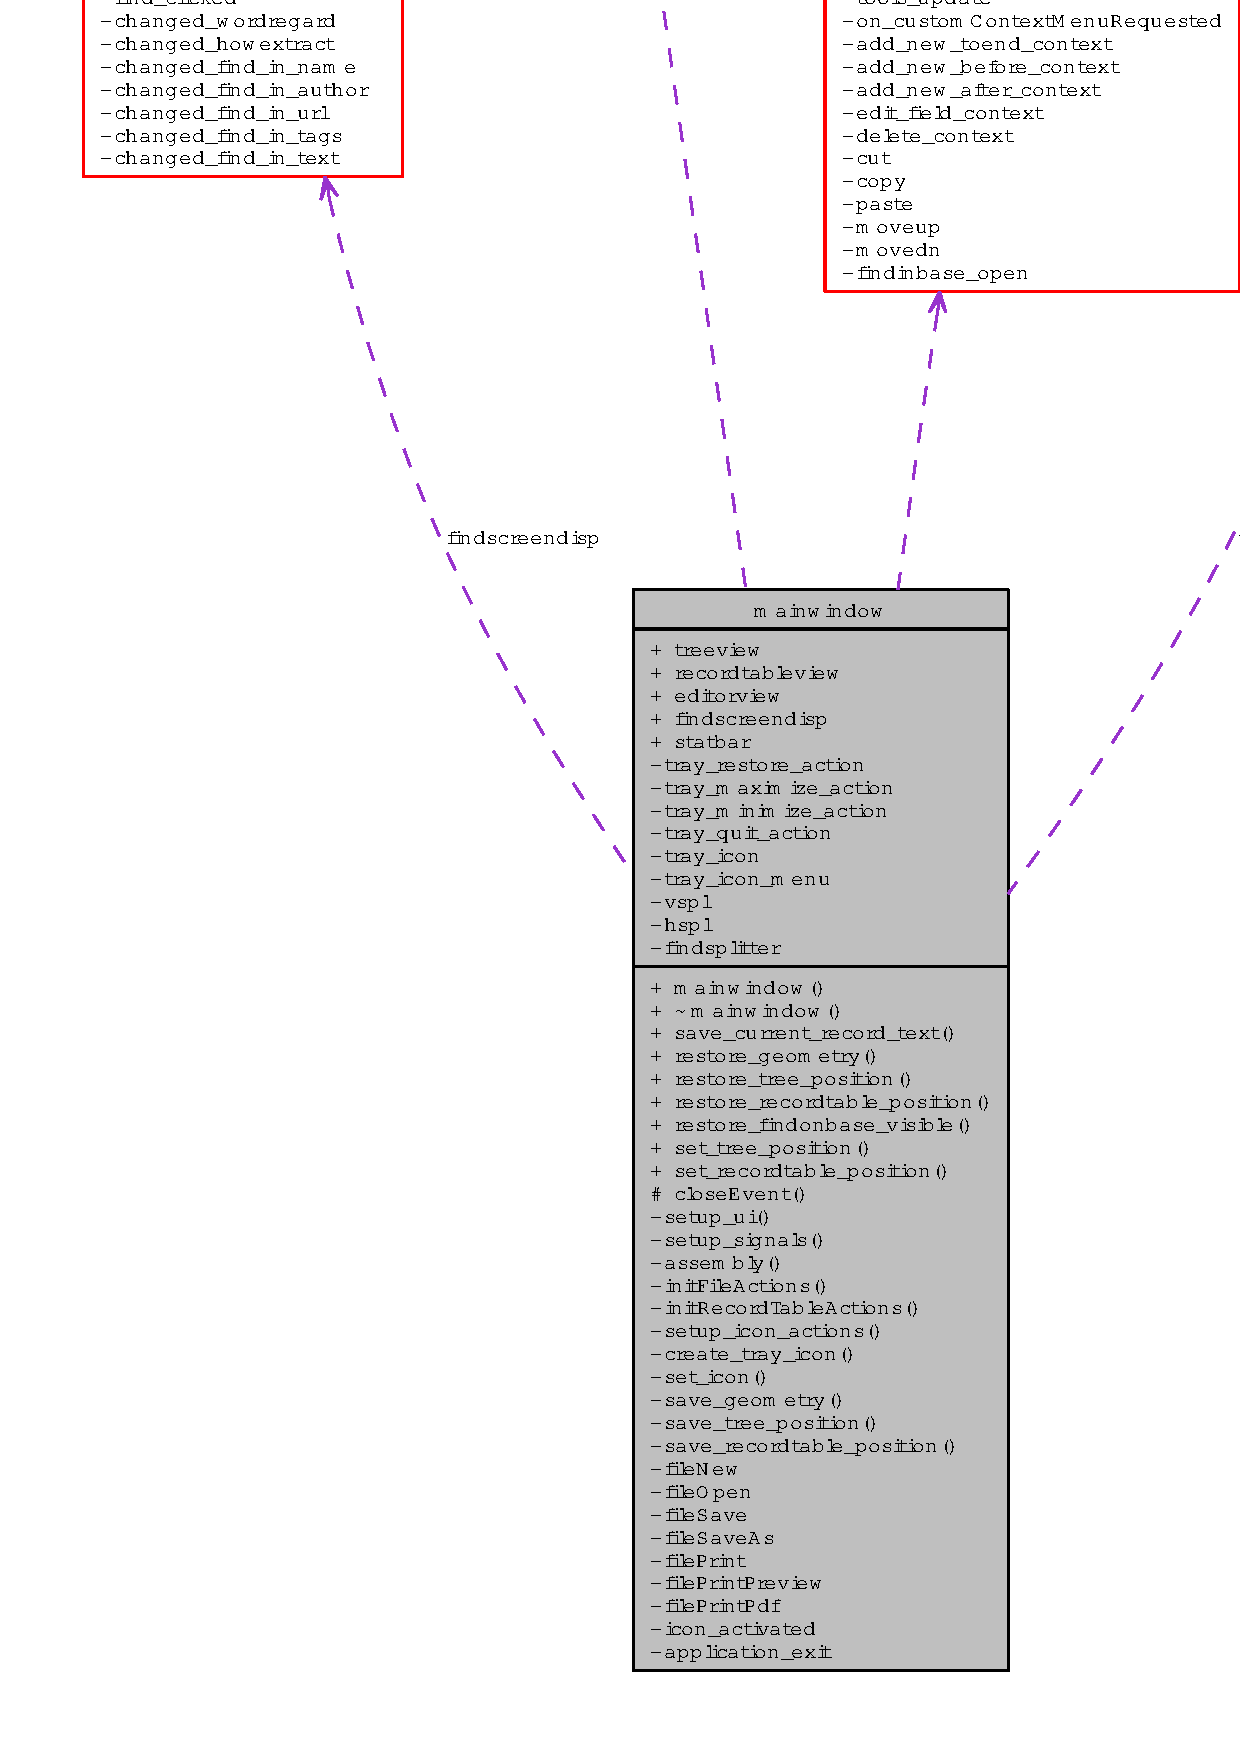
\includegraphics[width=407pt]{classmainwindow__coll__graph}
\end{center}
\end{figure}
\subsection*{Public Member Functions}
\begin{CompactItemize}
\item 
{\bf mainwindow} ()
\item 
{\bf $\sim$mainwindow} ()
\item 
void {\bf save\_\-current\_\-record\_\-text} (void)
\item 
void {\bf restore\_\-geometry} (void)
\item 
void {\bf restore\_\-tree\_\-position} (void)
\item 
void {\bf restore\_\-recordtable\_\-position} (void)
\item 
void {\bf restore\_\-findonbase\_\-visible} (void)
\item 
void {\bf set\_\-tree\_\-position} (QString\-List path)
\item 
void {\bf set\_\-recordtable\_\-position} (int n)
\end{CompactItemize}
\subsection*{Public Attributes}
\begin{CompactItemize}
\item 
{\bf treescreen} $\ast$ {\bf treeview}
\item 
{\bf recordtablescreen} $\ast$ {\bf recordtableview}
\item 
{\bf metaeditor} $\ast$ {\bf editorview}
\item 
{\bf findscreen} $\ast$ {\bf findscreendisp}
\item 
QStatus\-Bar $\ast$ {\bf statbar}
\end{CompactItemize}
\subsection*{Protected Member Functions}
\begin{CompactItemize}
\item 
void {\bf close\-Event} (QClose\-Event $\ast$event)
\end{CompactItemize}
\subsection*{Private Slots}
\begin{CompactItemize}
\item 
void {\bf file\-New} (void)
\item 
void {\bf file\-Open} (void)
\item 
bool {\bf file\-Save} (void)
\item 
bool {\bf file\-Save\-As} (void)
\item 
void {\bf file\-Print} (void)
\item 
void {\bf file\-Print\-Preview} (void)
\item 
void {\bf file\-Print\-Pdf} (void)
\item 
void {\bf icon\_\-activated} (QSystem\-Tray\-Icon::Activation\-Reason reason)
\item 
void {\bf application\_\-exit} (void)
\end{CompactItemize}
\subsection*{Private Member Functions}
\begin{CompactItemize}
\item 
void {\bf setup\_\-ui} (void)
\item 
void {\bf setup\_\-signals} (void)
\item 
void {\bf assembly} (void)
\item 
void {\bf init\-File\-Actions} (void)
\item 
void {\bf init\-Record\-Table\-Actions} (void)
\item 
void {\bf setup\_\-icon\_\-actions} (void)
\item 
void {\bf create\_\-tray\_\-icon} (void)
\item 
void {\bf set\_\-icon} (void)
\item 
void {\bf save\_\-geometry} (void)
\item 
void {\bf save\_\-tree\_\-position} (void)
\item 
void {\bf save\_\-recordtable\_\-position} (void)
\end{CompactItemize}
\subsection*{Private Attributes}
\begin{CompactItemize}
\item 
QAction $\ast$ {\bf tray\_\-restore\_\-action}
\item 
QAction $\ast$ {\bf tray\_\-maximize\_\-action}
\item 
QAction $\ast$ {\bf tray\_\-minimize\_\-action}
\item 
QAction $\ast$ {\bf tray\_\-quit\_\-action}
\item 
QSystem\-Tray\-Icon $\ast$ {\bf tray\_\-icon}
\item 
QMenu $\ast$ {\bf tray\_\-icon\_\-menu}
\item 
QSplitter $\ast$ {\bf vspl}
\item 
QSplitter $\ast$ {\bf hspl}
\item 
QSplitter $\ast$ {\bf findsplitter}
\end{CompactItemize}


\subsection{Detailed Description}




Definition at line 71 of file mainwindow.h.

\subsection{Constructor \& Destructor Documentation}
\index{mainwindow@{mainwindow}!mainwindow@{mainwindow}}
\index{mainwindow@{mainwindow}!mainwindow@{mainwindow}}
\subsubsection{\setlength{\rightskip}{0pt plus 5cm}mainwindow::mainwindow ()}\label{classmainwindow_b3362dc64d962bffa152d883b3de8a29}




Definition at line 11 of file mainwindow.cpp.

References assembly(), create\_\-tray\_\-icon(), init\-File\-Actions(), set\_\-icon(), setup\_\-icon\_\-actions(), setup\_\-signals(), setup\_\-ui(), and tray\_\-icon.

Here is the call graph for this function:\begin{figure}[H]
\begin{center}
\leavevmode
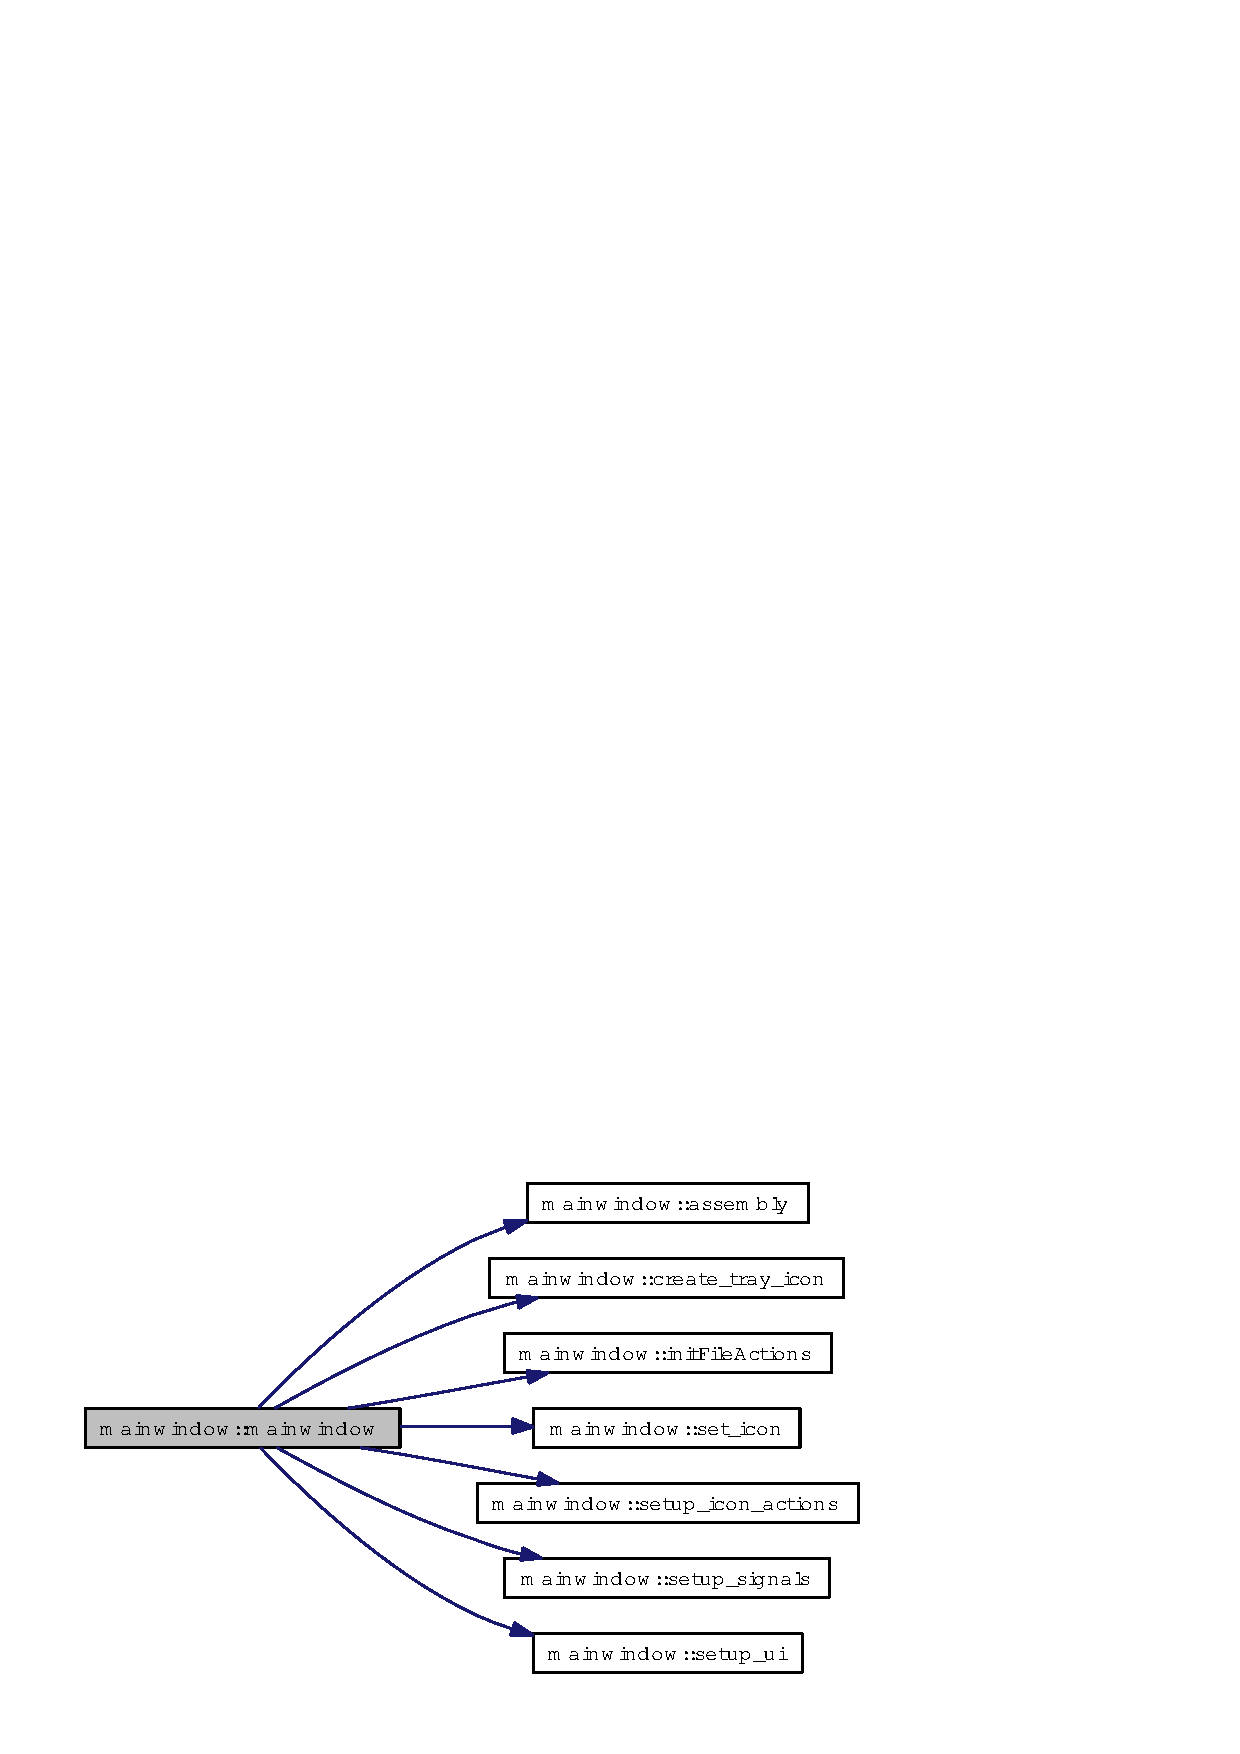
\includegraphics[width=208pt]{classmainwindow_b3362dc64d962bffa152d883b3de8a29_cgraph}
\end{center}
\end{figure}
\index{mainwindow@{mainwindow}!~mainwindow@{$\sim$mainwindow}}
\index{~mainwindow@{$\sim$mainwindow}!mainwindow@{mainwindow}}
\subsubsection{\setlength{\rightskip}{0pt plus 5cm}mainwindow::$\sim$mainwindow ()}\label{classmainwindow_5443e012964c892ef6015e7cebf62a67}




Definition at line 27 of file mainwindow.cpp.

References editorview, recordtableview, save\_\-current\_\-record\_\-text(), save\_\-geometry(), save\_\-recordtable\_\-position(), save\_\-tree\_\-position(), and treeview.

Here is the call graph for this function:\begin{figure}[H]
\begin{center}
\leavevmode
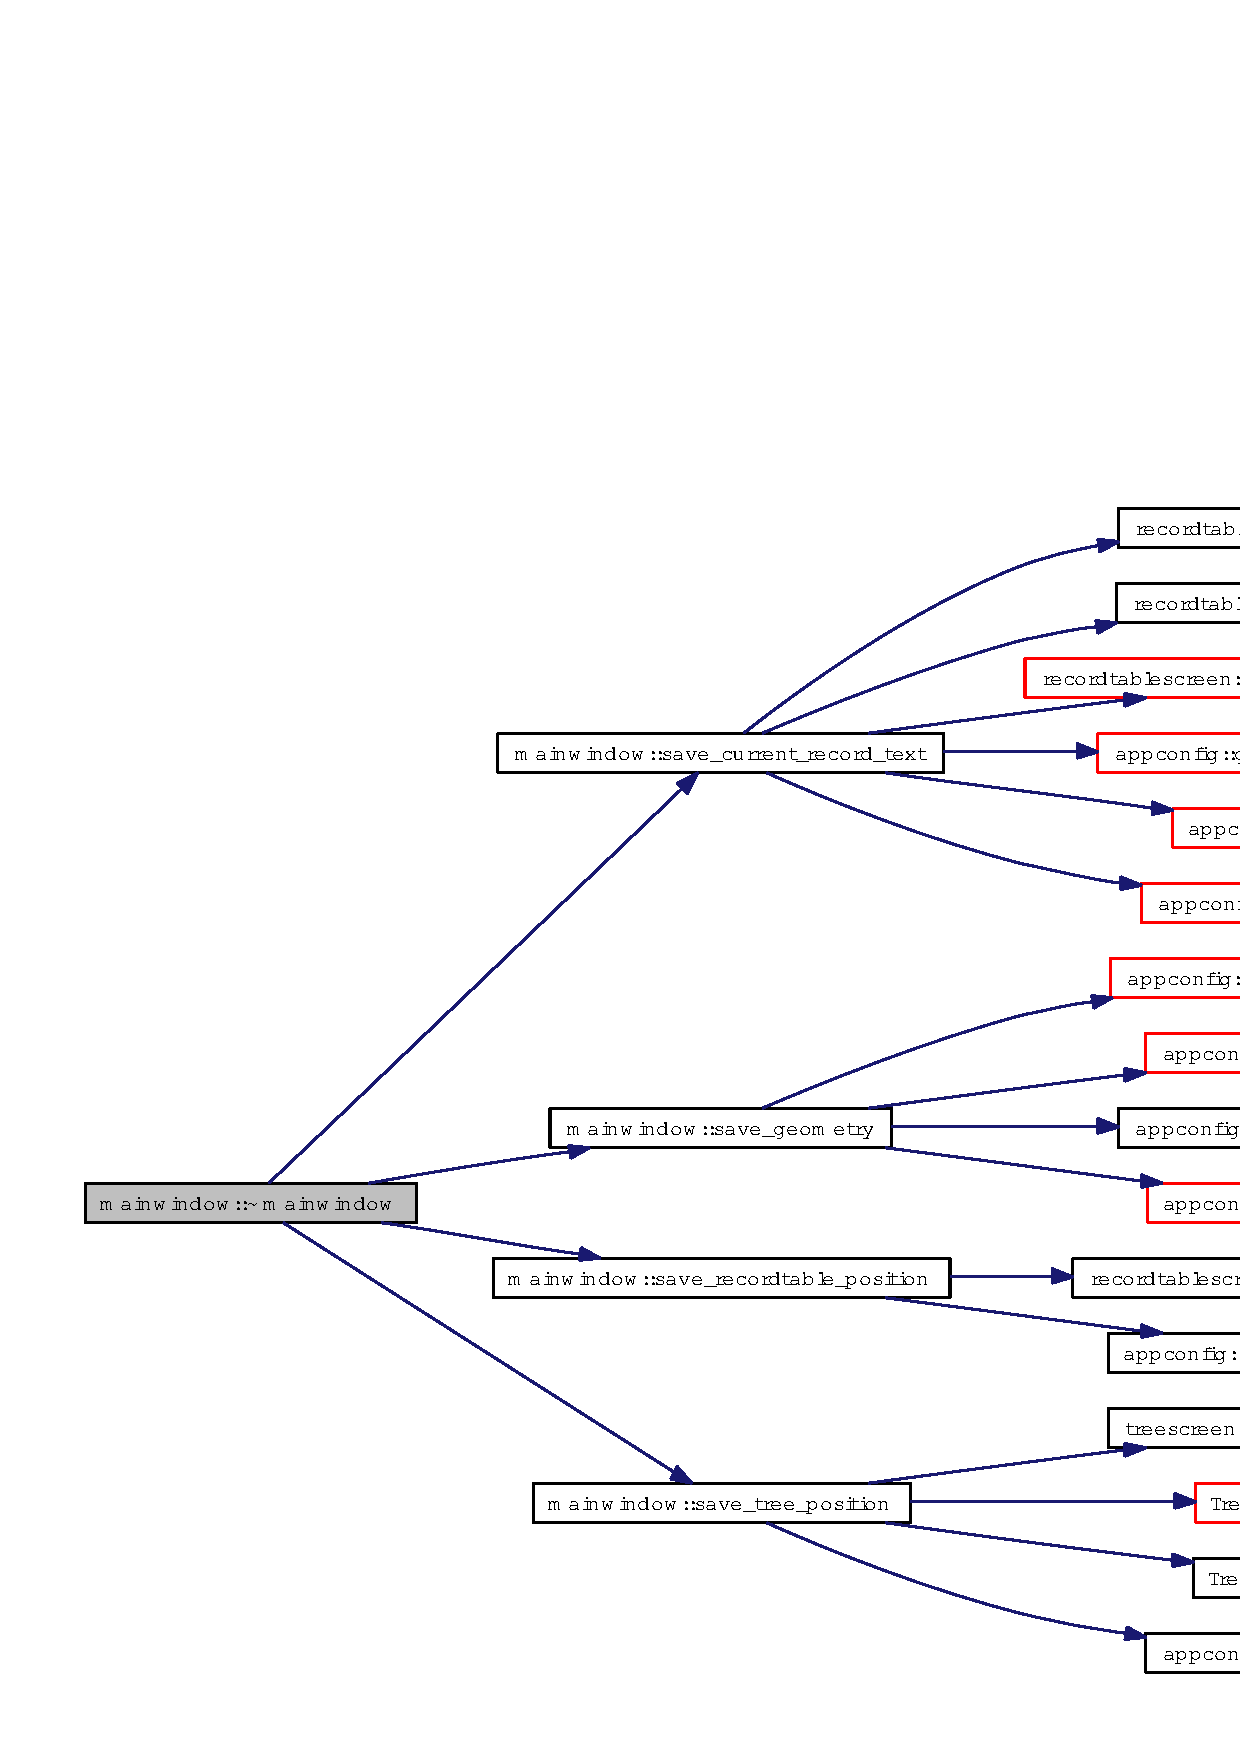
\includegraphics[width=386pt]{classmainwindow_5443e012964c892ef6015e7cebf62a67_cgraph}
\end{center}
\end{figure}


\subsection{Member Function Documentation}
\index{mainwindow@{mainwindow}!save_current_record_text@{save\_\-current\_\-record\_\-text}}
\index{save_current_record_text@{save\_\-current\_\-record\_\-text}!mainwindow@{mainwindow}}
\subsubsection{\setlength{\rightskip}{0pt plus 5cm}void mainwindow::save\_\-current\_\-record\_\-text (void)}\label{classmainwindow_5584aaad939eac61d3e5e9e09e666016}




Definition at line 415 of file mainwindow.cpp.

References editorview, recordtablescreen::get\_\-currentdir(), recordtablescreen::get\_\-currentfile(), recordtablescreen::get\_\-fullfilename\_\-of\_\-currentitem(), appconfig::get\_\-lastprefixnum\_\-as\_\-line(), appconfig::get\_\-trashdir(), appconfig::inc\_\-lastprefixnum(), mytetraconfig, recordtableview, and editor::textarea.

Referenced by $\sim$mainwindow().

Here is the call graph for this function:\begin{figure}[H]
\begin{center}
\leavevmode
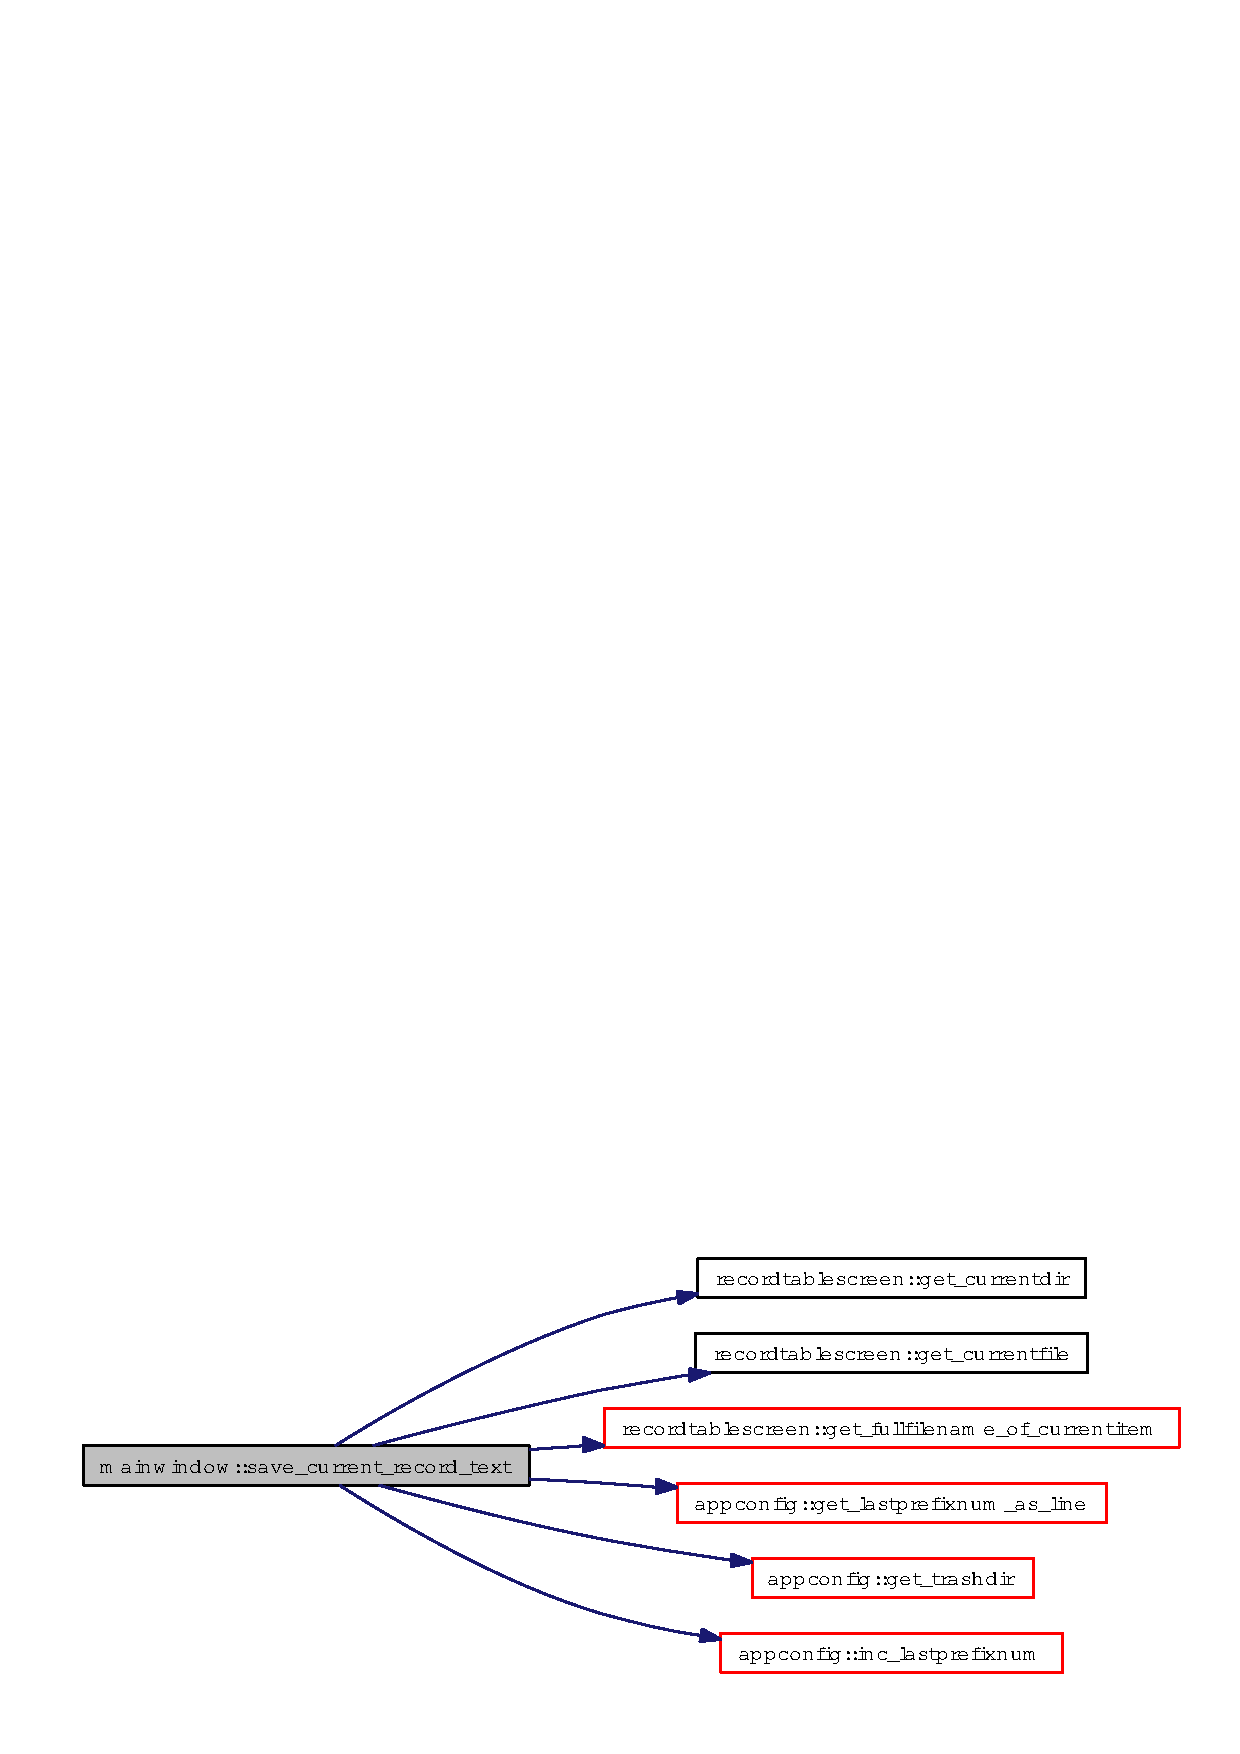
\includegraphics[width=285pt]{classmainwindow_5584aaad939eac61d3e5e9e09e666016_cgraph}
\end{center}
\end{figure}


Here is the caller graph for this function:\begin{figure}[H]
\begin{center}
\leavevmode
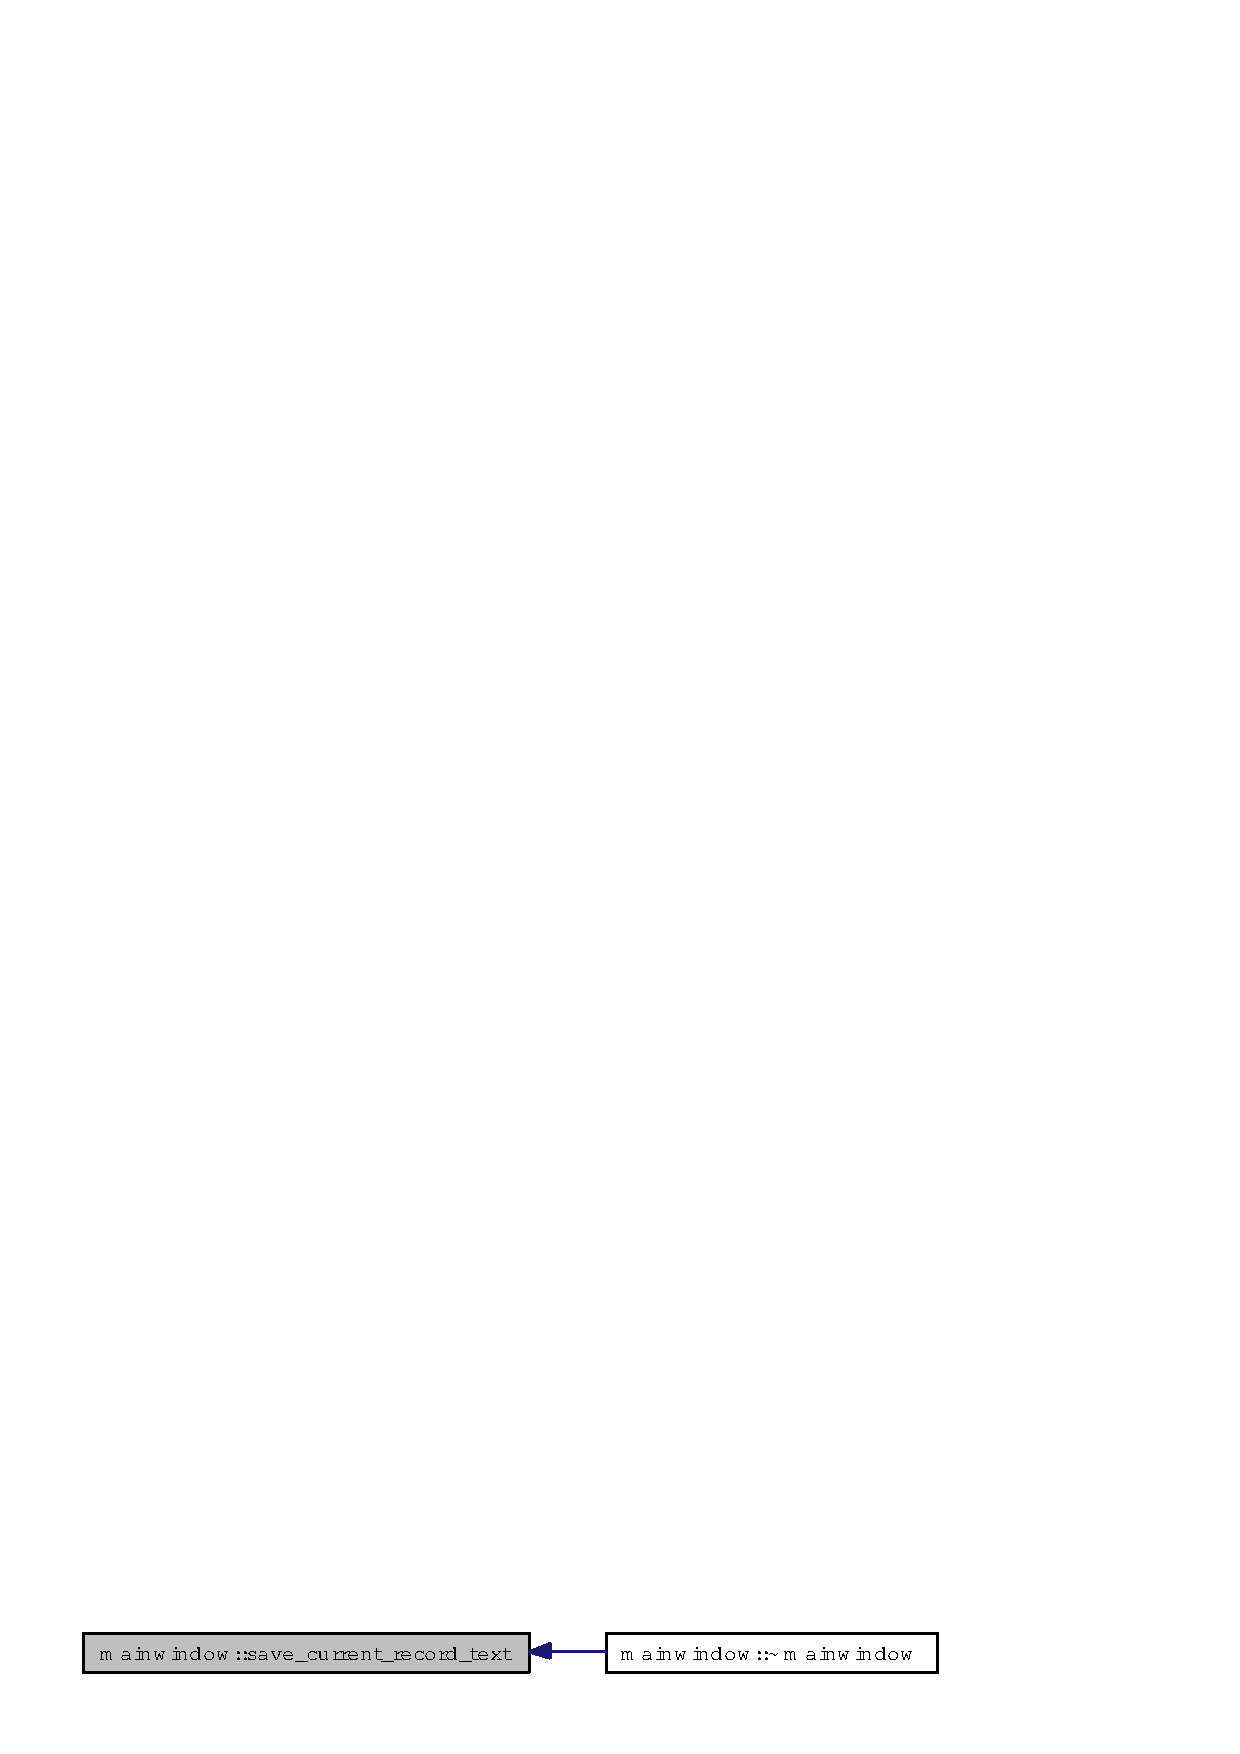
\includegraphics[width=227pt]{classmainwindow_5584aaad939eac61d3e5e9e09e666016_icgraph}
\end{center}
\end{figure}
\index{mainwindow@{mainwindow}!restore_geometry@{restore\_\-geometry}}
\index{restore_geometry@{restore\_\-geometry}!mainwindow@{mainwindow}}
\subsubsection{\setlength{\rightskip}{0pt plus 5cm}void mainwindow::restore\_\-geometry (void)}\label{classmainwindow_79369c37683c95e6e95928571e047100}




Definition at line 96 of file mainwindow.cpp.

References findsplitter, appconfig::get\_\-findsplitter\_\-size\_\-list(), appconfig::get\_\-hspl\_\-size\_\-list(), appconfig::get\_\-mainwingeometry(), appconfig::get\_\-vspl\_\-size\_\-list(), hspl, mytetraconfig, and vspl.

Referenced by main().

Here is the call graph for this function:\begin{figure}[H]
\begin{center}
\leavevmode
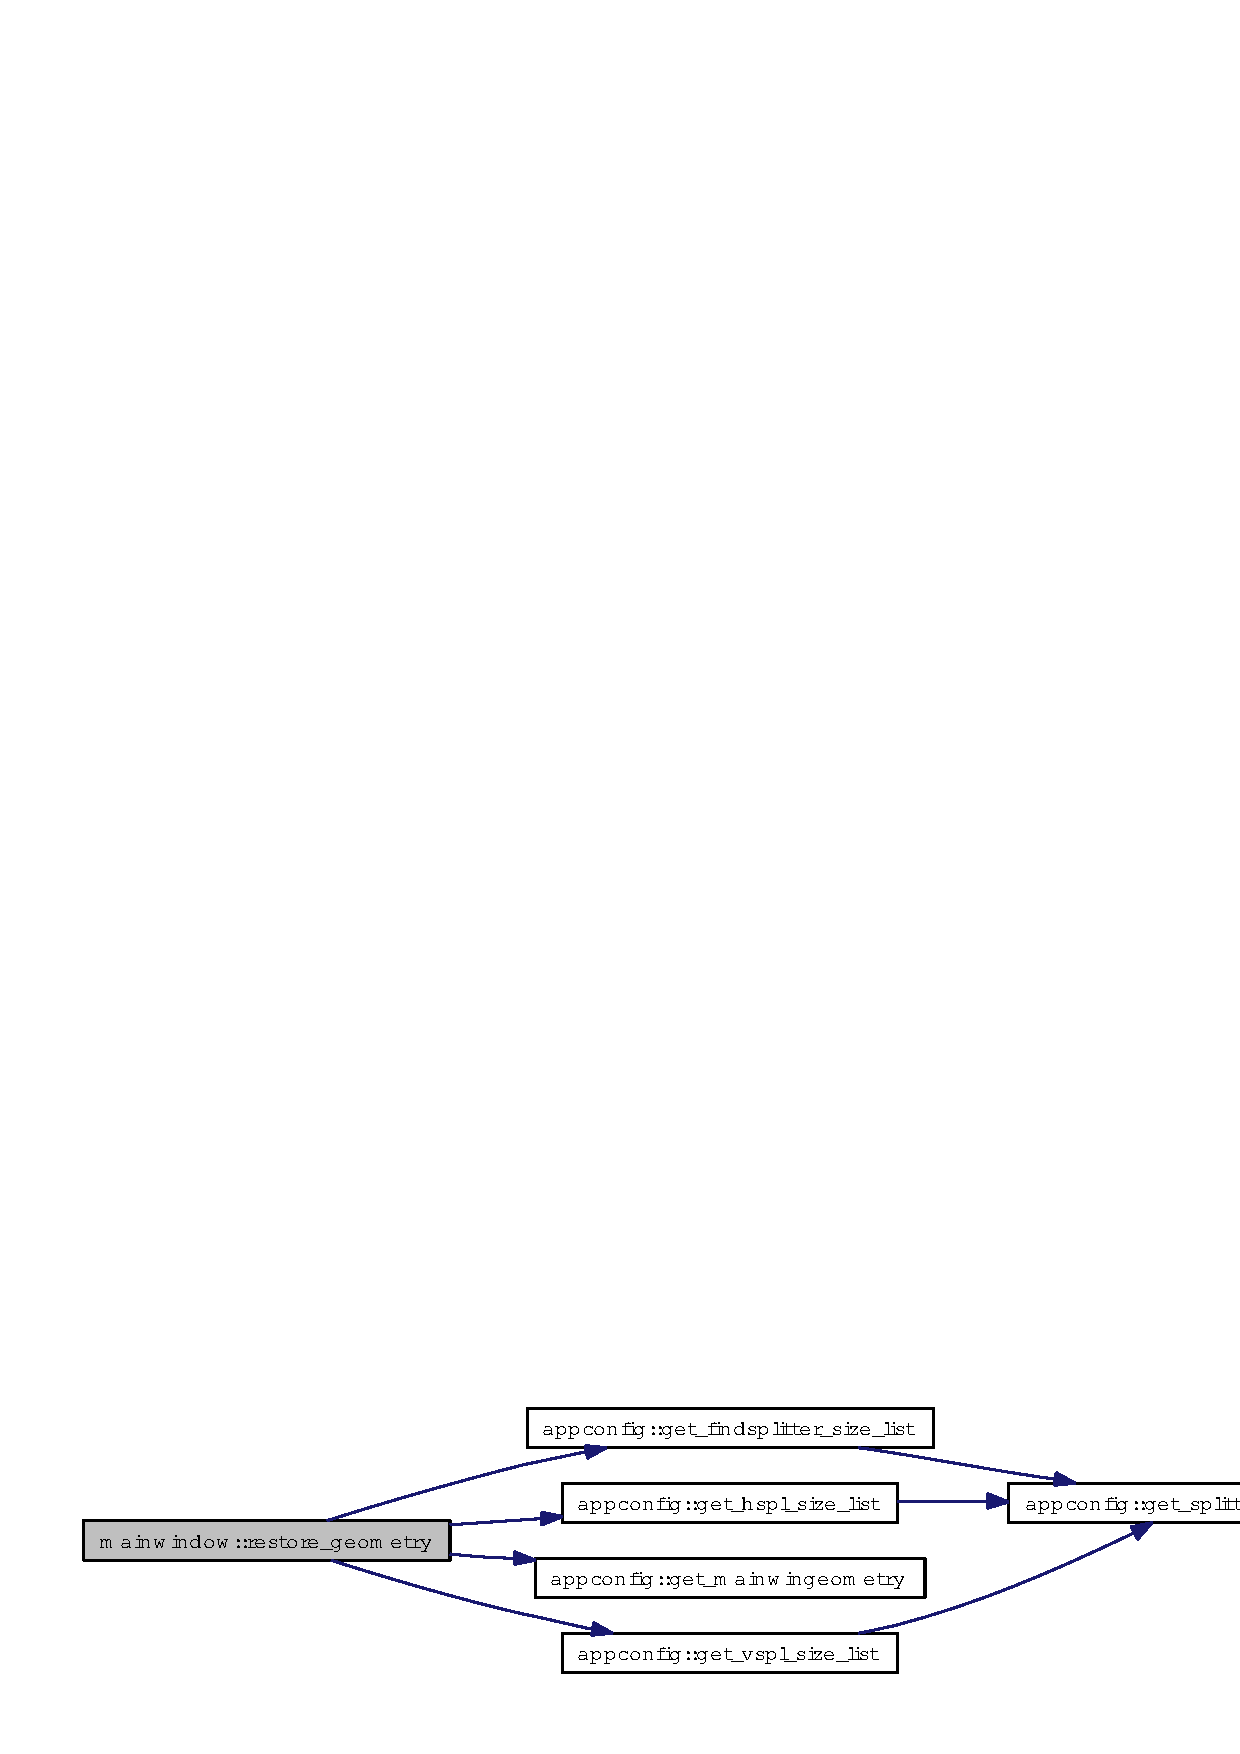
\includegraphics[width=332pt]{classmainwindow_79369c37683c95e6e95928571e047100_cgraph}
\end{center}
\end{figure}


Here is the caller graph for this function:\begin{figure}[H]
\begin{center}
\leavevmode
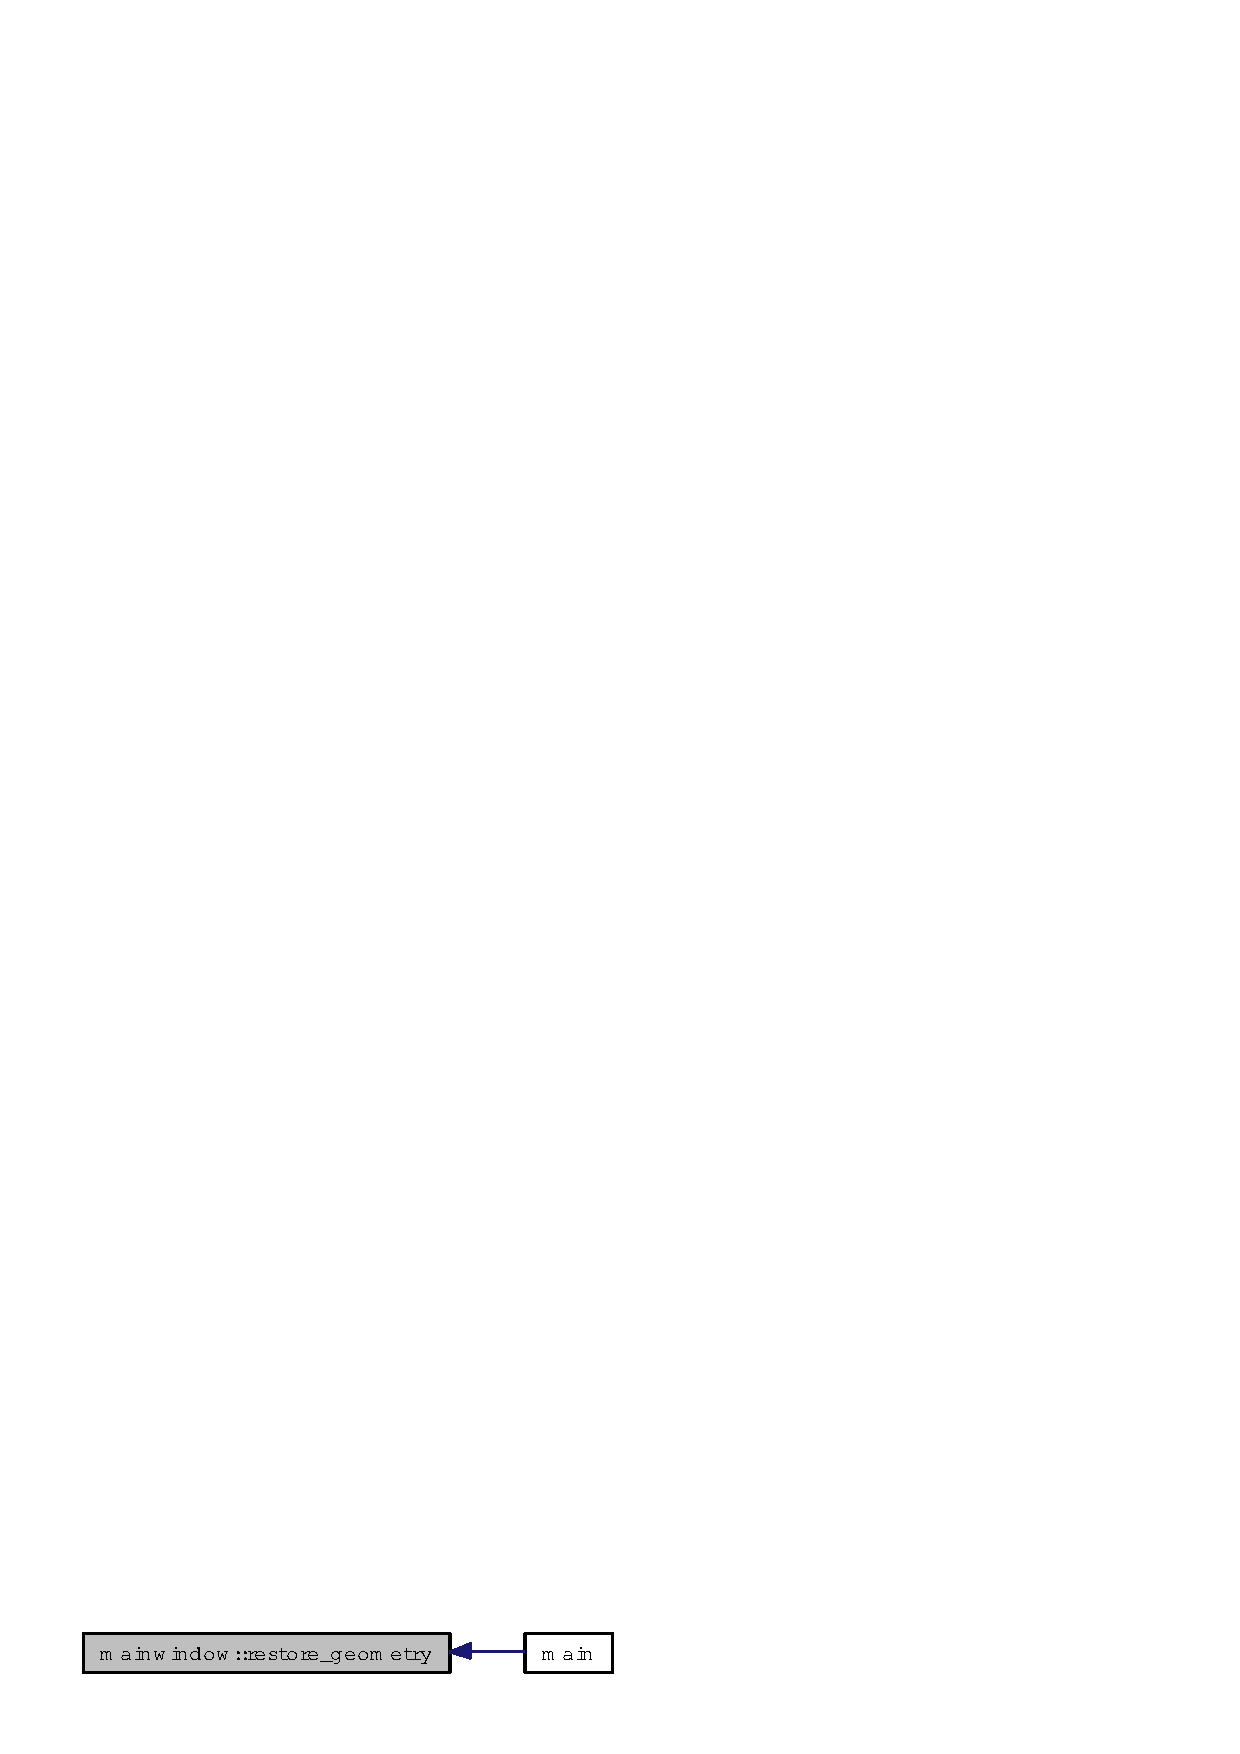
\includegraphics[width=149pt]{classmainwindow_79369c37683c95e6e95928571e047100_icgraph}
\end{center}
\end{figure}
\index{mainwindow@{mainwindow}!restore_tree_position@{restore\_\-tree\_\-position}}
\index{restore_tree_position@{restore\_\-tree\_\-position}!mainwindow@{mainwindow}}
\subsubsection{\setlength{\rightskip}{0pt plus 5cm}void mainwindow::restore\_\-tree\_\-position (void)}\label{classmainwindow_8337021add562a78f8f702173d541455}




Definition at line 124 of file mainwindow.cpp.

References appconfig::get\_\-tree\_\-position(), mytetraconfig, and set\_\-tree\_\-position().

Referenced by main().

Here is the call graph for this function:\begin{figure}[H]
\begin{center}
\leavevmode
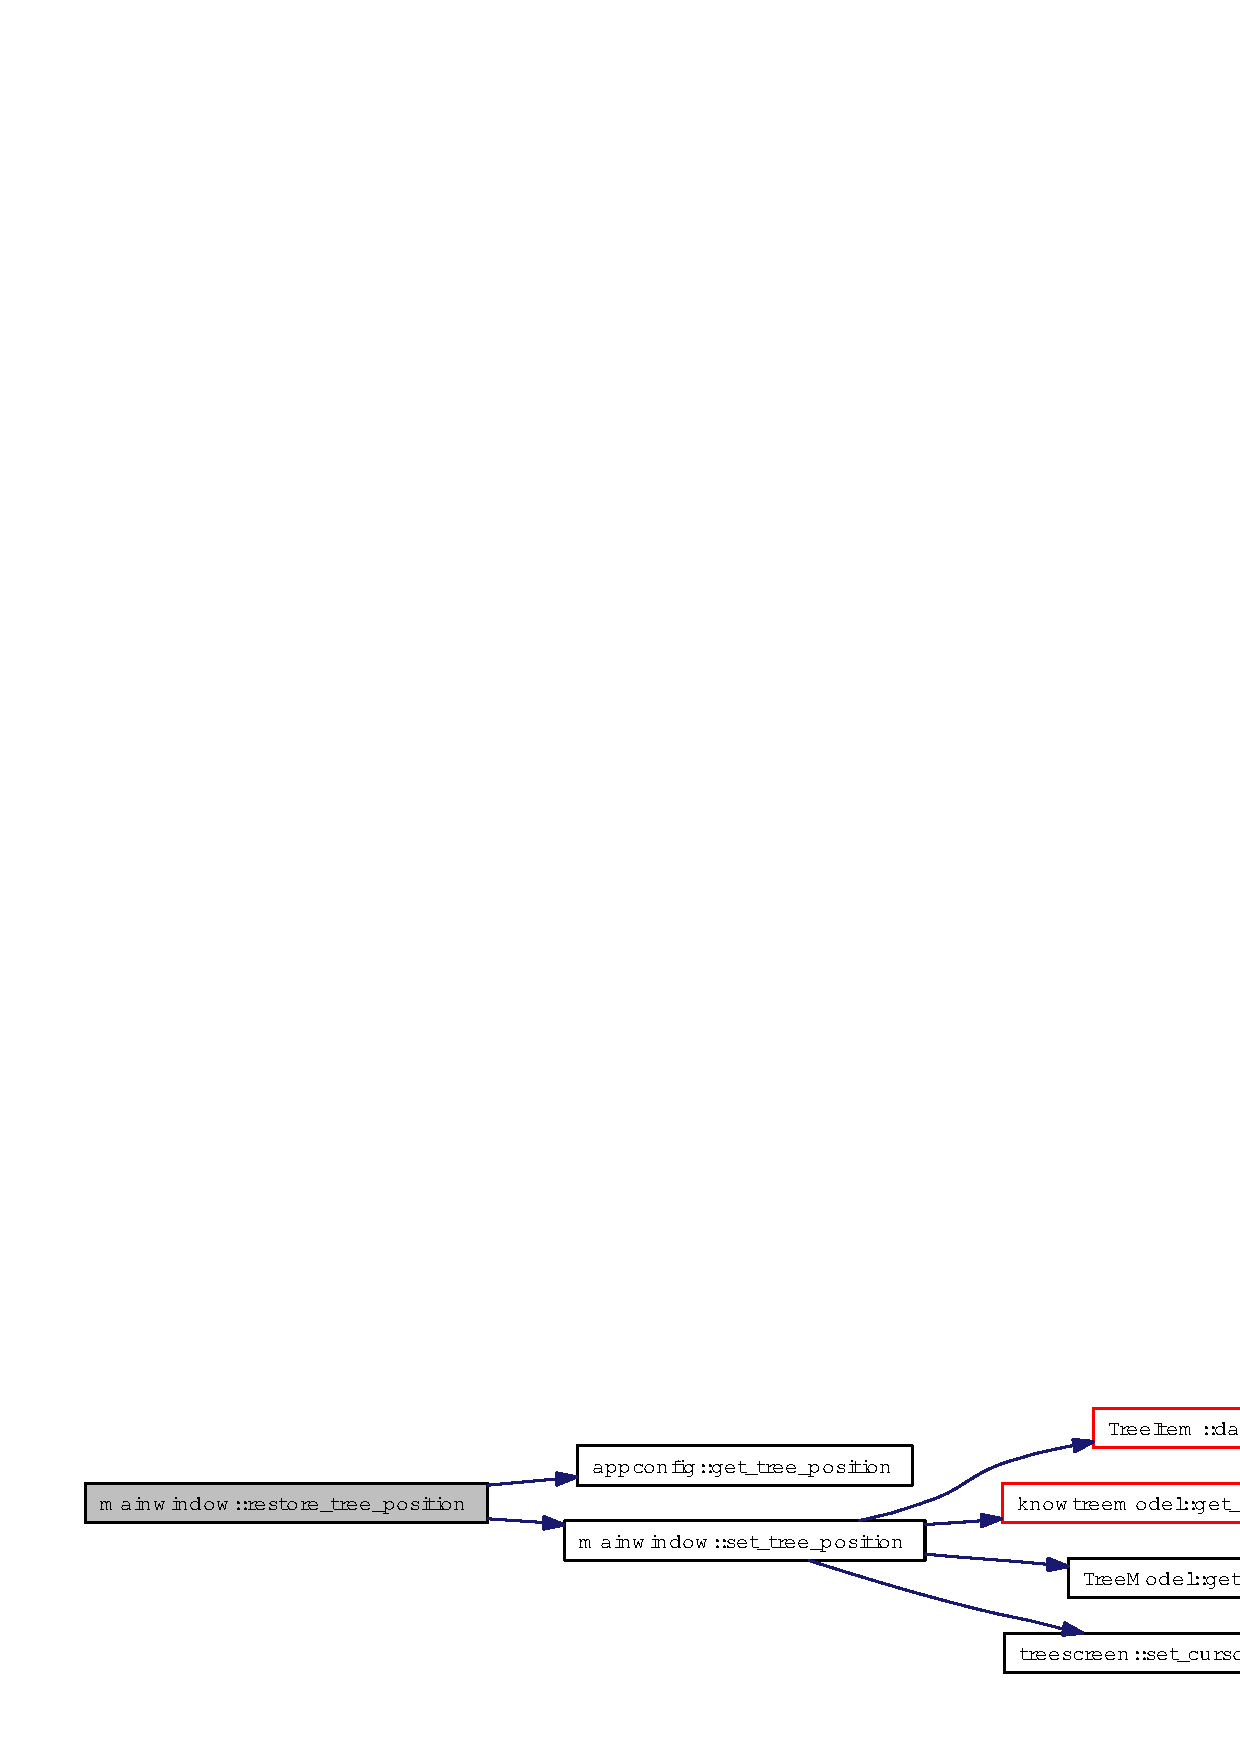
\includegraphics[width=332pt]{classmainwindow_8337021add562a78f8f702173d541455_cgraph}
\end{center}
\end{figure}


Here is the caller graph for this function:\begin{figure}[H]
\begin{center}
\leavevmode
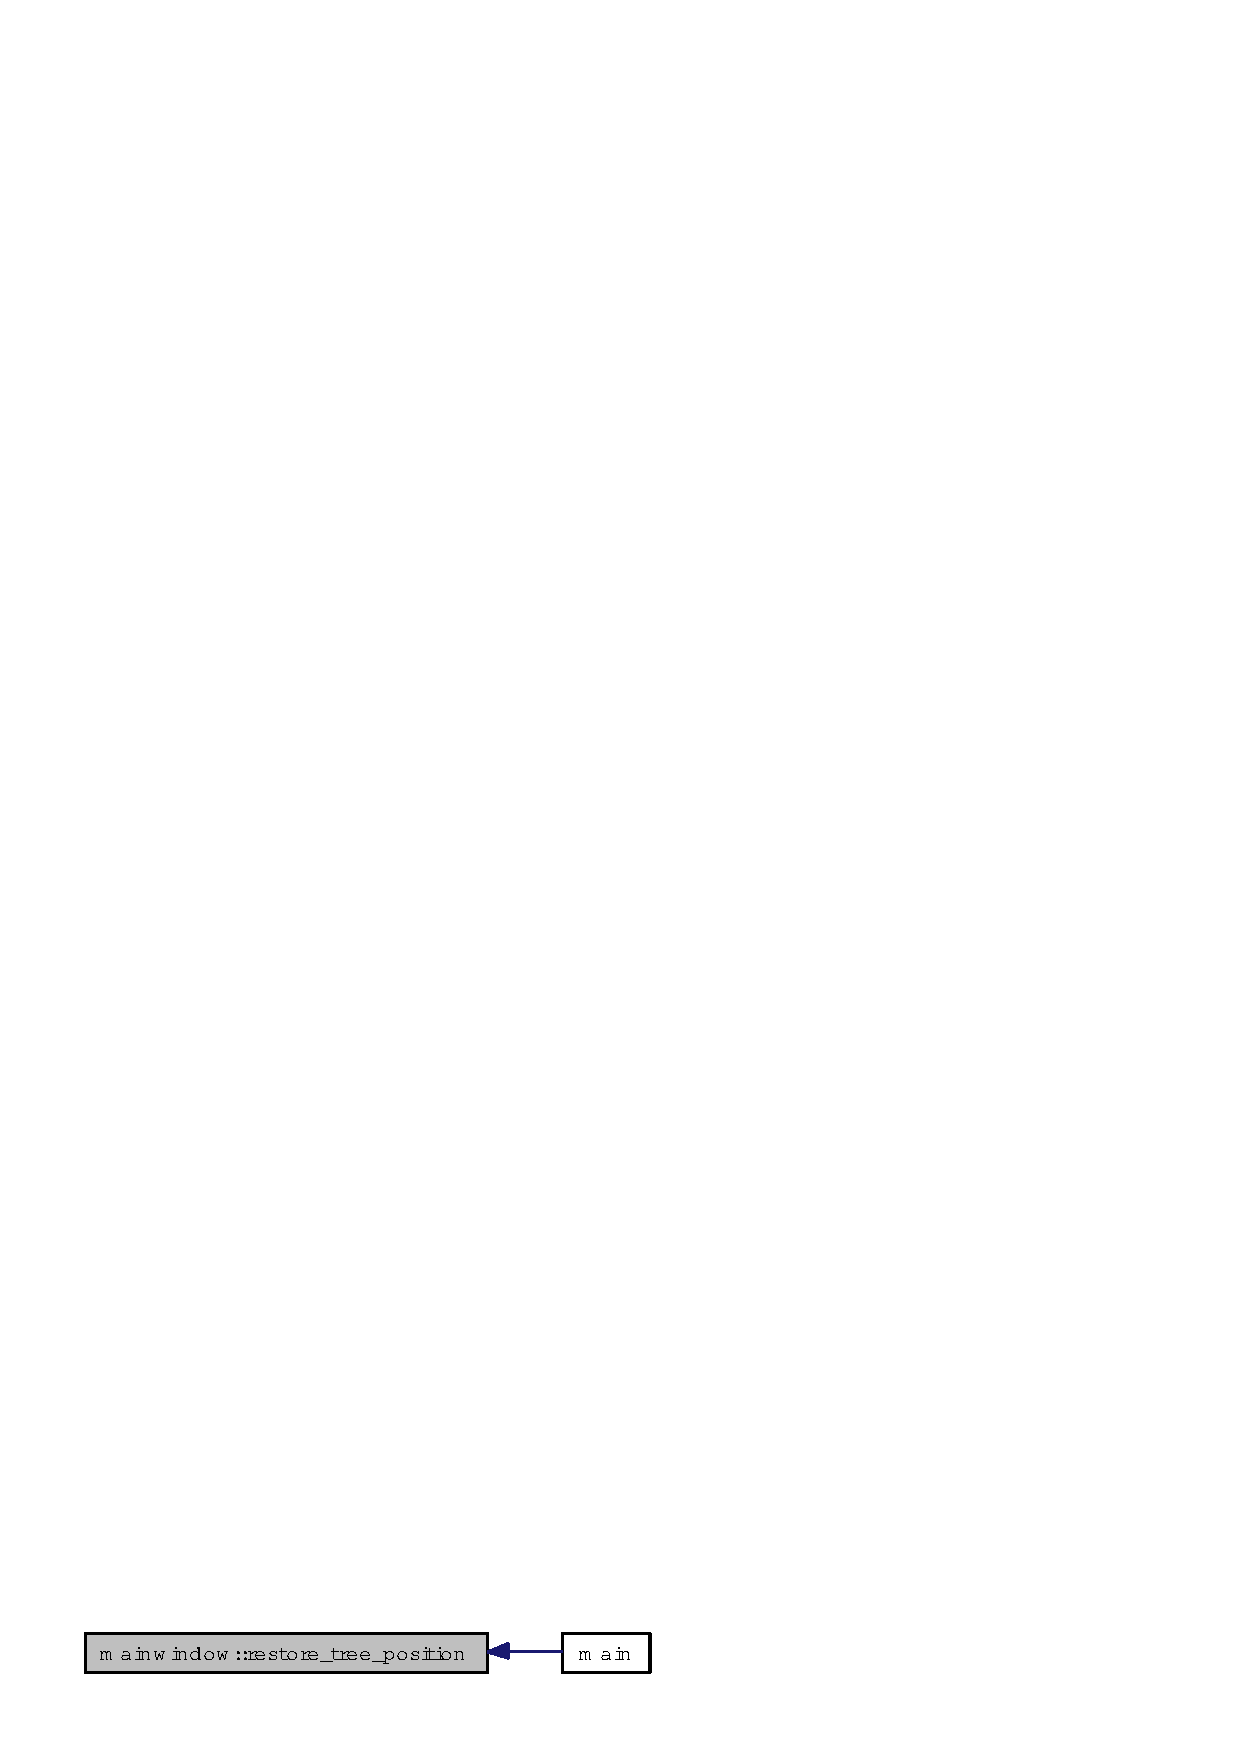
\includegraphics[width=158pt]{classmainwindow_8337021add562a78f8f702173d541455_icgraph}
\end{center}
\end{figure}
\index{mainwindow@{mainwindow}!restore_recordtable_position@{restore\_\-recordtable\_\-position}}
\index{restore_recordtable_position@{restore\_\-recordtable\_\-position}!mainwindow@{mainwindow}}
\subsubsection{\setlength{\rightskip}{0pt plus 5cm}void mainwindow::restore\_\-recordtable\_\-position (void)}\label{classmainwindow_555e2cff5de029fedcf796372d57386a}




Definition at line 161 of file mainwindow.cpp.

References appconfig::get\_\-recordtable\_\-position(), mytetraconfig, and set\_\-recordtable\_\-position().

Referenced by main().

Here is the call graph for this function:\begin{figure}[H]
\begin{center}
\leavevmode
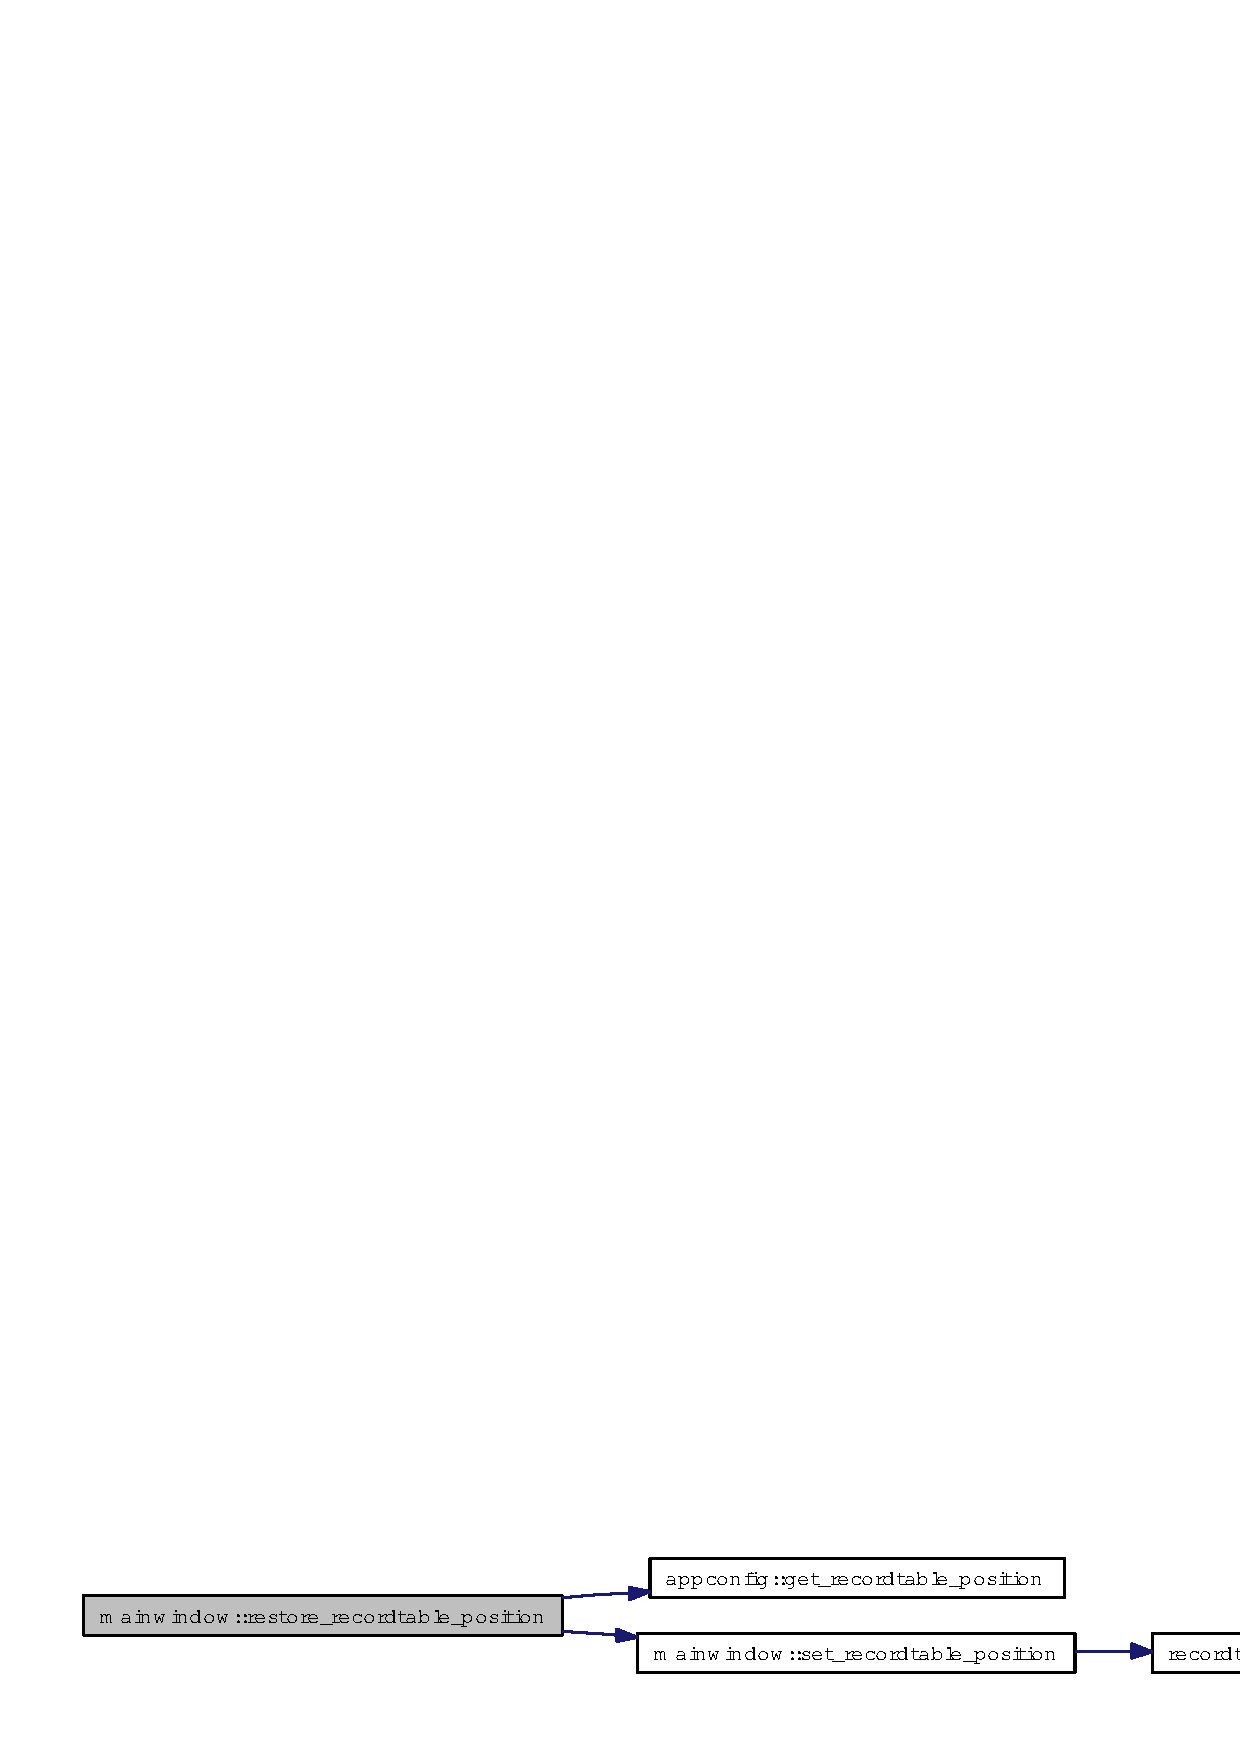
\includegraphics[width=388pt]{classmainwindow_555e2cff5de029fedcf796372d57386a_cgraph}
\end{center}
\end{figure}


Here is the caller graph for this function:\begin{figure}[H]
\begin{center}
\leavevmode
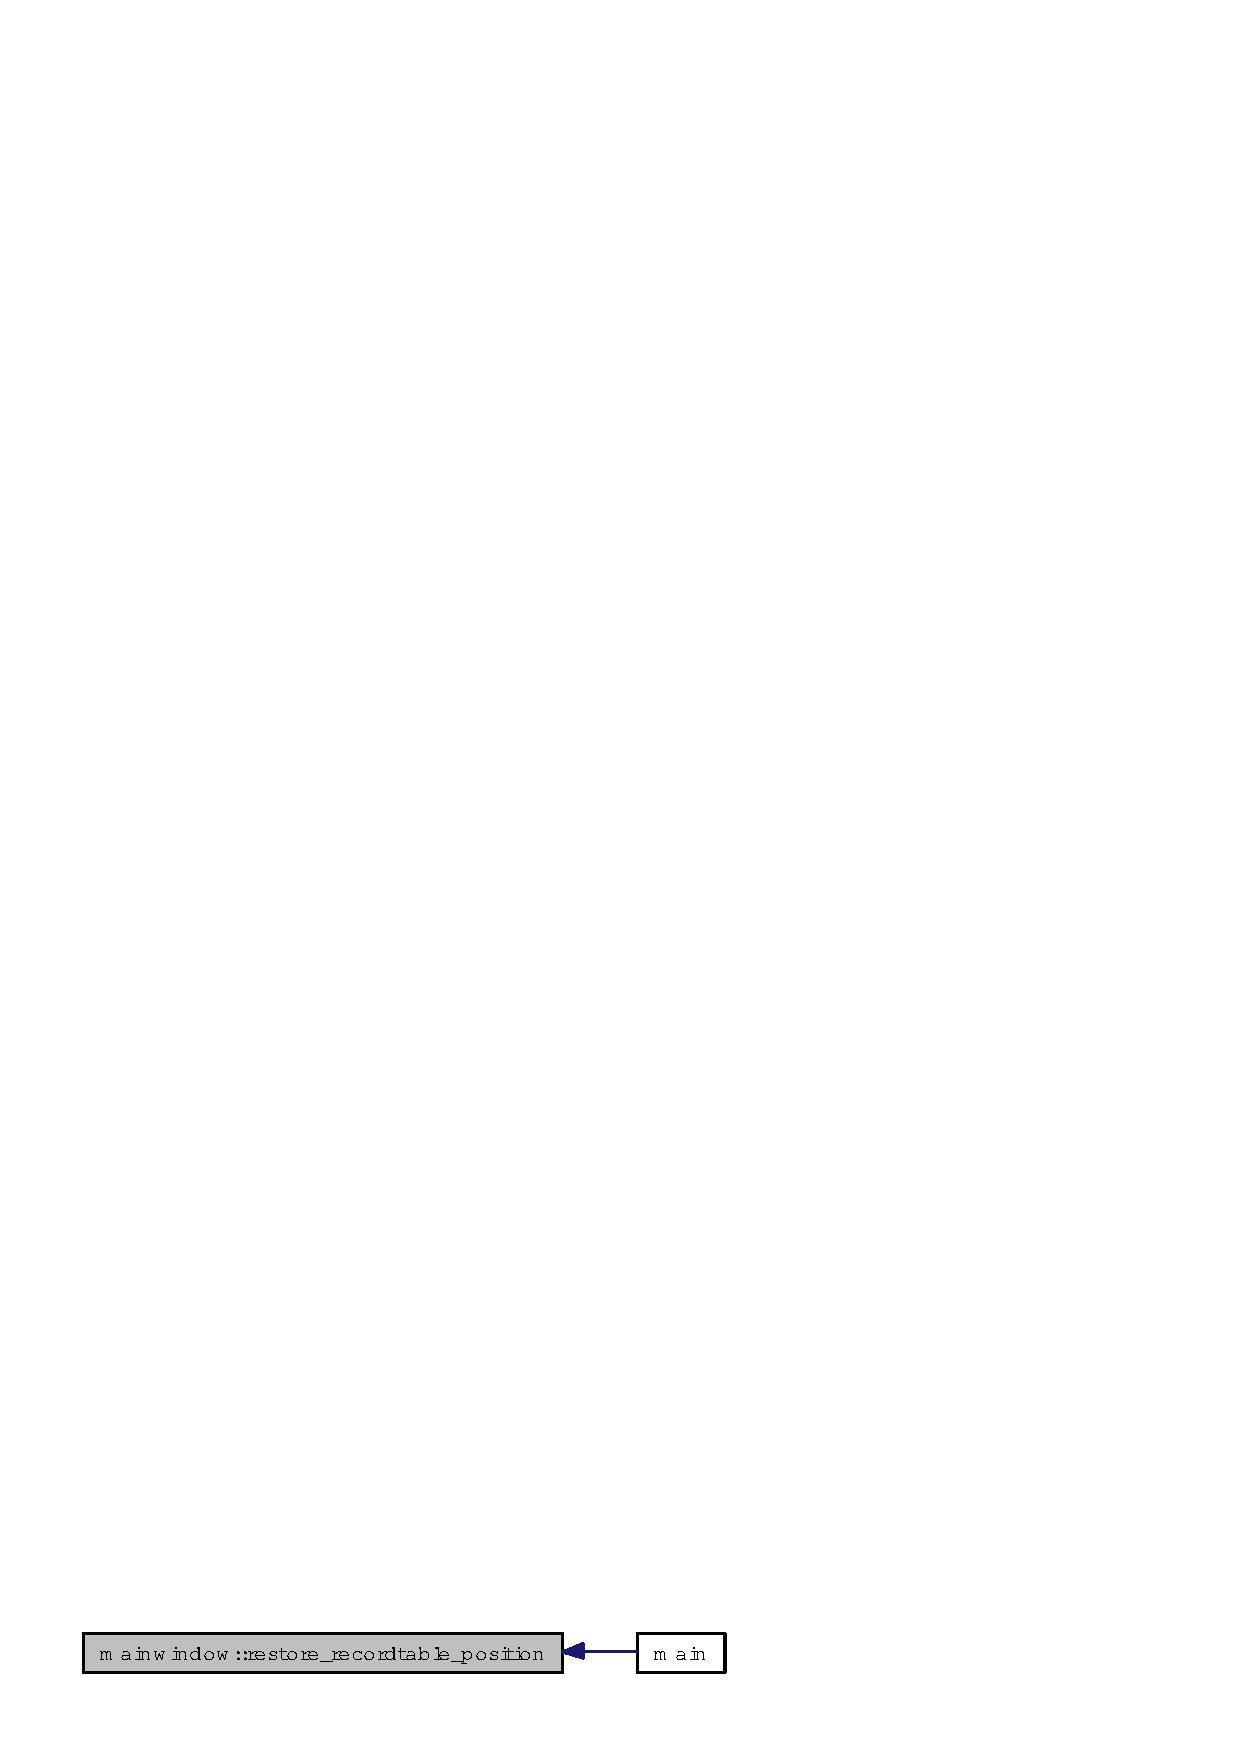
\includegraphics[width=176pt]{classmainwindow_555e2cff5de029fedcf796372d57386a_icgraph}
\end{center}
\end{figure}
\index{mainwindow@{mainwindow}!restore_findonbase_visible@{restore\_\-findonbase\_\-visible}}
\index{restore_findonbase_visible@{restore\_\-findonbase\_\-visible}!mainwindow@{mainwindow}}
\subsubsection{\setlength{\rightskip}{0pt plus 5cm}void mainwindow::restore\_\-findonbase\_\-visible (void)}\label{classmainwindow_676fda5aa4ca3b8d2d57c4521d69f00b}




Definition at line 183 of file mainwindow.cpp.

References appconfig::get\_\-findscreen\_\-show(), and mytetraconfig.

Referenced by main().

Here is the call graph for this function:\begin{figure}[H]
\begin{center}
\leavevmode
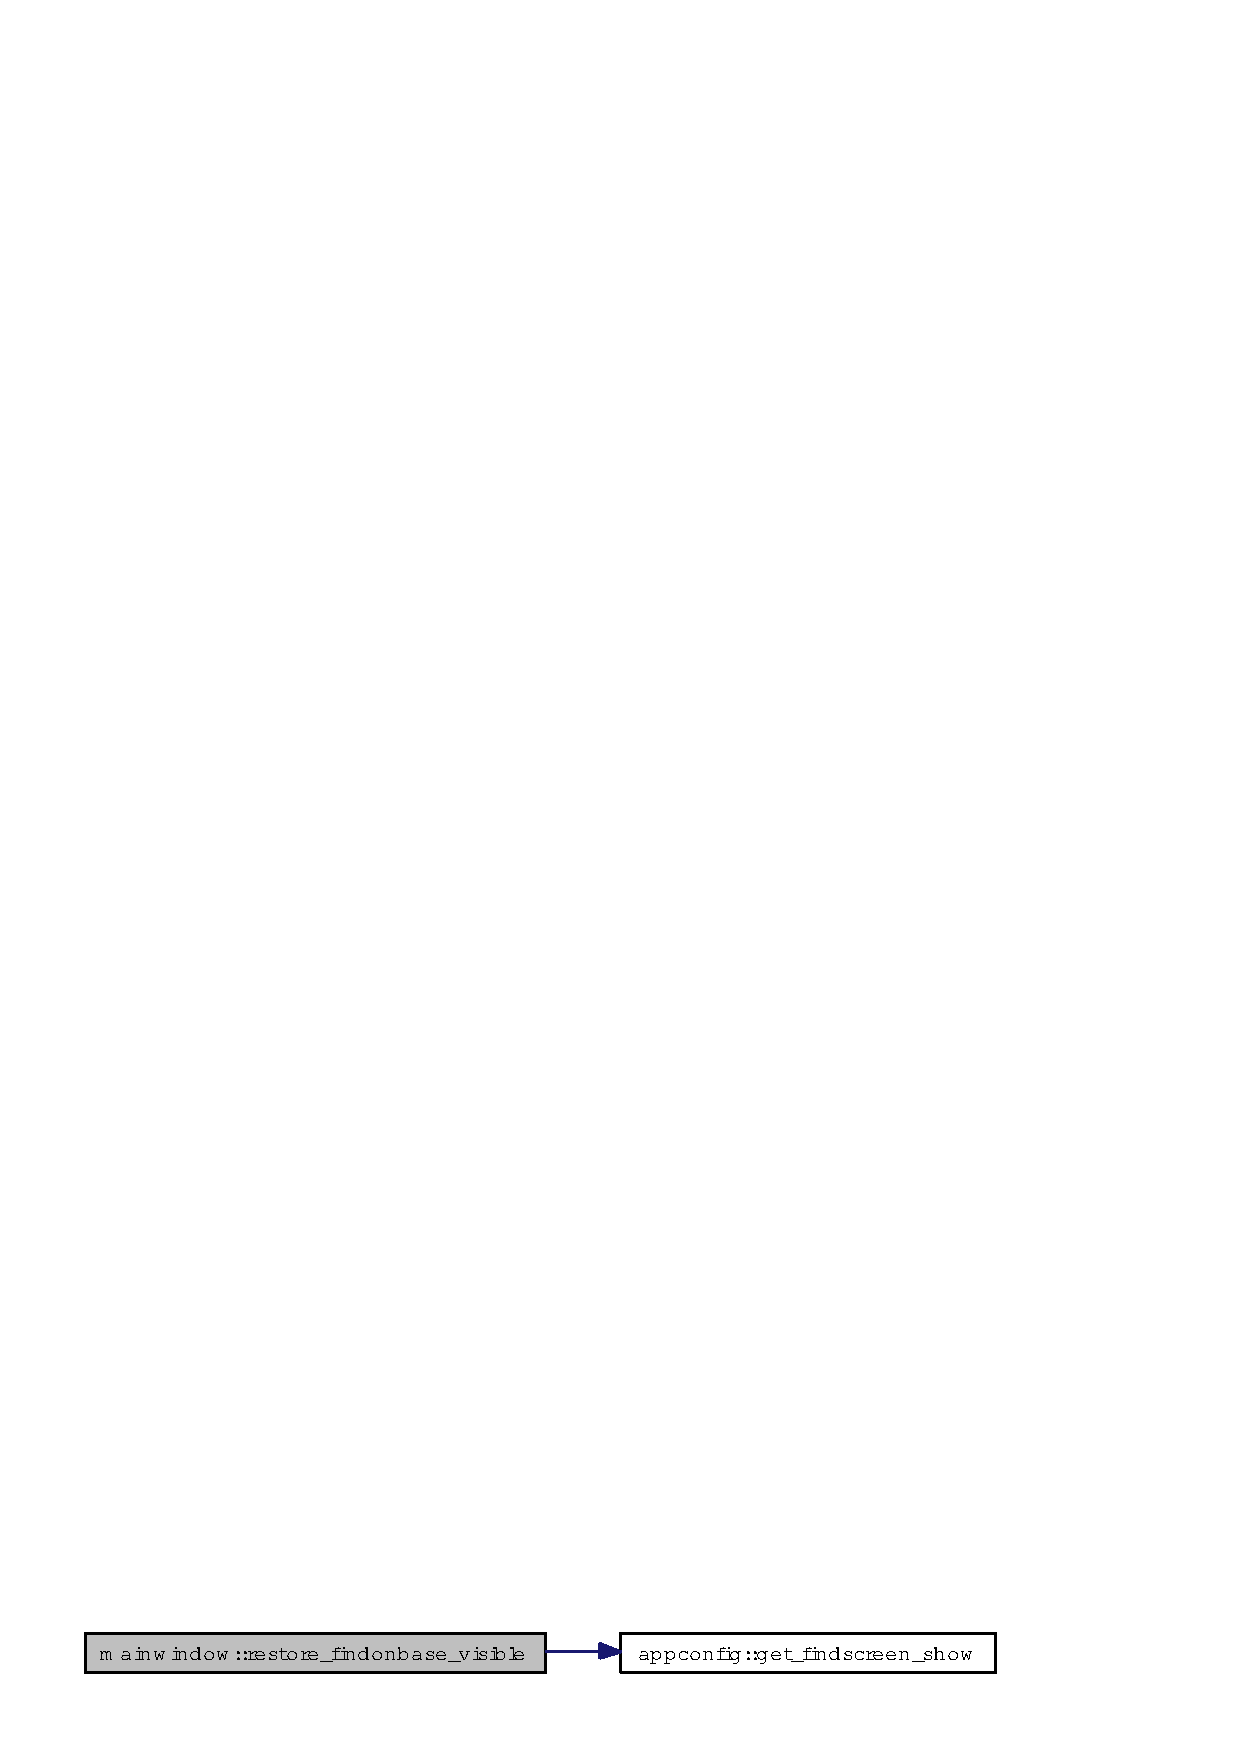
\includegraphics[width=241pt]{classmainwindow_676fda5aa4ca3b8d2d57c4521d69f00b_cgraph}
\end{center}
\end{figure}


Here is the caller graph for this function:\begin{figure}[H]
\begin{center}
\leavevmode
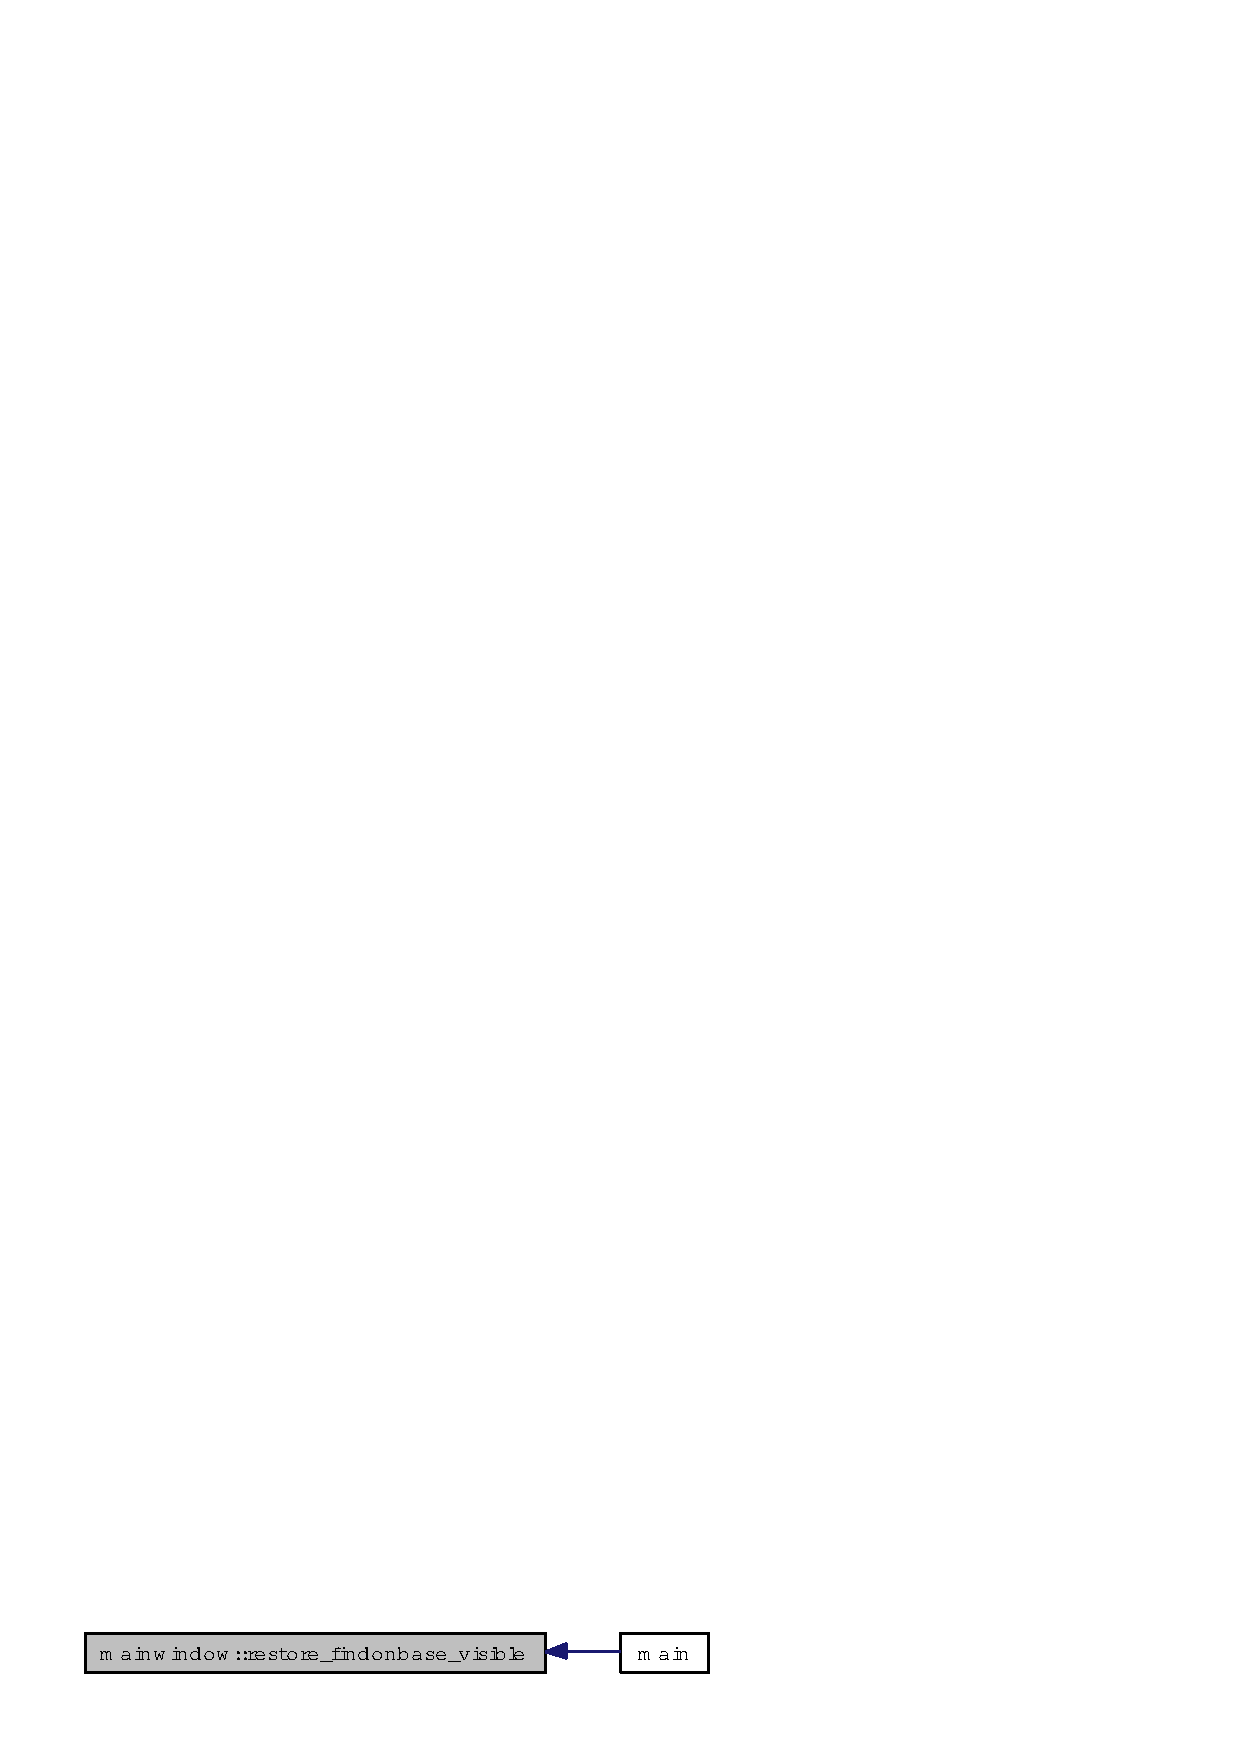
\includegraphics[width=172pt]{classmainwindow_676fda5aa4ca3b8d2d57c4521d69f00b_icgraph}
\end{center}
\end{figure}
\index{mainwindow@{mainwindow}!set_tree_position@{set\_\-tree\_\-position}}
\index{set_tree_position@{set\_\-tree\_\-position}!mainwindow@{mainwindow}}
\subsubsection{\setlength{\rightskip}{0pt plus 5cm}void mainwindow::set\_\-tree\_\-position (QString\-List {\em path})}\label{classmainwindow_1ea5fc01161f568df189d539468a31b5}




Definition at line 146 of file mainwindow.cpp.

References Tree\-Item::data(), knowtreemodel::get\_\-item\_\-index(), Tree\-Model::get\-Item(), treescreen::kntrmodel, treescreen::set\_\-cursor\_\-to\_\-index(), and treeview.

Referenced by restore\_\-tree\_\-position().

Here is the call graph for this function:\begin{figure}[H]
\begin{center}
\leavevmode
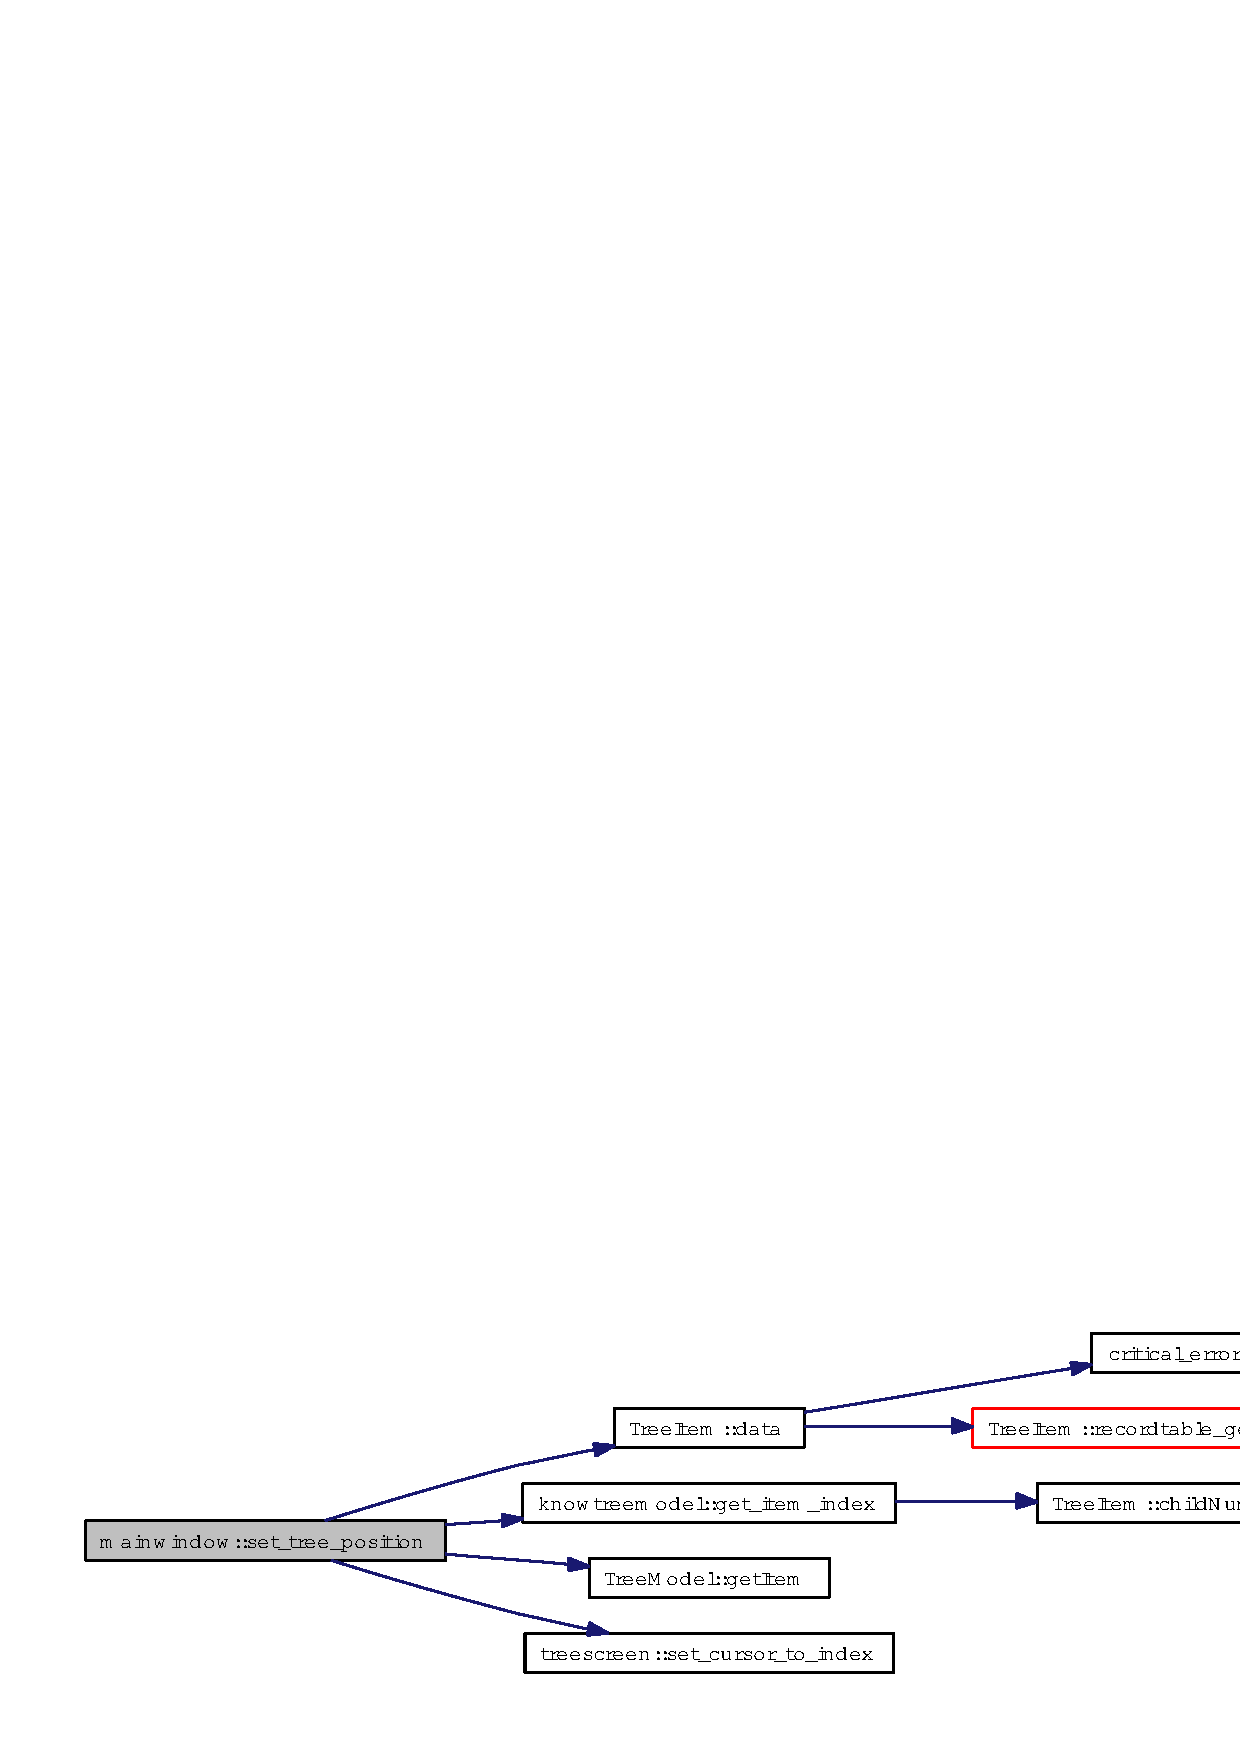
\includegraphics[width=333pt]{classmainwindow_1ea5fc01161f568df189d539468a31b5_cgraph}
\end{center}
\end{figure}


Here is the caller graph for this function:\begin{figure}[H]
\begin{center}
\leavevmode
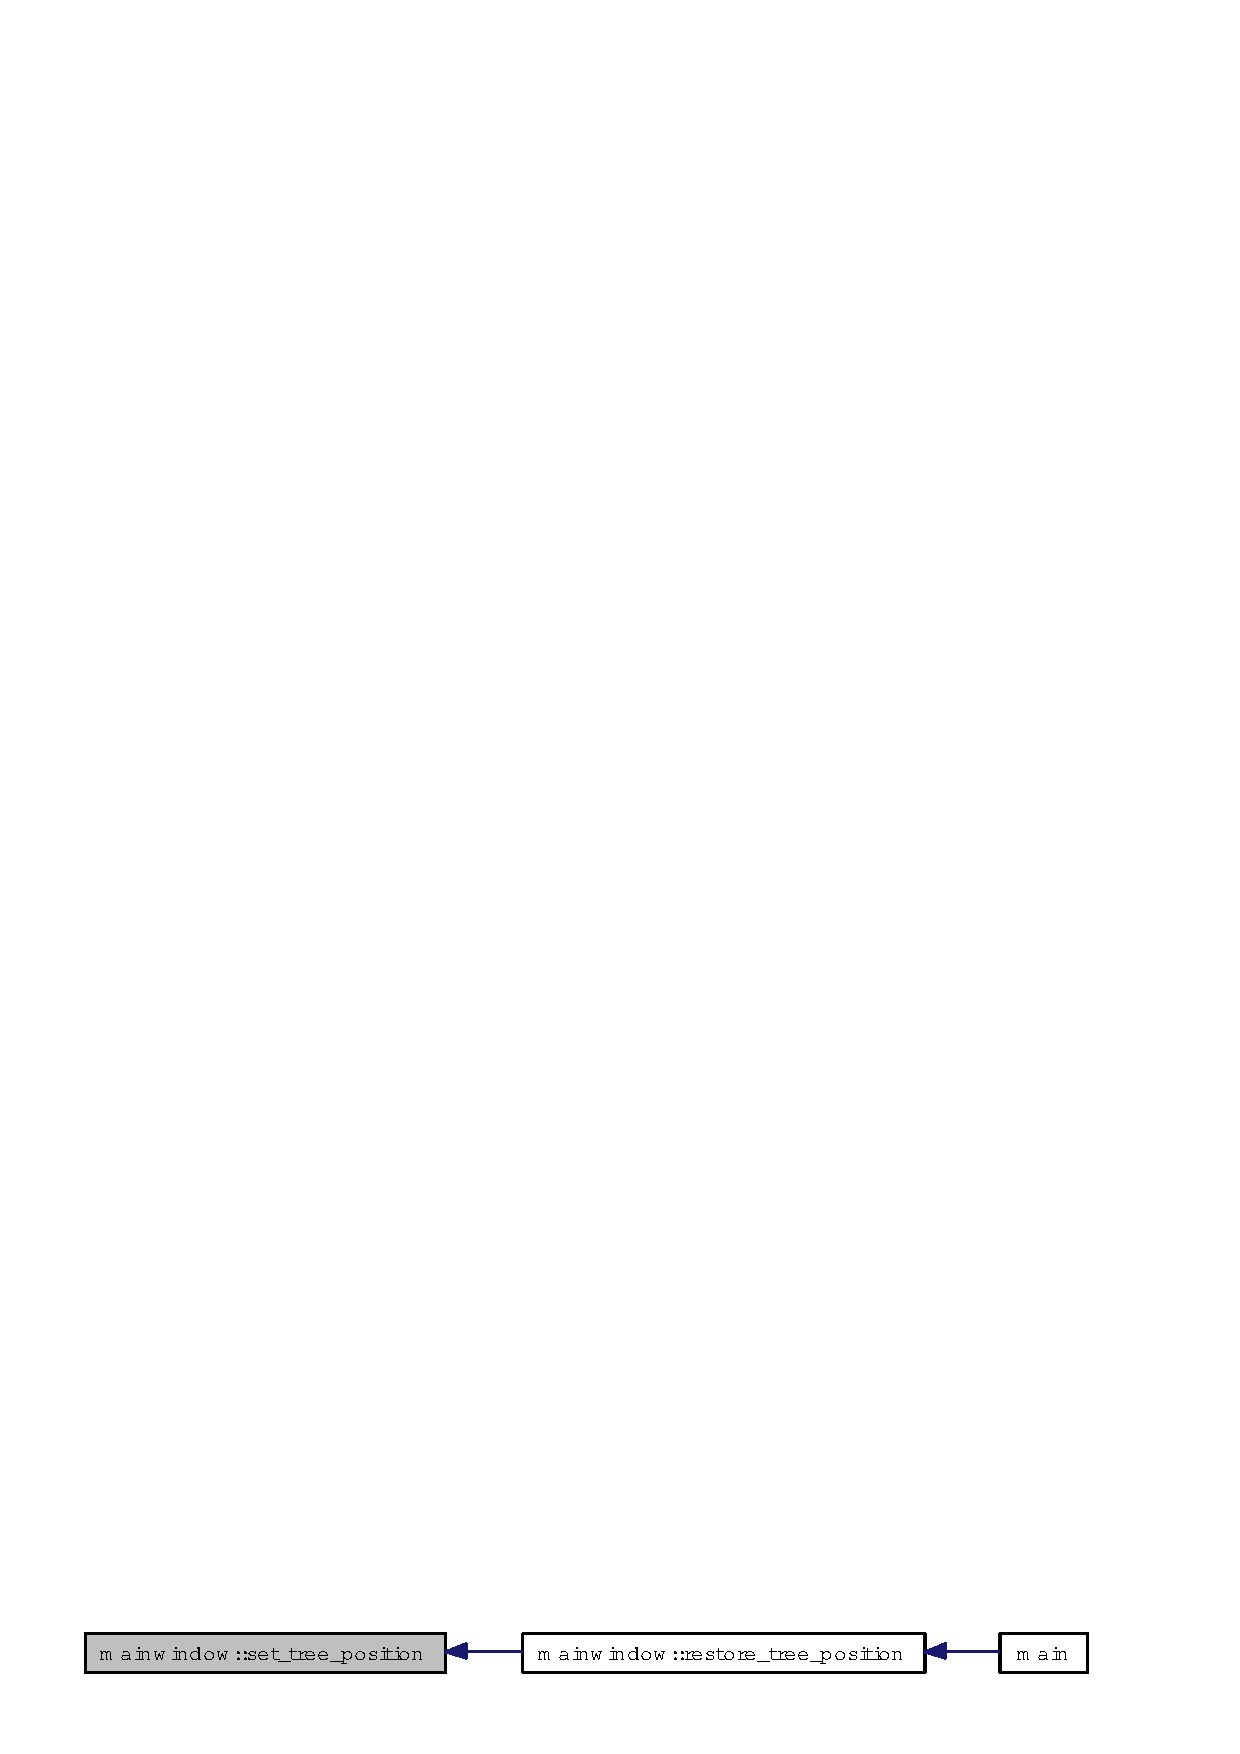
\includegraphics[width=263pt]{classmainwindow_1ea5fc01161f568df189d539468a31b5_icgraph}
\end{center}
\end{figure}
\index{mainwindow@{mainwindow}!set_recordtable_position@{set\_\-recordtable\_\-position}}
\index{set_recordtable_position@{set\_\-recordtable\_\-position}!mainwindow@{mainwindow}}
\subsubsection{\setlength{\rightskip}{0pt plus 5cm}void mainwindow::set\_\-recordtable\_\-position (int {\em n})}\label{classmainwindow_ab31b7cddf7fbd4ab77b90ae46b52fde}




Definition at line 177 of file mainwindow.cpp.

References recordtableview, and recordtablescreen::set\_\-selection\_\-to\_\-pos().

Referenced by restore\_\-recordtable\_\-position().

Here is the call graph for this function:\begin{figure}[H]
\begin{center}
\leavevmode
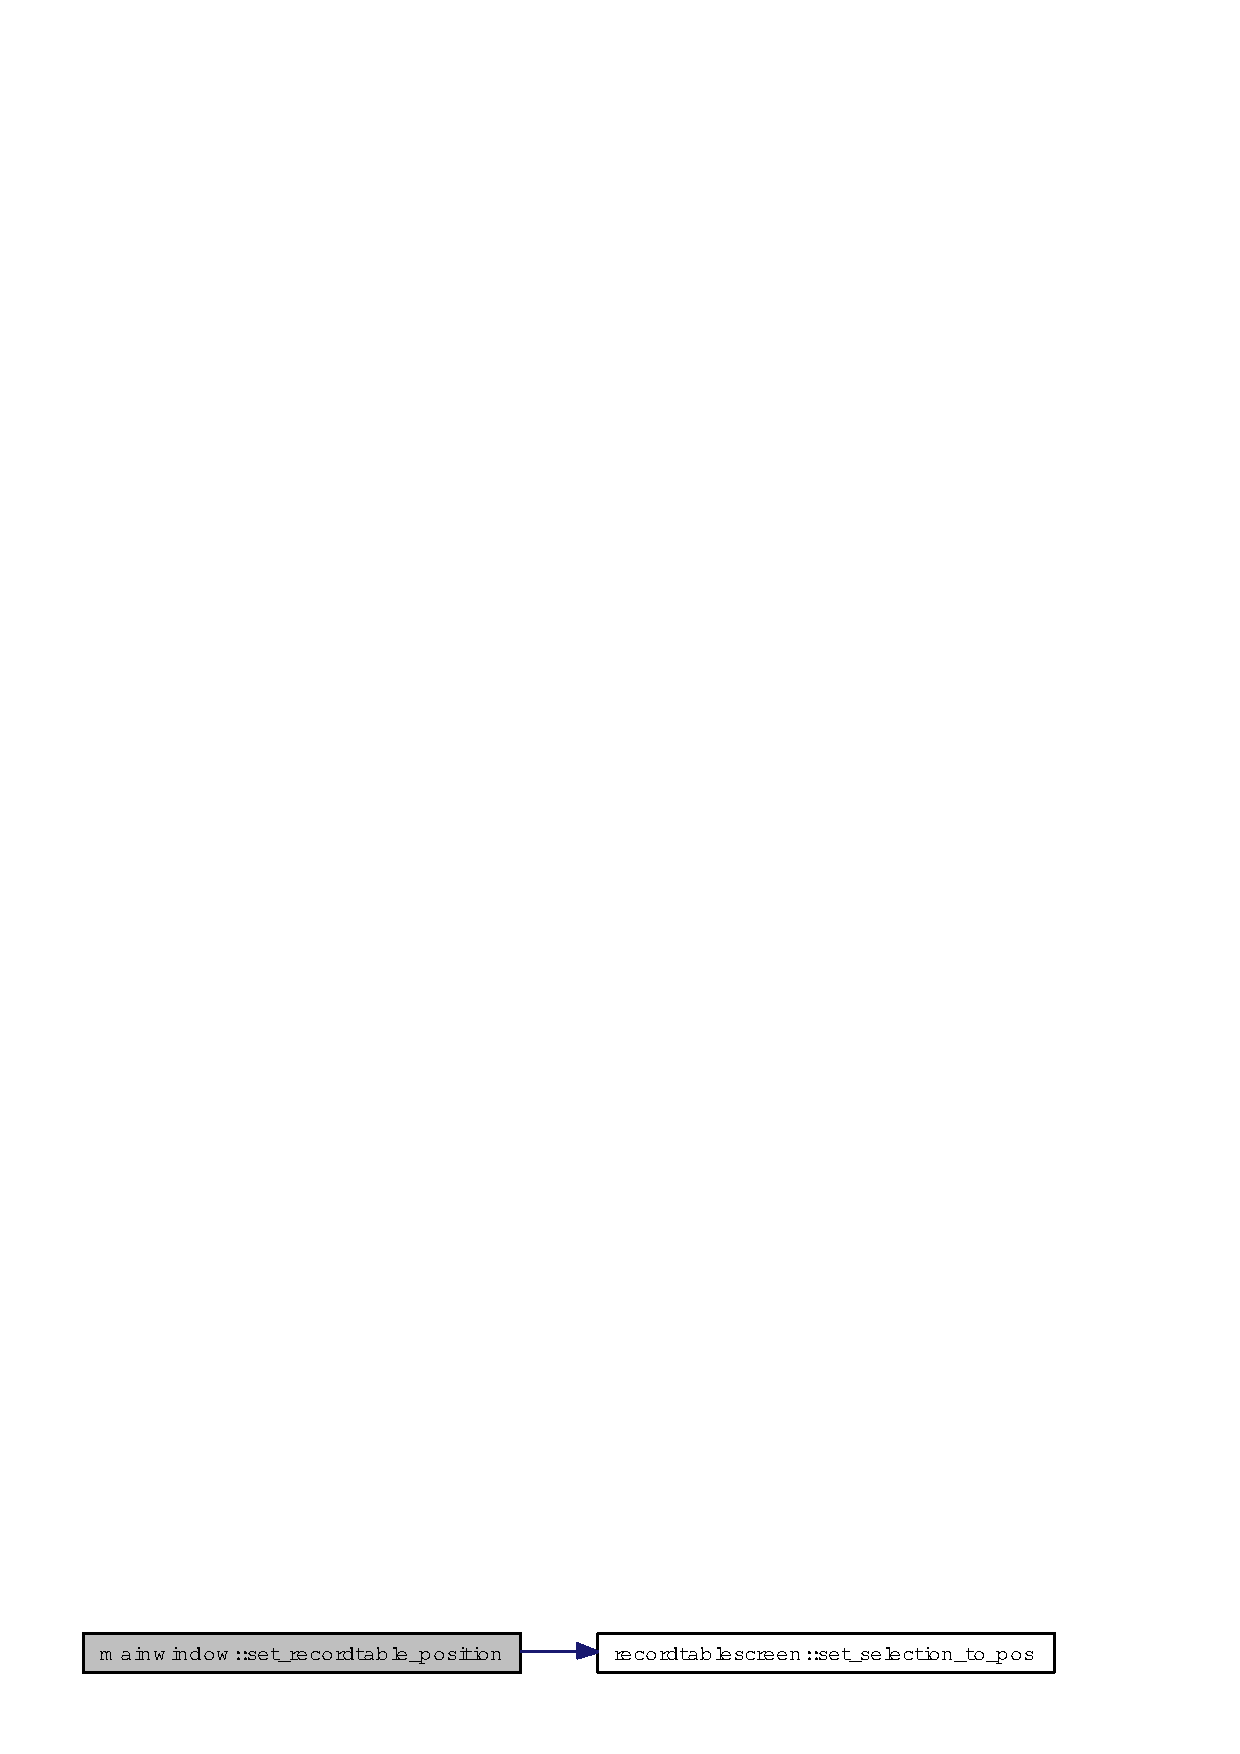
\includegraphics[width=255pt]{classmainwindow_ab31b7cddf7fbd4ab77b90ae46b52fde_cgraph}
\end{center}
\end{figure}


Here is the caller graph for this function:\begin{figure}[H]
\begin{center}
\leavevmode
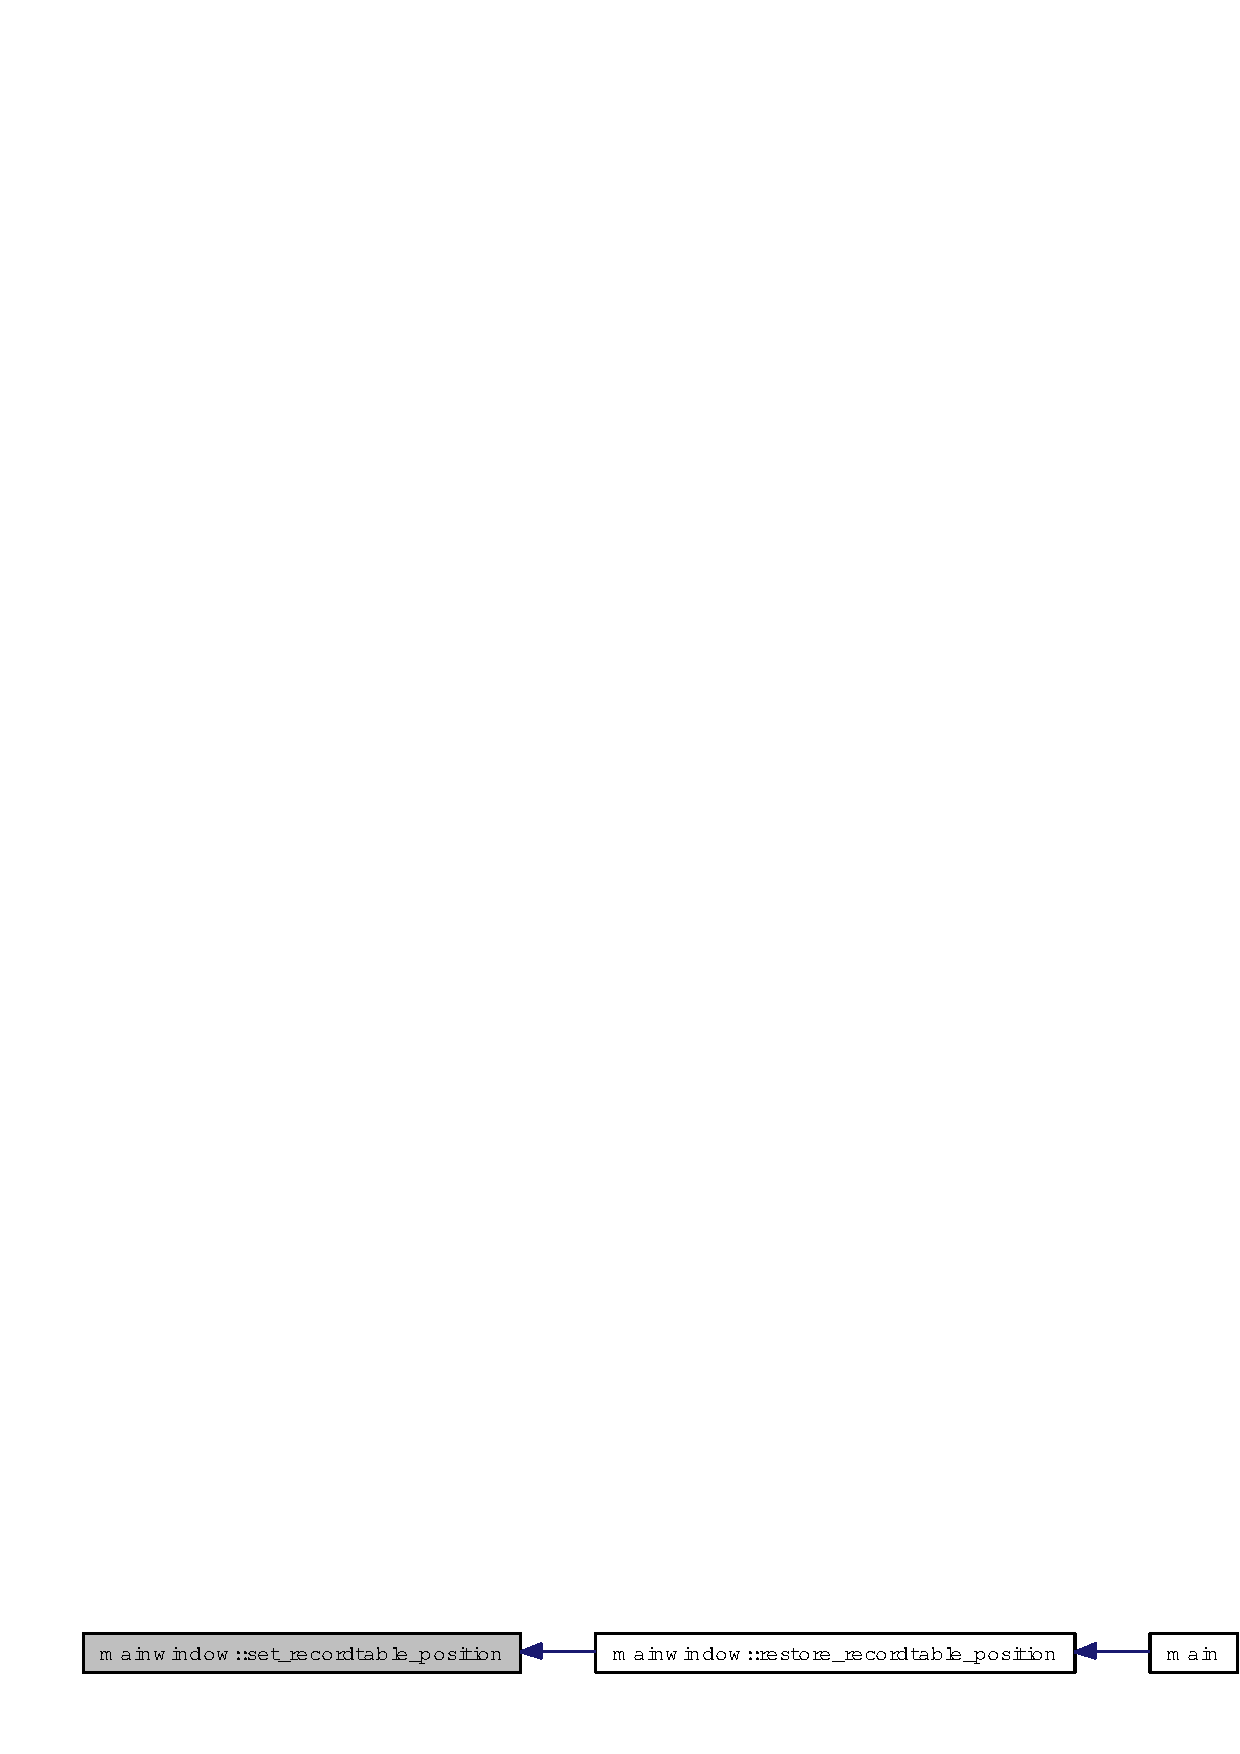
\includegraphics[width=299pt]{classmainwindow_ab31b7cddf7fbd4ab77b90ae46b52fde_icgraph}
\end{center}
\end{figure}
\index{mainwindow@{mainwindow}!fileNew@{fileNew}}
\index{fileNew@{fileNew}!mainwindow@{mainwindow}}
\subsubsection{\setlength{\rightskip}{0pt plus 5cm}void mainwindow::file\-New (void)\hspace{0.3cm}{\tt  [private, slot]}}\label{classmainwindow_7b27eac943c2c3b42b8c1709c08cd160}




Definition at line 264 of file mainwindow.cpp.

Referenced by init\-File\-Actions().\index{mainwindow@{mainwindow}!fileOpen@{fileOpen}}
\index{fileOpen@{fileOpen}!mainwindow@{mainwindow}}
\subsubsection{\setlength{\rightskip}{0pt plus 5cm}void mainwindow::file\-Open (void)\hspace{0.3cm}{\tt  [private, slot]}}\label{classmainwindow_881a54e18200f7b3812f84cb76362322}




Definition at line 270 of file mainwindow.cpp.

Referenced by init\-File\-Actions().\index{mainwindow@{mainwindow}!fileSave@{fileSave}}
\index{fileSave@{fileSave}!mainwindow@{mainwindow}}
\subsubsection{\setlength{\rightskip}{0pt plus 5cm}bool mainwindow::file\-Save (void)\hspace{0.3cm}{\tt  [private, slot]}}\label{classmainwindow_266ed66c32e6c31a329fe64cefac8bab}




Definition at line 276 of file mainwindow.cpp.

Referenced by init\-File\-Actions().\index{mainwindow@{mainwindow}!fileSaveAs@{fileSaveAs}}
\index{fileSaveAs@{fileSaveAs}!mainwindow@{mainwindow}}
\subsubsection{\setlength{\rightskip}{0pt plus 5cm}bool mainwindow::file\-Save\-As (void)\hspace{0.3cm}{\tt  [private, slot]}}\label{classmainwindow_2fe00a916b7e48fa9fef40d8032eac6b}




Definition at line 282 of file mainwindow.cpp.

Referenced by init\-File\-Actions().\index{mainwindow@{mainwindow}!filePrint@{filePrint}}
\index{filePrint@{filePrint}!mainwindow@{mainwindow}}
\subsubsection{\setlength{\rightskip}{0pt plus 5cm}void mainwindow::file\-Print (void)\hspace{0.3cm}{\tt  [private, slot]}}\label{classmainwindow_dfd16a7e4ae01e08bb546388f9cf969d}




Definition at line 288 of file mainwindow.cpp.

References editorview, and editor::textarea.

Referenced by init\-File\-Actions().\index{mainwindow@{mainwindow}!filePrintPreview@{filePrintPreview}}
\index{filePrintPreview@{filePrintPreview}!mainwindow@{mainwindow}}
\subsubsection{\setlength{\rightskip}{0pt plus 5cm}void mainwindow::file\-Print\-Preview (void)\hspace{0.3cm}{\tt  [private, slot]}}\label{classmainwindow_388d5a83b09b316d9633546d26e15fb4}




Definition at line 303 of file mainwindow.cpp.

References editorview, and editor::textarea.

Referenced by init\-File\-Actions().\index{mainwindow@{mainwindow}!filePrintPdf@{filePrintPdf}}
\index{filePrintPdf@{filePrintPdf}!mainwindow@{mainwindow}}
\subsubsection{\setlength{\rightskip}{0pt plus 5cm}void mainwindow::file\-Print\-Pdf (void)\hspace{0.3cm}{\tt  [private, slot]}}\label{classmainwindow_5f7a78c602919a7ca92aae56532b4ed5}




Definition at line 311 of file mainwindow.cpp.

References editorview, and editor::textarea.

Referenced by init\-File\-Actions().\index{mainwindow@{mainwindow}!icon_activated@{icon\_\-activated}}
\index{icon_activated@{icon\_\-activated}!mainwindow@{mainwindow}}
\subsubsection{\setlength{\rightskip}{0pt plus 5cm}void mainwindow::icon\_\-activated (QSystem\-Tray\-Icon::Activation\-Reason {\em reason})\hspace{0.3cm}{\tt  [private, slot]}}\label{classmainwindow_3c050e01ff3cd4abda990c47807a6327}




Definition at line 378 of file mainwindow.cpp.

Referenced by set\_\-icon().\index{mainwindow@{mainwindow}!application_exit@{application\_\-exit}}
\index{application_exit@{application\_\-exit}!mainwindow@{mainwindow}}
\subsubsection{\setlength{\rightskip}{0pt plus 5cm}void mainwindow::application\_\-exit (void)\hspace{0.3cm}{\tt  [private, slot]}}\label{classmainwindow_2a9e00901bfba97614e2b80b37cb02db}




Definition at line 328 of file mainwindow.cpp.

Referenced by init\-File\-Actions().\index{mainwindow@{mainwindow}!setup_ui@{setup\_\-ui}}
\index{setup_ui@{setup\_\-ui}!mainwindow@{mainwindow}}
\subsubsection{\setlength{\rightskip}{0pt plus 5cm}void mainwindow::setup\_\-ui (void)\hspace{0.3cm}{\tt  [private]}}\label{classmainwindow_f3d64dde81a35e22564d154736152b00}




Definition at line 43 of file mainwindow.cpp.

References editorview, findscreendisp, recordtableview, statbar, and treeview.

Referenced by mainwindow().

Here is the caller graph for this function:\begin{figure}[H]
\begin{center}
\leavevmode
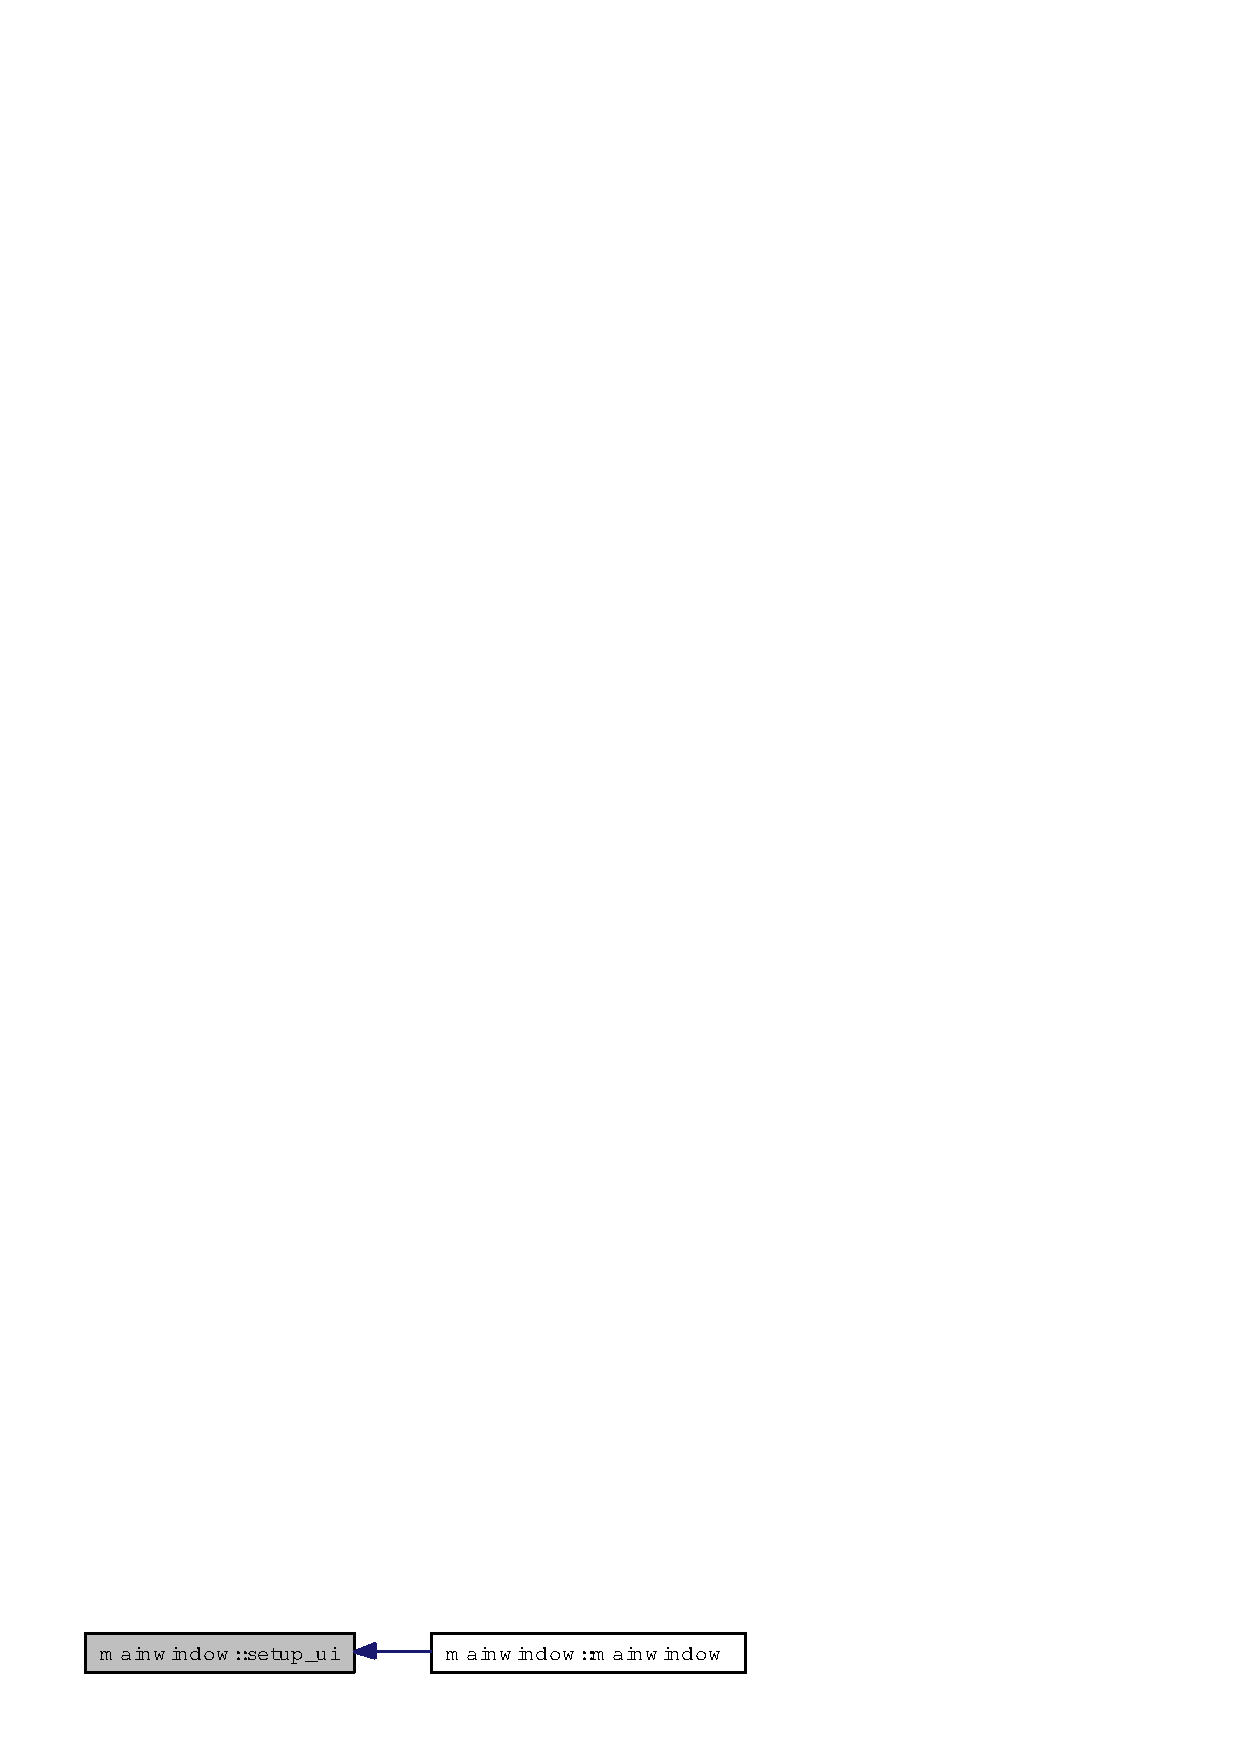
\includegraphics[width=181pt]{classmainwindow_f3d64dde81a35e22564d154736152b00_icgraph}
\end{center}
\end{figure}
\index{mainwindow@{mainwindow}!setup_signals@{setup\_\-signals}}
\index{setup_signals@{setup\_\-signals}!mainwindow@{mainwindow}}
\subsubsection{\setlength{\rightskip}{0pt plus 5cm}void mainwindow::setup\_\-signals (void)\hspace{0.3cm}{\tt  [private]}}\label{classmainwindow_9e1c0ddaa70c6851ea20983c36adb52b}




Definition at line 64 of file mainwindow.cpp.

Referenced by mainwindow().

Here is the caller graph for this function:\begin{figure}[H]
\begin{center}
\leavevmode
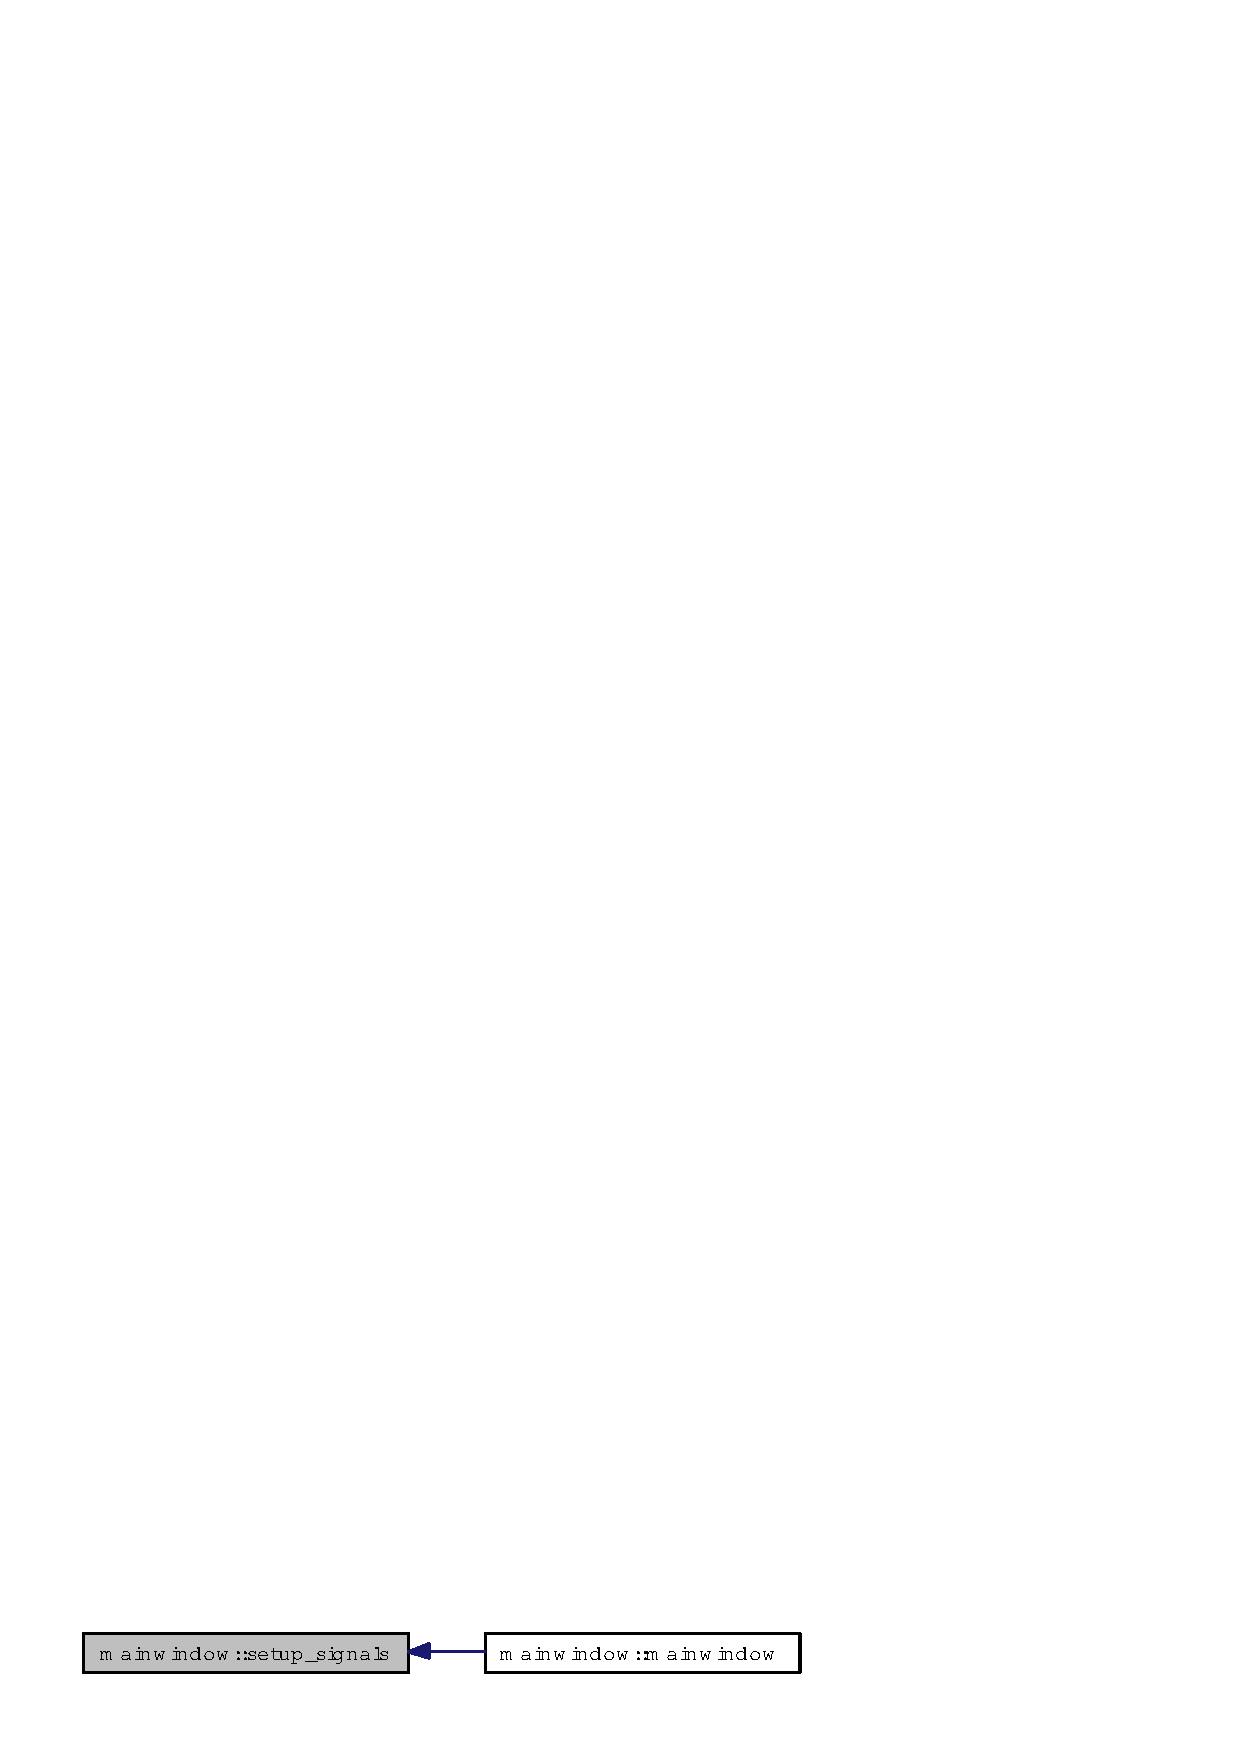
\includegraphics[width=194pt]{classmainwindow_9e1c0ddaa70c6851ea20983c36adb52b_icgraph}
\end{center}
\end{figure}
\index{mainwindow@{mainwindow}!assembly@{assembly}}
\index{assembly@{assembly}!mainwindow@{mainwindow}}
\subsubsection{\setlength{\rightskip}{0pt plus 5cm}void mainwindow::assembly (void)\hspace{0.3cm}{\tt  [private]}}\label{classmainwindow_f166528e596f9615d5ecd3a8d545ef9b}




Definition at line 70 of file mainwindow.cpp.

References editorview, findscreendisp, findsplitter, hspl, recordtableview, treeview, and vspl.

Referenced by mainwindow().

Here is the caller graph for this function:\begin{figure}[H]
\begin{center}
\leavevmode
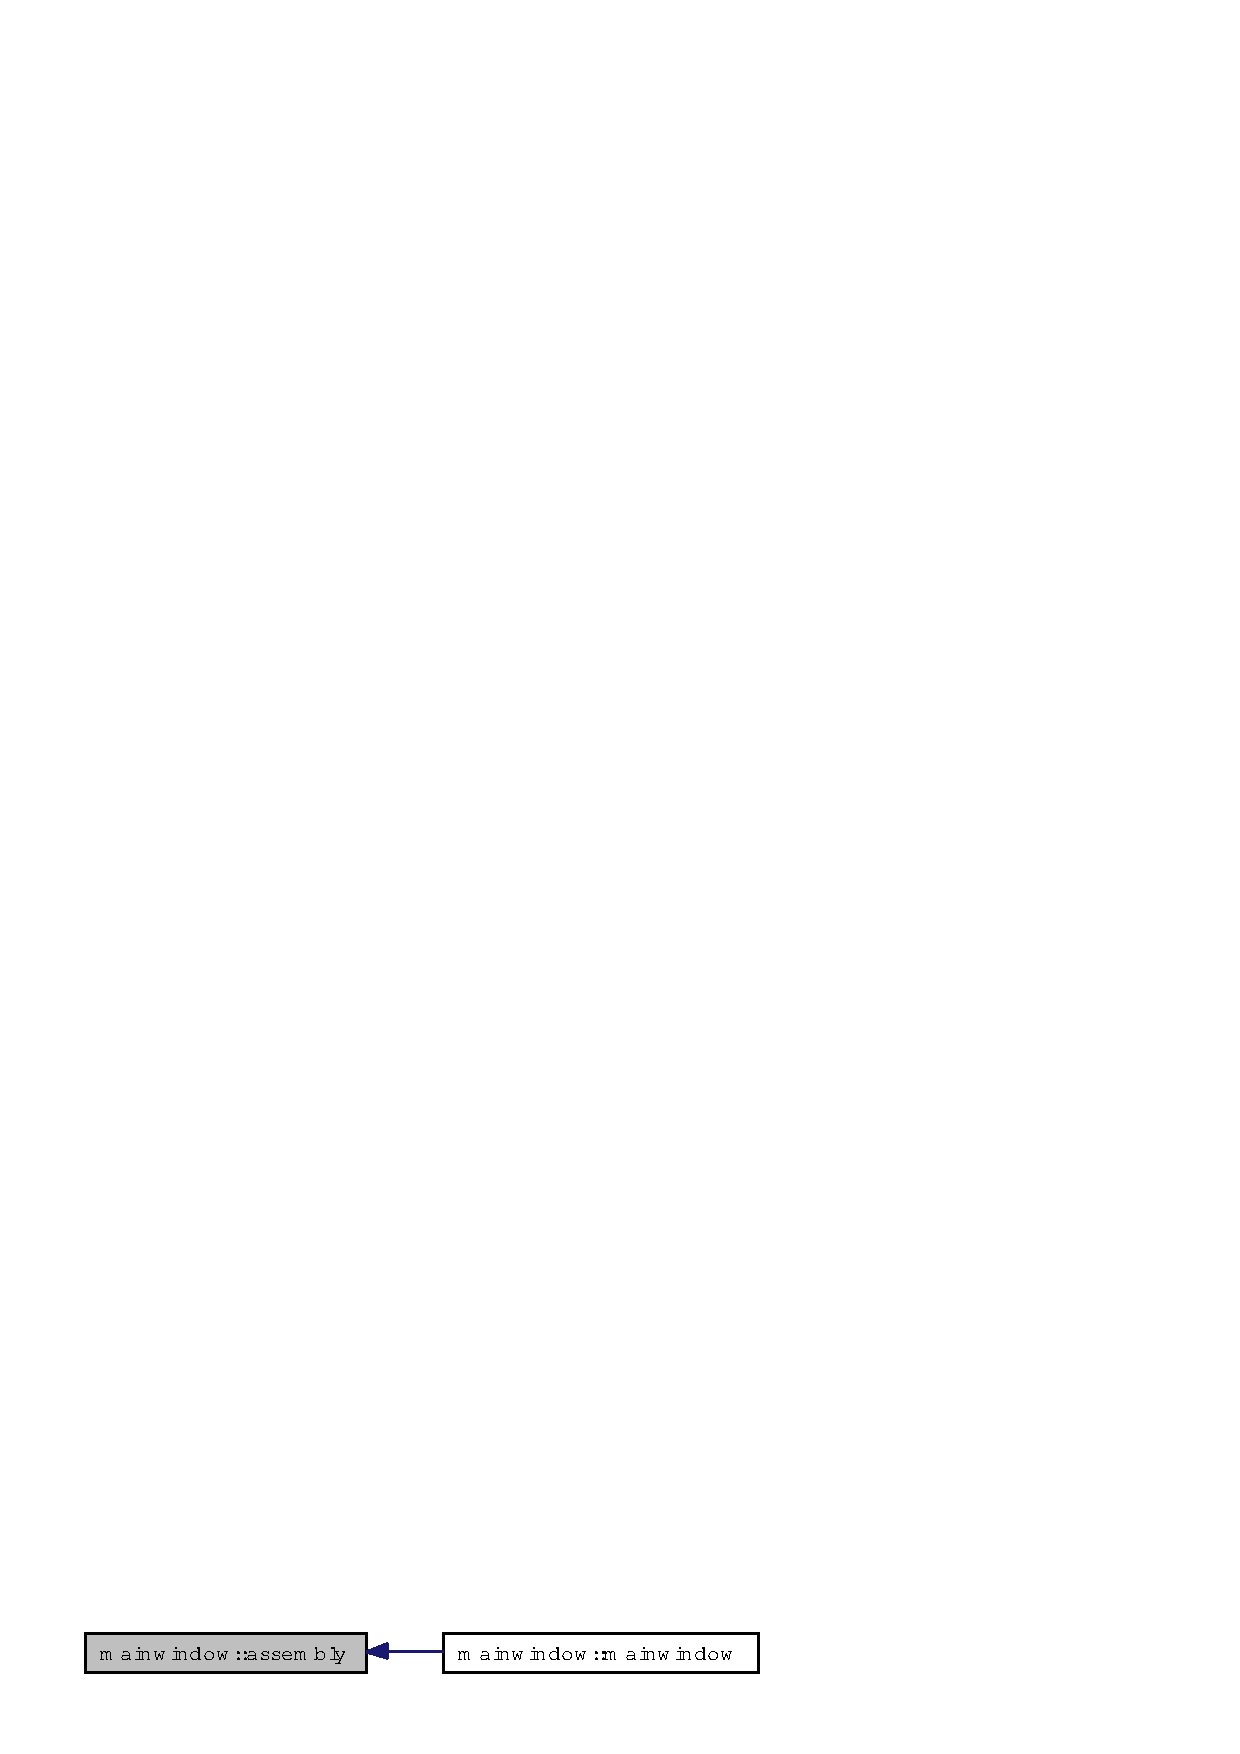
\includegraphics[width=184pt]{classmainwindow_f166528e596f9615d5ecd3a8d545ef9b_icgraph}
\end{center}
\end{figure}
\index{mainwindow@{mainwindow}!initFileActions@{initFileActions}}
\index{initFileActions@{initFileActions}!mainwindow@{mainwindow}}
\subsubsection{\setlength{\rightskip}{0pt plus 5cm}void mainwindow::init\-File\-Actions (void)\hspace{0.3cm}{\tt  [private]}}\label{classmainwindow_c2cf8262152cac2a283474c3f42a22ac}




Definition at line 198 of file mainwindow.cpp.

References application\_\-exit(), file\-New(), file\-Open(), file\-Print(), file\-Print\-Pdf(), file\-Print\-Preview(), file\-Save(), and file\-Save\-As().

Referenced by mainwindow().

Here is the caller graph for this function:\begin{figure}[H]
\begin{center}
\leavevmode
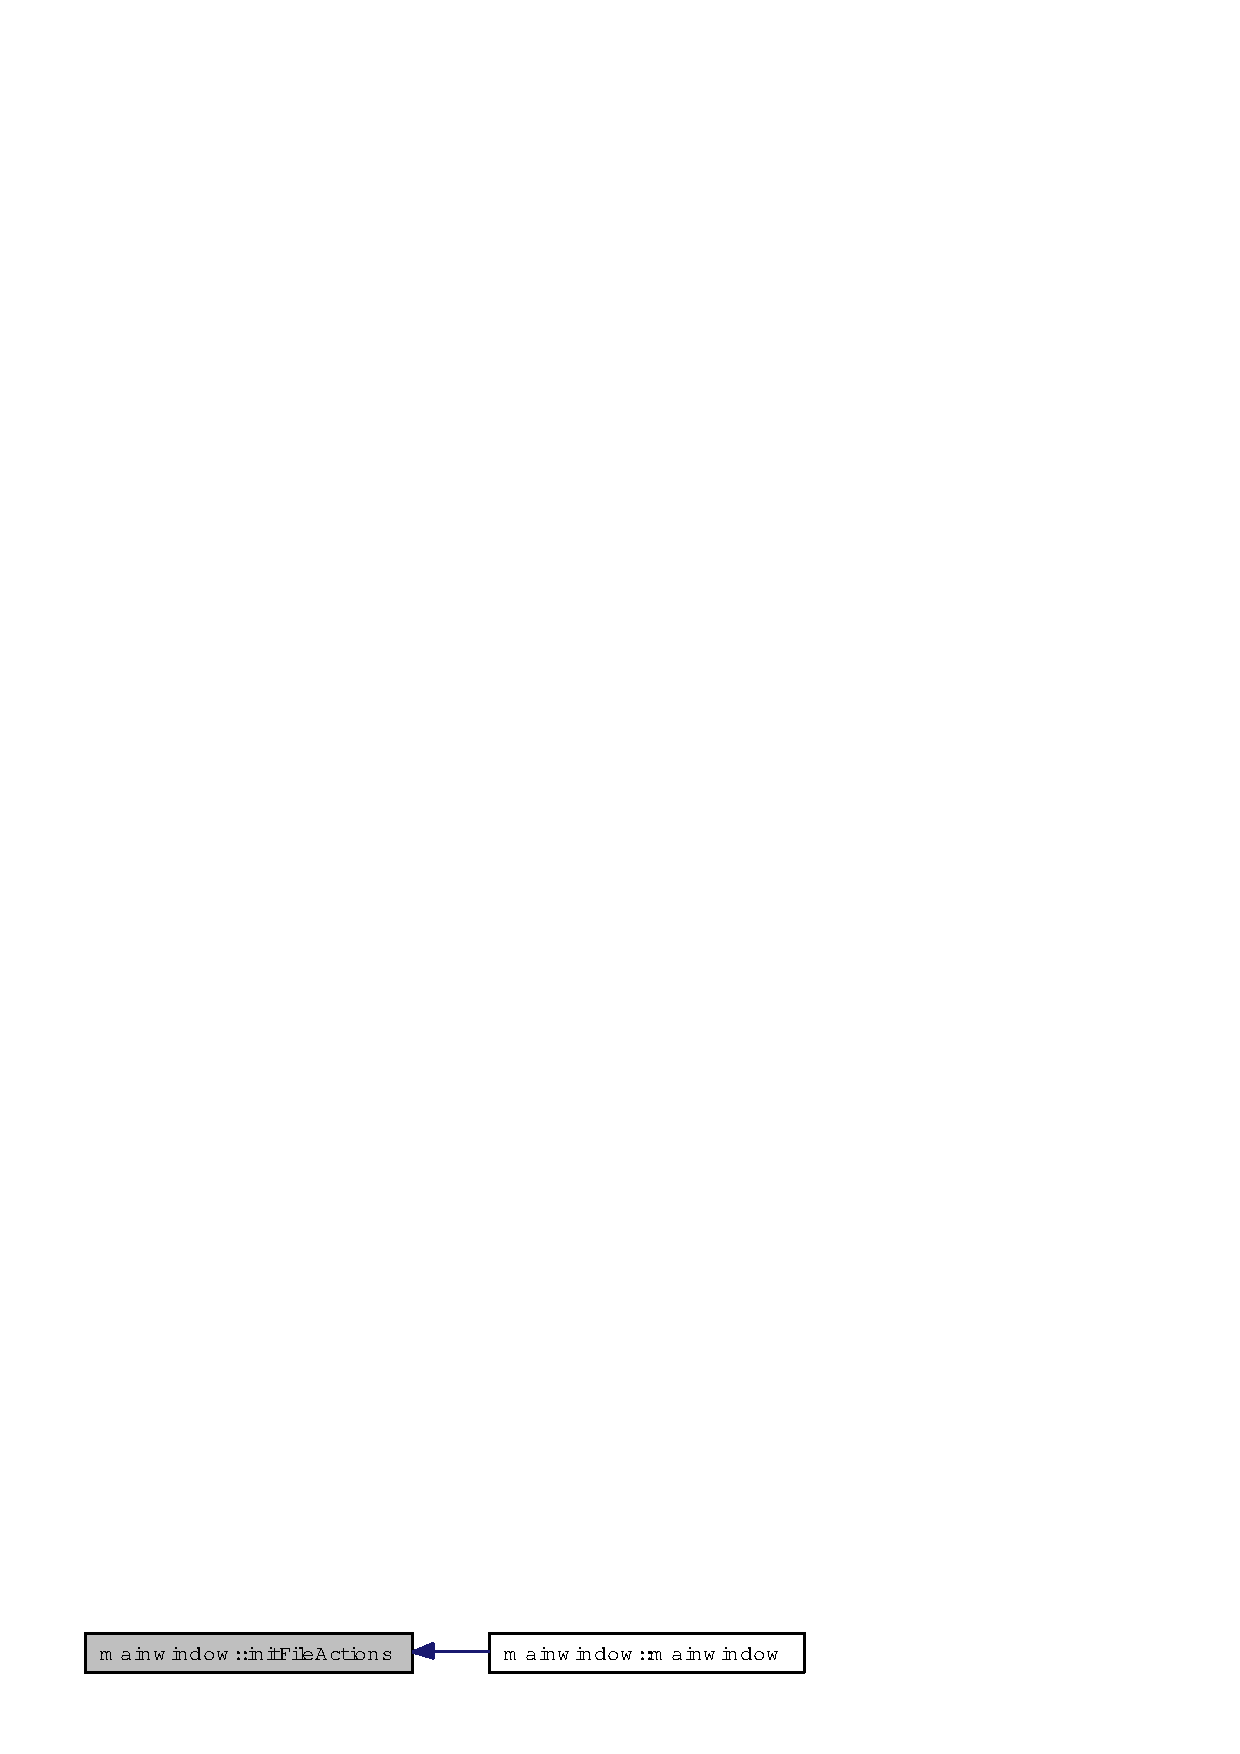
\includegraphics[width=195pt]{classmainwindow_c2cf8262152cac2a283474c3f42a22ac_icgraph}
\end{center}
\end{figure}
\index{mainwindow@{mainwindow}!initRecordTableActions@{initRecordTableActions}}
\index{initRecordTableActions@{initRecordTableActions}!mainwindow@{mainwindow}}
\subsubsection{\setlength{\rightskip}{0pt plus 5cm}void mainwindow::init\-Record\-Table\-Actions (void)\hspace{0.3cm}{\tt  [private]}}\label{classmainwindow_c745dbade81fb969eab44d79079e05b8}


\index{mainwindow@{mainwindow}!setup_icon_actions@{setup\_\-icon\_\-actions}}
\index{setup_icon_actions@{setup\_\-icon\_\-actions}!mainwindow@{mainwindow}}
\subsubsection{\setlength{\rightskip}{0pt plus 5cm}void mainwindow::setup\_\-icon\_\-actions (void)\hspace{0.3cm}{\tt  [private]}}\label{classmainwindow_bc75931596e1d8d8a796291258f9925d}




Definition at line 334 of file mainwindow.cpp.

References tray\_\-maximize\_\-action, tray\_\-minimize\_\-action, tray\_\-quit\_\-action, and tray\_\-restore\_\-action.

Referenced by mainwindow().

Here is the caller graph for this function:\begin{figure}[H]
\begin{center}
\leavevmode
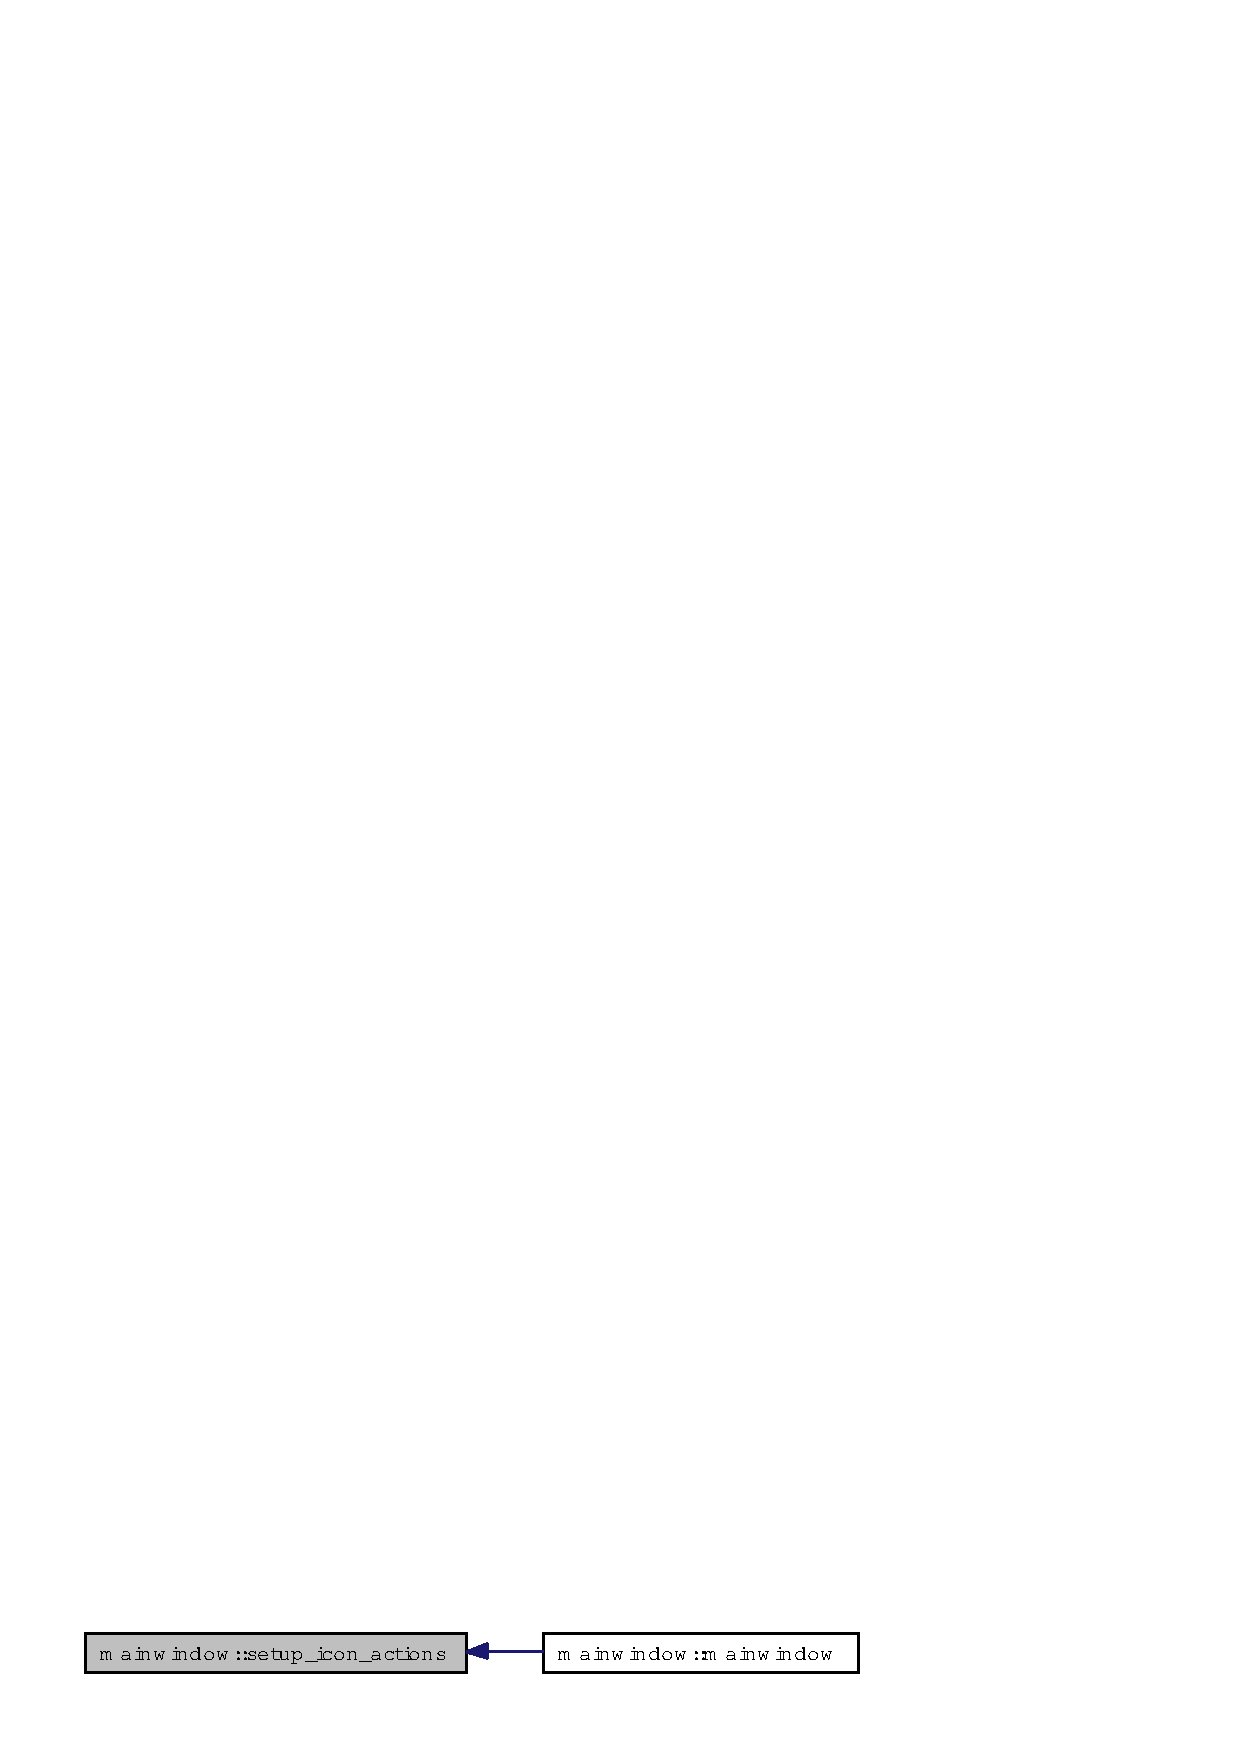
\includegraphics[width=208pt]{classmainwindow_bc75931596e1d8d8a796291258f9925d_icgraph}
\end{center}
\end{figure}
\index{mainwindow@{mainwindow}!create_tray_icon@{create\_\-tray\_\-icon}}
\index{create_tray_icon@{create\_\-tray\_\-icon}!mainwindow@{mainwindow}}
\subsubsection{\setlength{\rightskip}{0pt plus 5cm}void mainwindow::create\_\-tray\_\-icon (void)\hspace{0.3cm}{\tt  [private]}}\label{classmainwindow_e8ef2197826595169fbebe9622afa8ec}




Definition at line 350 of file mainwindow.cpp.

References tray\_\-icon, tray\_\-icon\_\-menu, tray\_\-maximize\_\-action, tray\_\-minimize\_\-action, tray\_\-quit\_\-action, and tray\_\-restore\_\-action.

Referenced by mainwindow().

Here is the caller graph for this function:\begin{figure}[H]
\begin{center}
\leavevmode
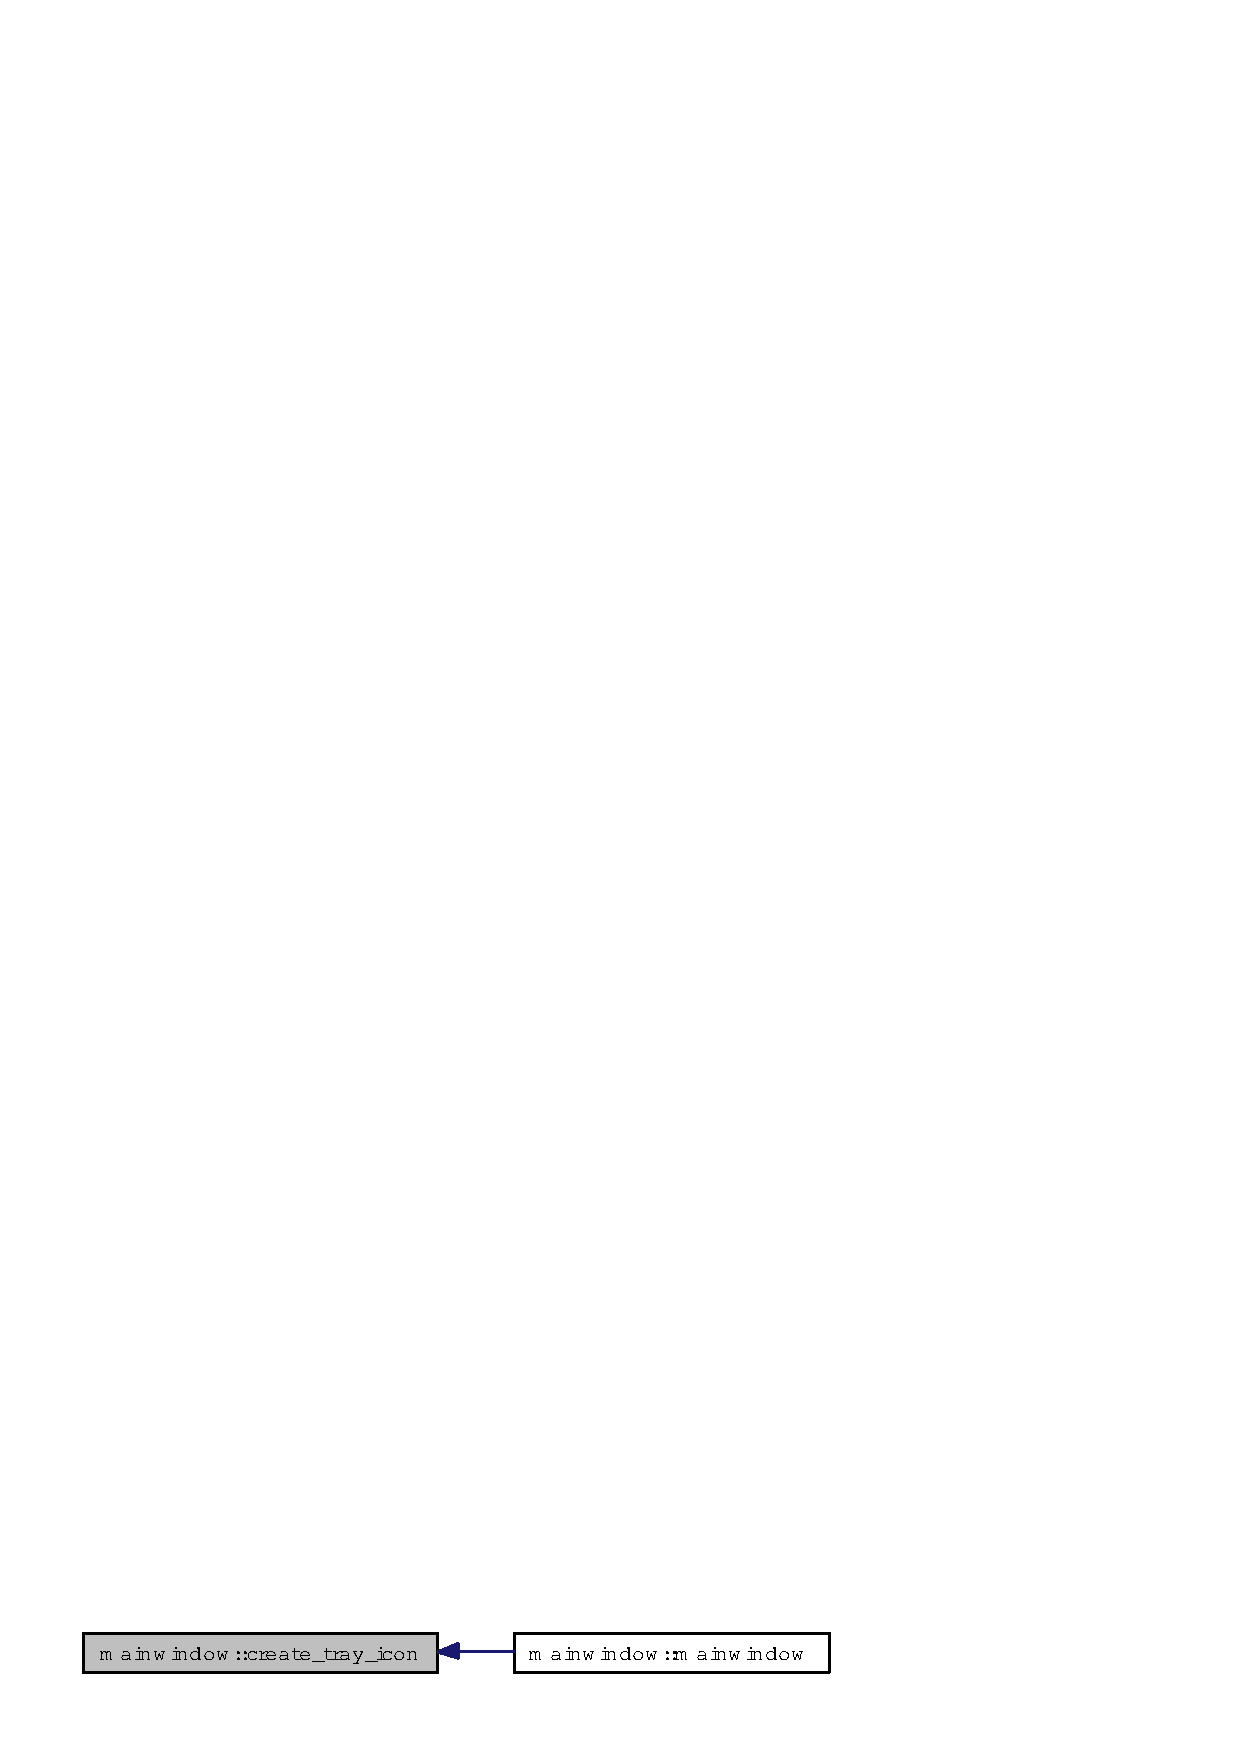
\includegraphics[width=201pt]{classmainwindow_e8ef2197826595169fbebe9622afa8ec_icgraph}
\end{center}
\end{figure}
\index{mainwindow@{mainwindow}!set_icon@{set\_\-icon}}
\index{set_icon@{set\_\-icon}!mainwindow@{mainwindow}}
\subsubsection{\setlength{\rightskip}{0pt plus 5cm}void mainwindow::set\_\-icon (void)\hspace{0.3cm}{\tt  [private]}}\label{classmainwindow_3b071c89ed28b35cbaa1dc815c4a836a}




Definition at line 364 of file mainwindow.cpp.

References icon\_\-activated(), and tray\_\-icon.

Referenced by mainwindow().

Here is the caller graph for this function:\begin{figure}[H]
\begin{center}
\leavevmode
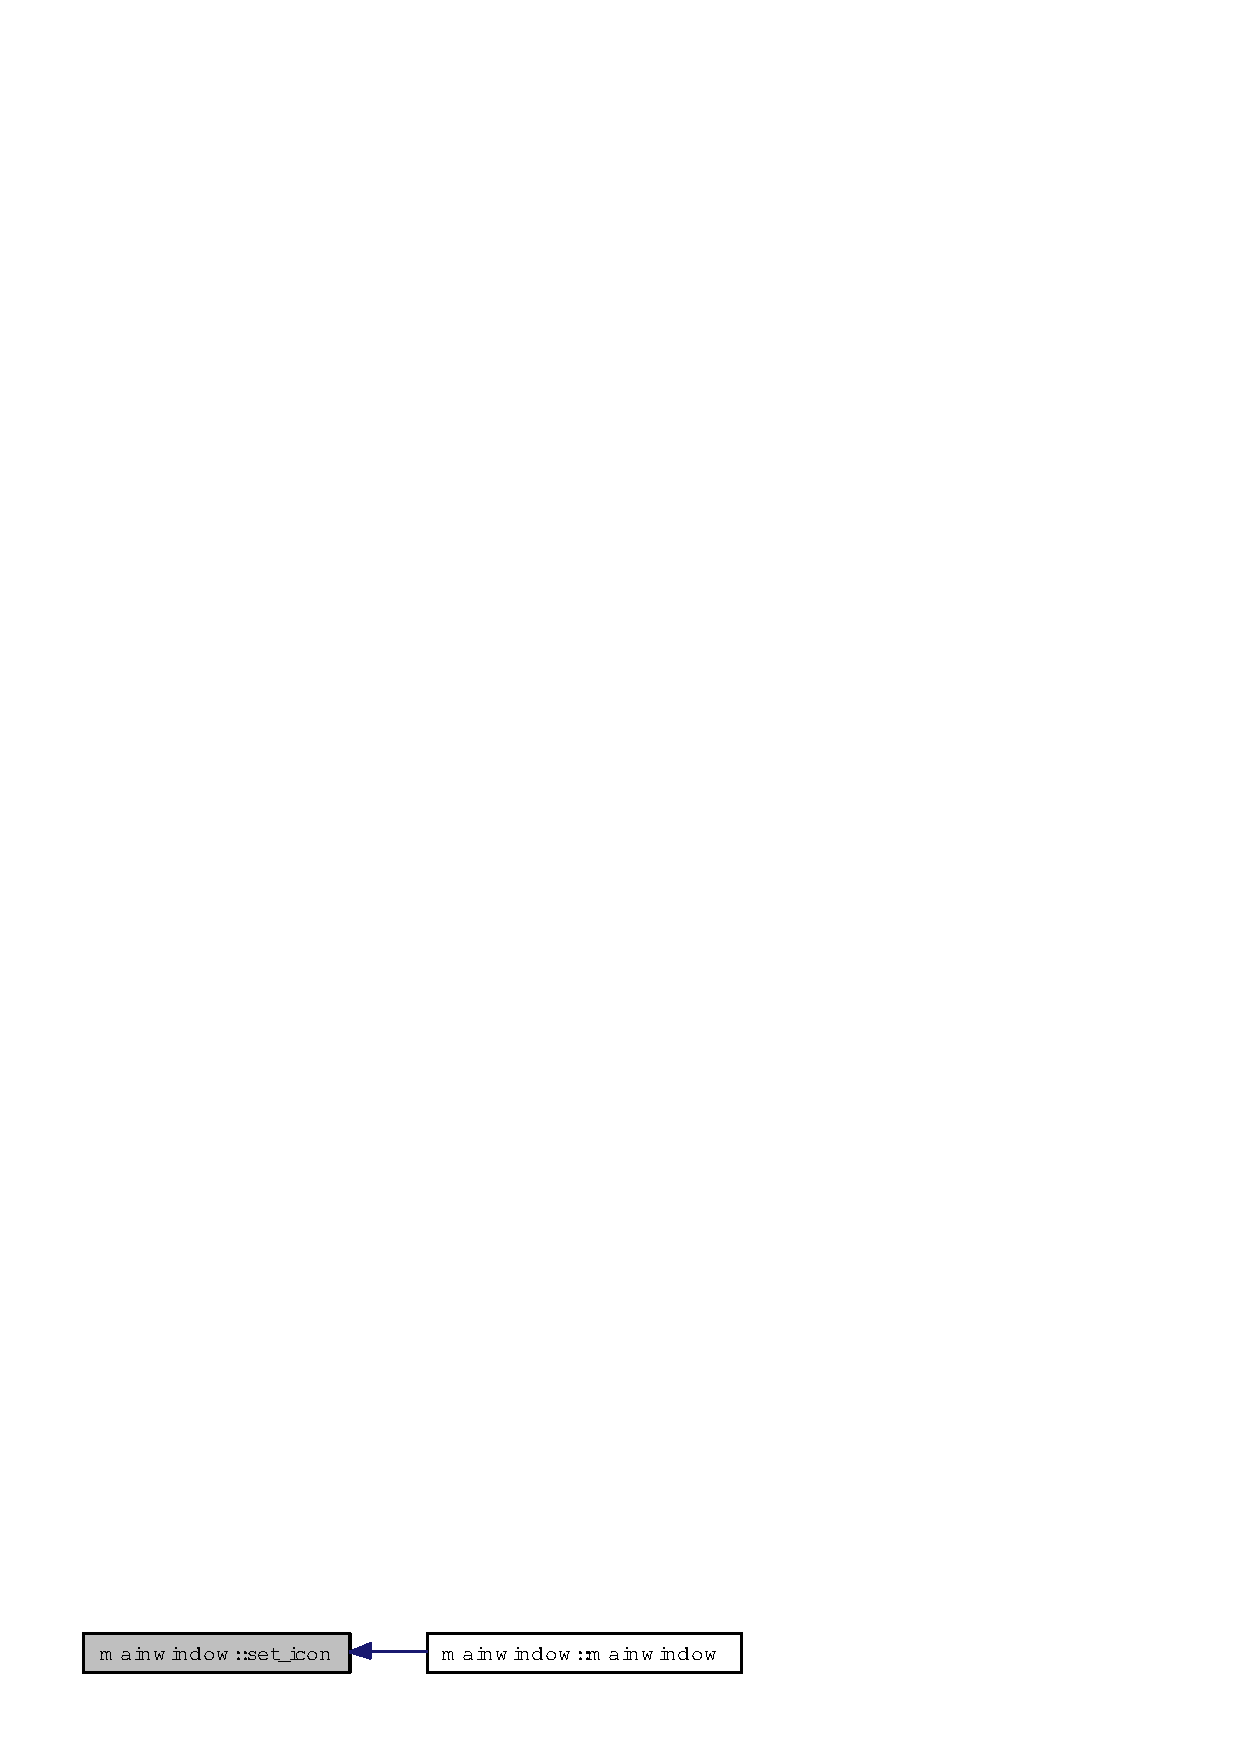
\includegraphics[width=180pt]{classmainwindow_3b071c89ed28b35cbaa1dc815c4a836a_icgraph}
\end{center}
\end{figure}
\index{mainwindow@{mainwindow}!save_geometry@{save\_\-geometry}}
\index{save_geometry@{save\_\-geometry}!mainwindow@{mainwindow}}
\subsubsection{\setlength{\rightskip}{0pt plus 5cm}void mainwindow::save\_\-geometry (void)\hspace{0.3cm}{\tt  [private]}}\label{classmainwindow_129c1ed40a92e5bbc43a7af90575ab6c}




Definition at line 109 of file mainwindow.cpp.

References findscreendisp, findsplitter, hspl, mytetraconfig, appconfig::set\_\-findsplitter\_\-size\_\-list(), appconfig::set\_\-hspl\_\-size\_\-list(), appconfig::set\_\-mainwingeometry(), appconfig::set\_\-vspl\_\-size\_\-list(), and vspl.

Referenced by $\sim$mainwindow().

Here is the call graph for this function:\begin{figure}[H]
\begin{center}
\leavevmode
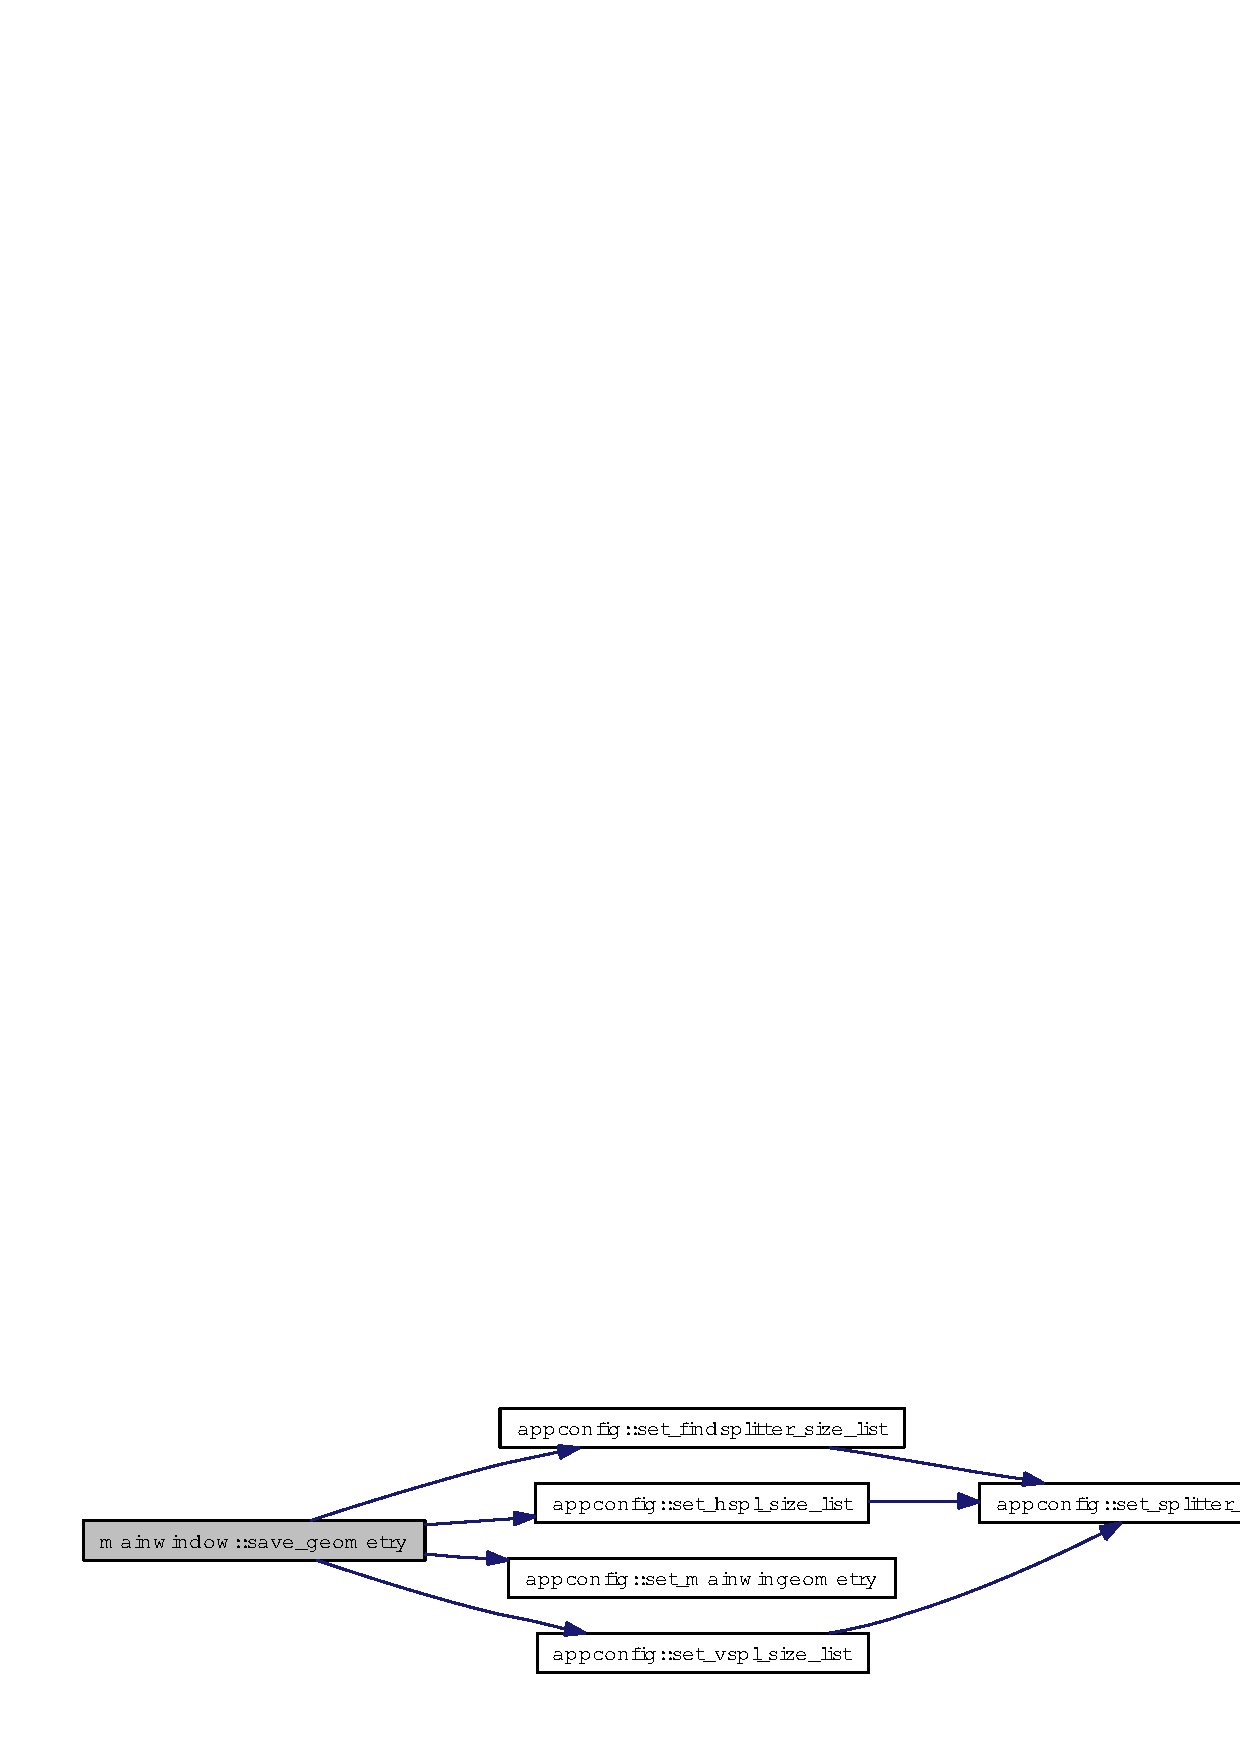
\includegraphics[width=324pt]{classmainwindow_129c1ed40a92e5bbc43a7af90575ab6c_cgraph}
\end{center}
\end{figure}


Here is the caller graph for this function:\begin{figure}[H]
\begin{center}
\leavevmode
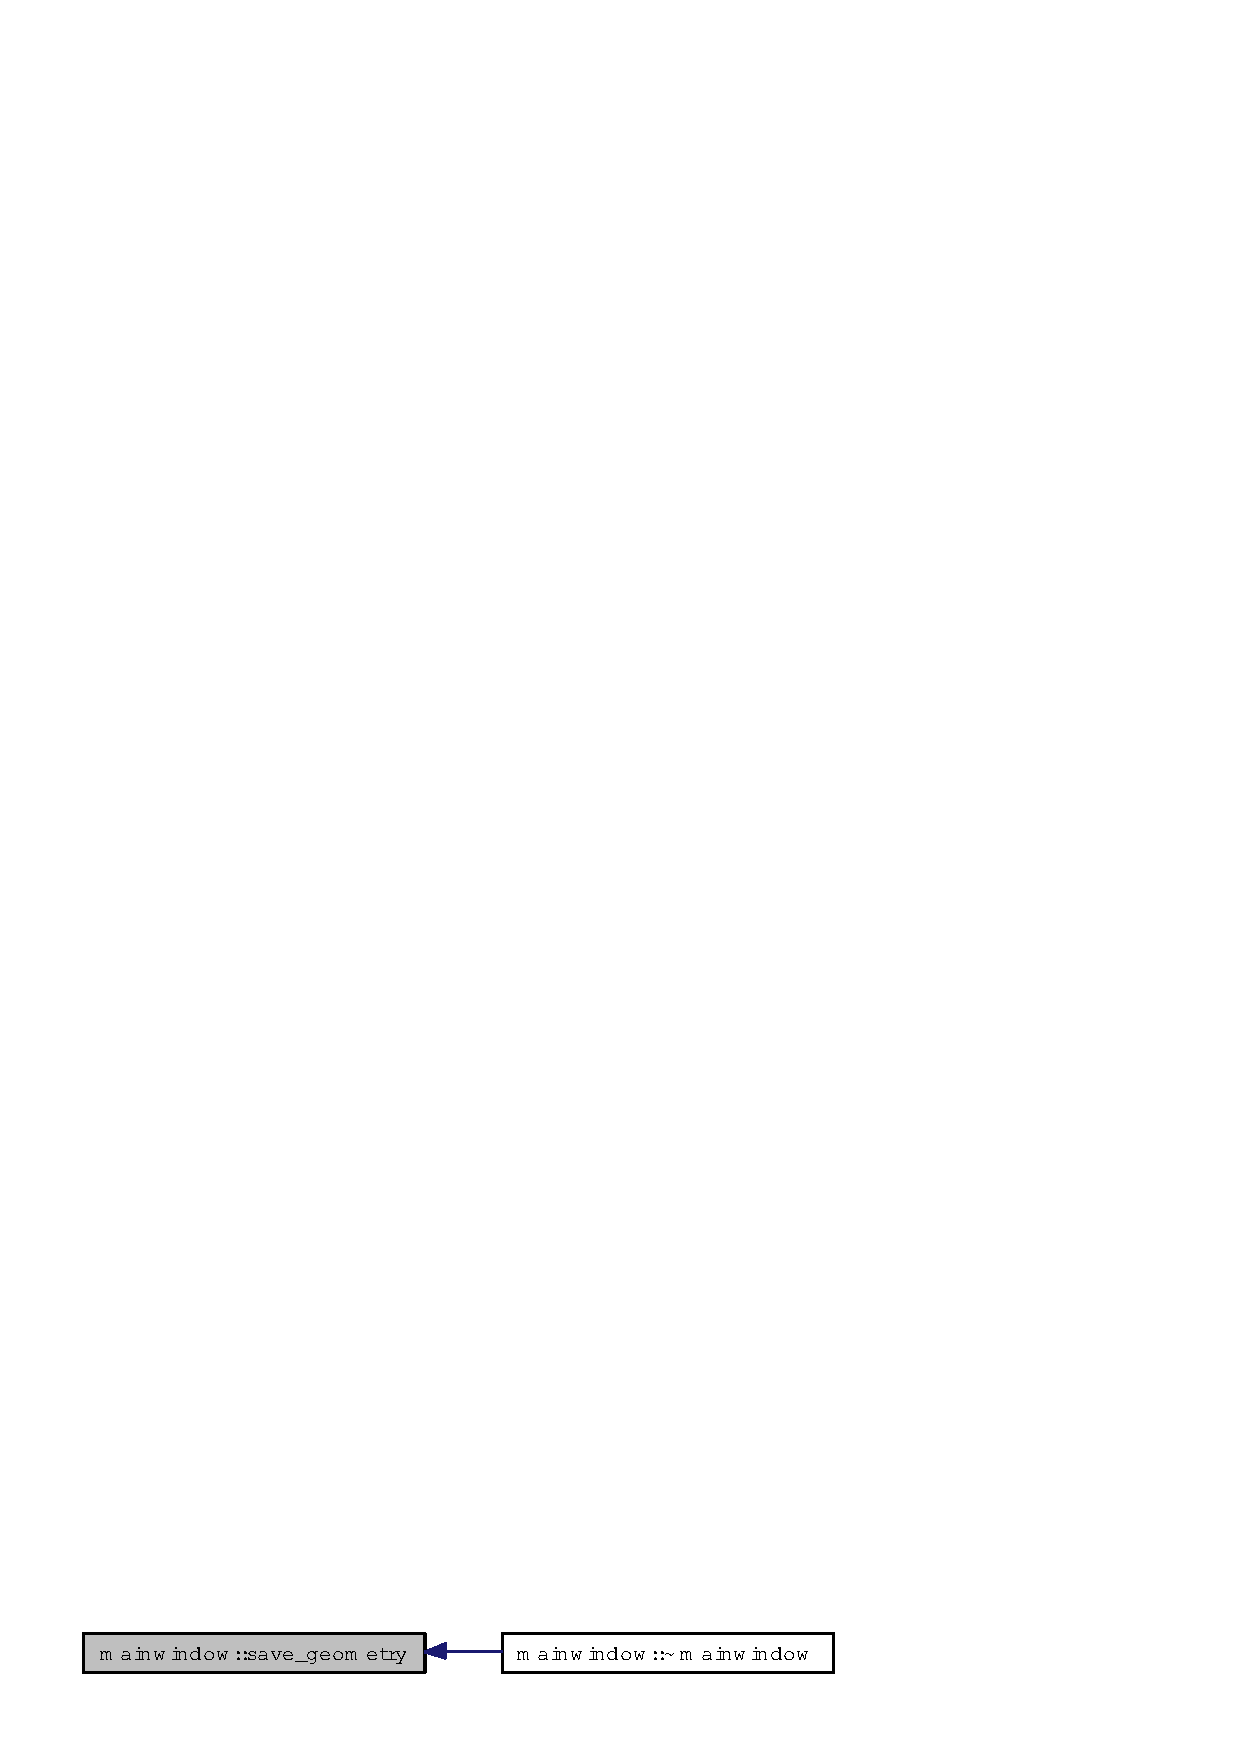
\includegraphics[width=202pt]{classmainwindow_129c1ed40a92e5bbc43a7af90575ab6c_icgraph}
\end{center}
\end{figure}
\index{mainwindow@{mainwindow}!save_tree_position@{save\_\-tree\_\-position}}
\index{save_tree_position@{save\_\-tree\_\-position}!mainwindow@{mainwindow}}
\subsubsection{\setlength{\rightskip}{0pt plus 5cm}void mainwindow::save\_\-tree\_\-position (void)\hspace{0.3cm}{\tt  [private]}}\label{classmainwindow_aa0957056623adcd87ea0d28c2e9f671}




Definition at line 133 of file mainwindow.cpp.

References treescreen::get\_\-current\_\-item\_\-index(), Tree\-Item::get\_\-path(), Tree\-Model::get\-Item(), treescreen::kntrmodel, mytetraconfig, appconfig::set\_\-tree\_\-position(), and treeview.

Referenced by $\sim$mainwindow().

Here is the call graph for this function:\begin{figure}[H]
\begin{center}
\leavevmode
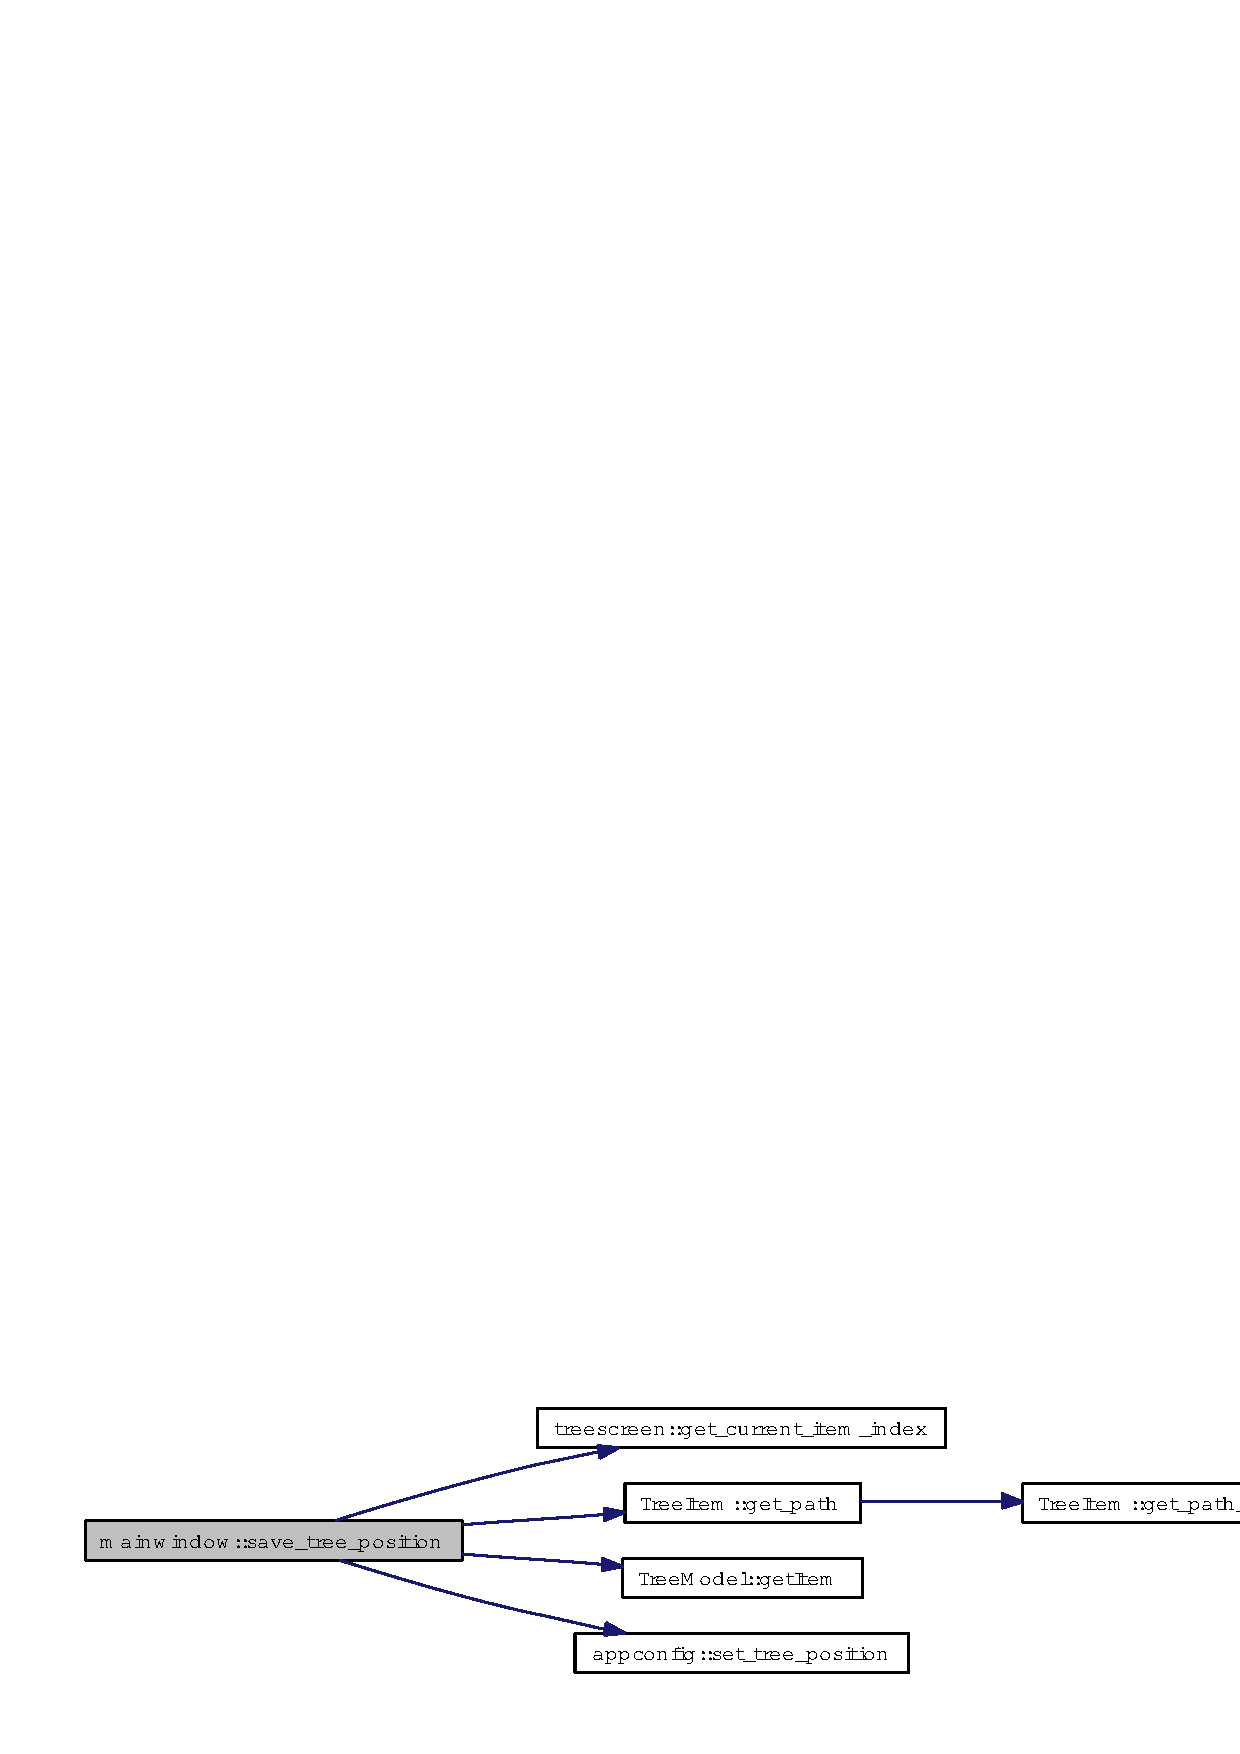
\includegraphics[width=395pt]{classmainwindow_aa0957056623adcd87ea0d28c2e9f671_cgraph}
\end{center}
\end{figure}


Here is the caller graph for this function:\begin{figure}[H]
\begin{center}
\leavevmode
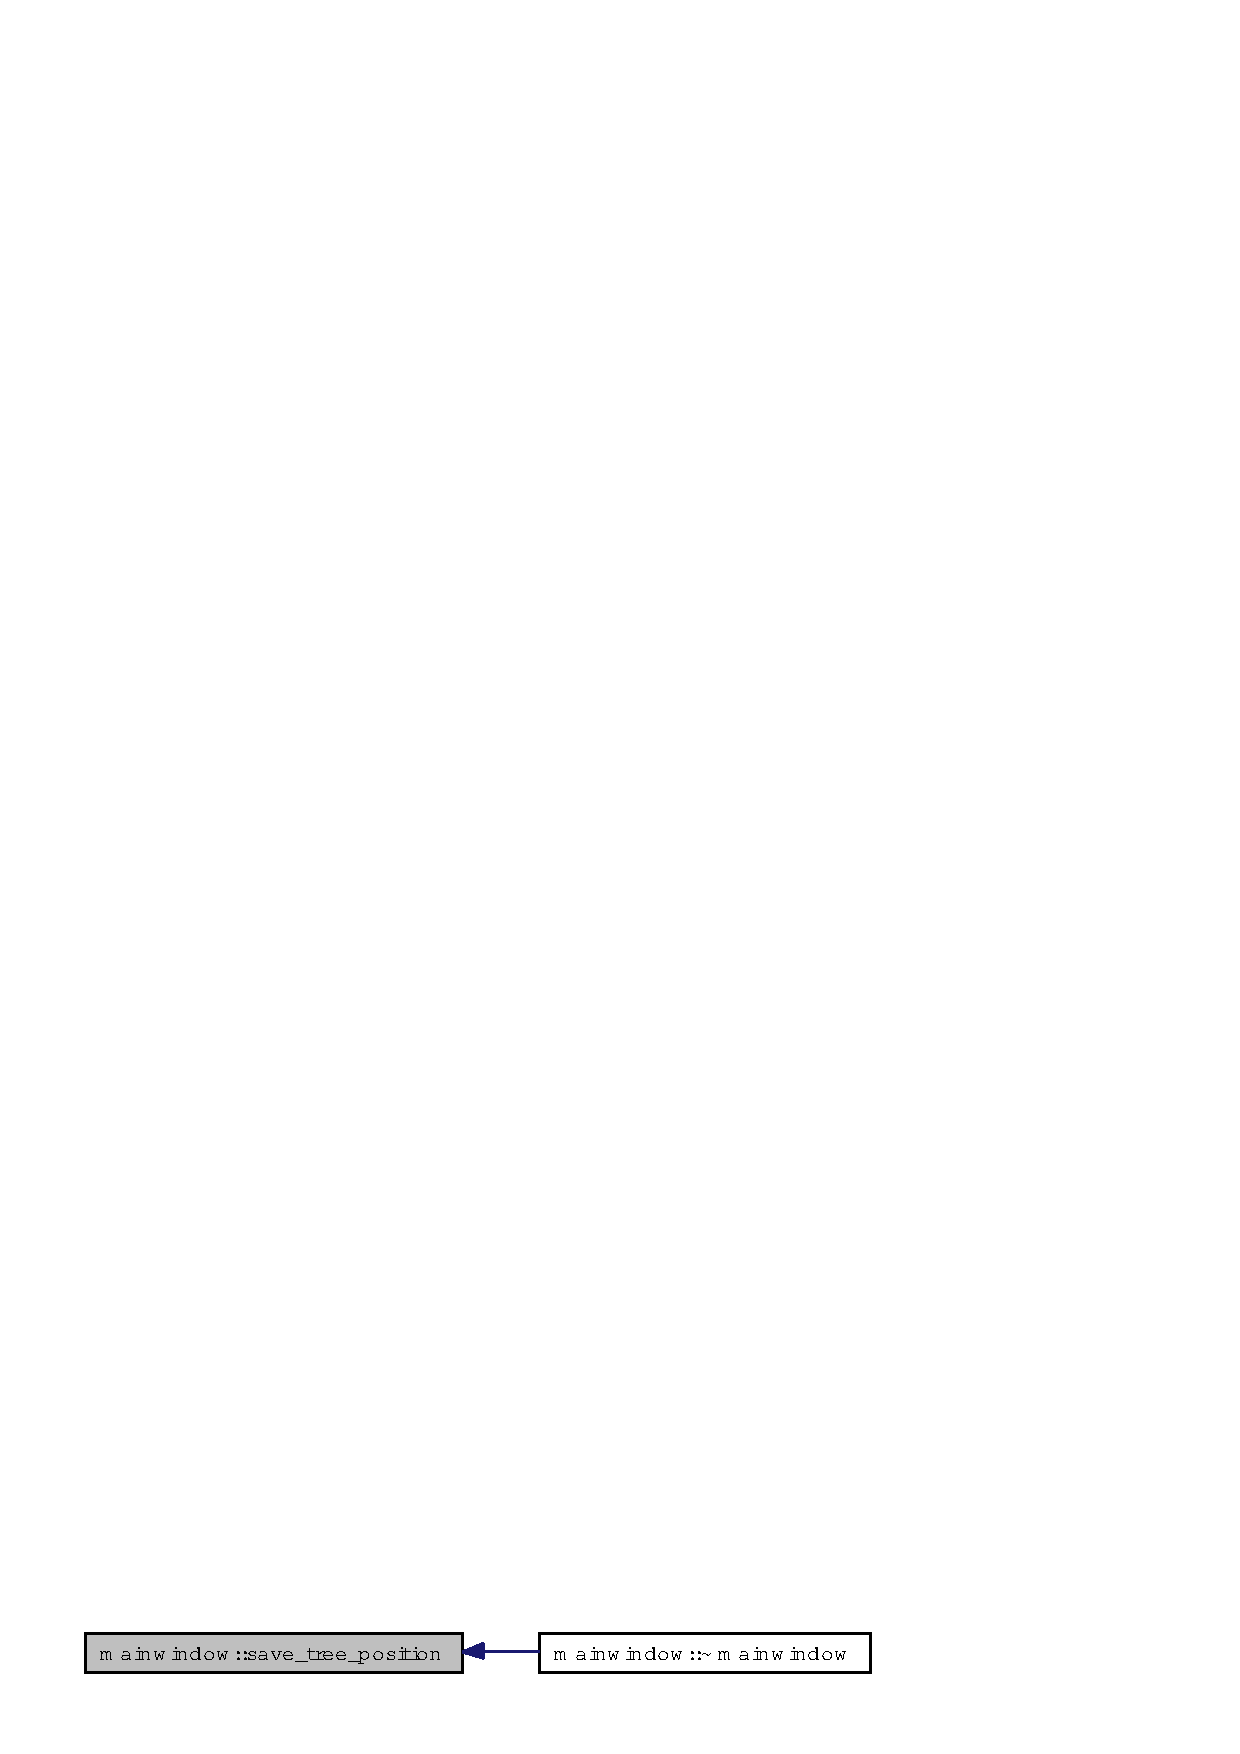
\includegraphics[width=211pt]{classmainwindow_aa0957056623adcd87ea0d28c2e9f671_icgraph}
\end{center}
\end{figure}
\index{mainwindow@{mainwindow}!save_recordtable_position@{save\_\-recordtable\_\-position}}
\index{save_recordtable_position@{save\_\-recordtable\_\-position}!mainwindow@{mainwindow}}
\subsubsection{\setlength{\rightskip}{0pt plus 5cm}void mainwindow::save\_\-recordtable\_\-position (void)\hspace{0.3cm}{\tt  [private]}}\label{classmainwindow_de588e1f1c0cc027d50038e075c90de2}




Definition at line 169 of file mainwindow.cpp.

References recordtablescreen::get\_\-first\_\-selection\_\-pos(), mytetraconfig, recordtableview, and appconfig::set\_\-recordtable\_\-position().

Referenced by $\sim$mainwindow().

Here is the call graph for this function:\begin{figure}[H]
\begin{center}
\leavevmode
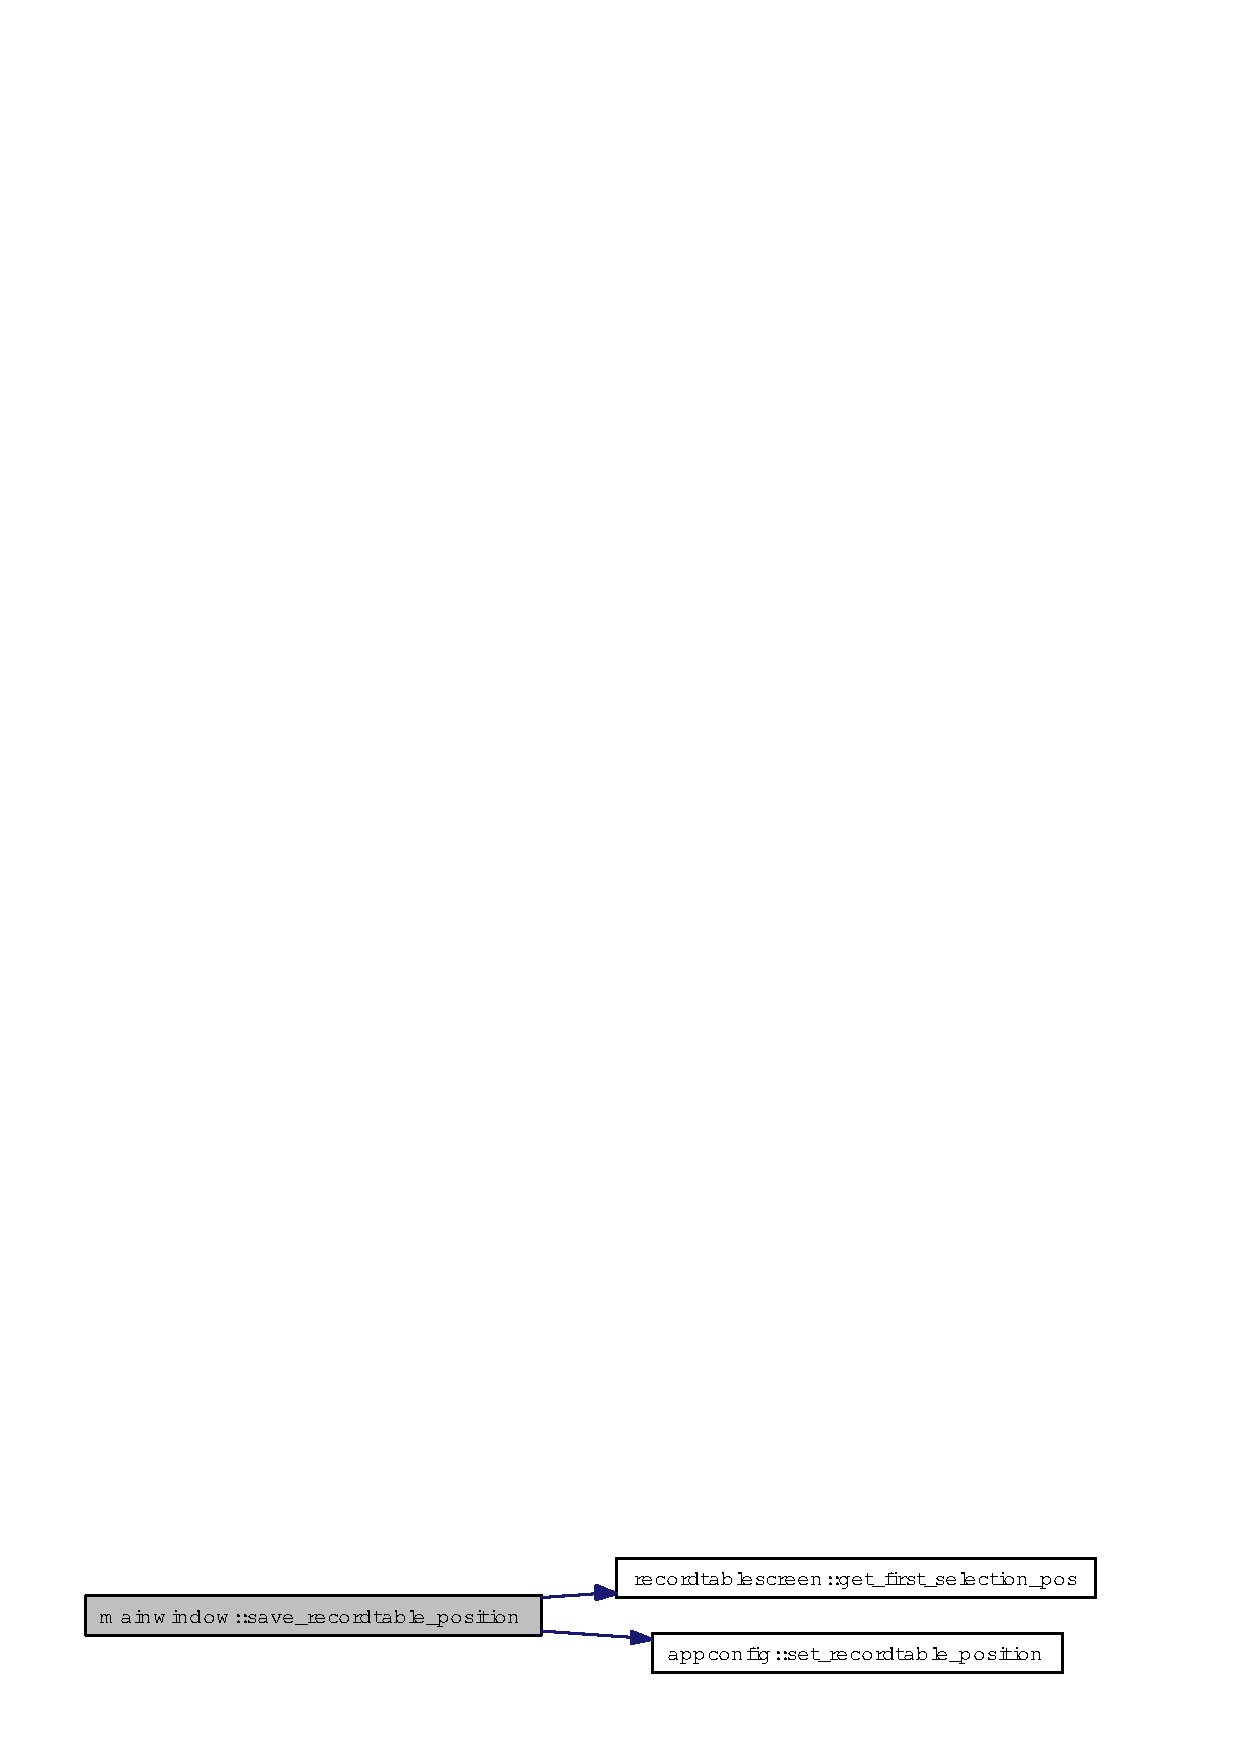
\includegraphics[width=265pt]{classmainwindow_de588e1f1c0cc027d50038e075c90de2_cgraph}
\end{center}
\end{figure}


Here is the caller graph for this function:\begin{figure}[H]
\begin{center}
\leavevmode
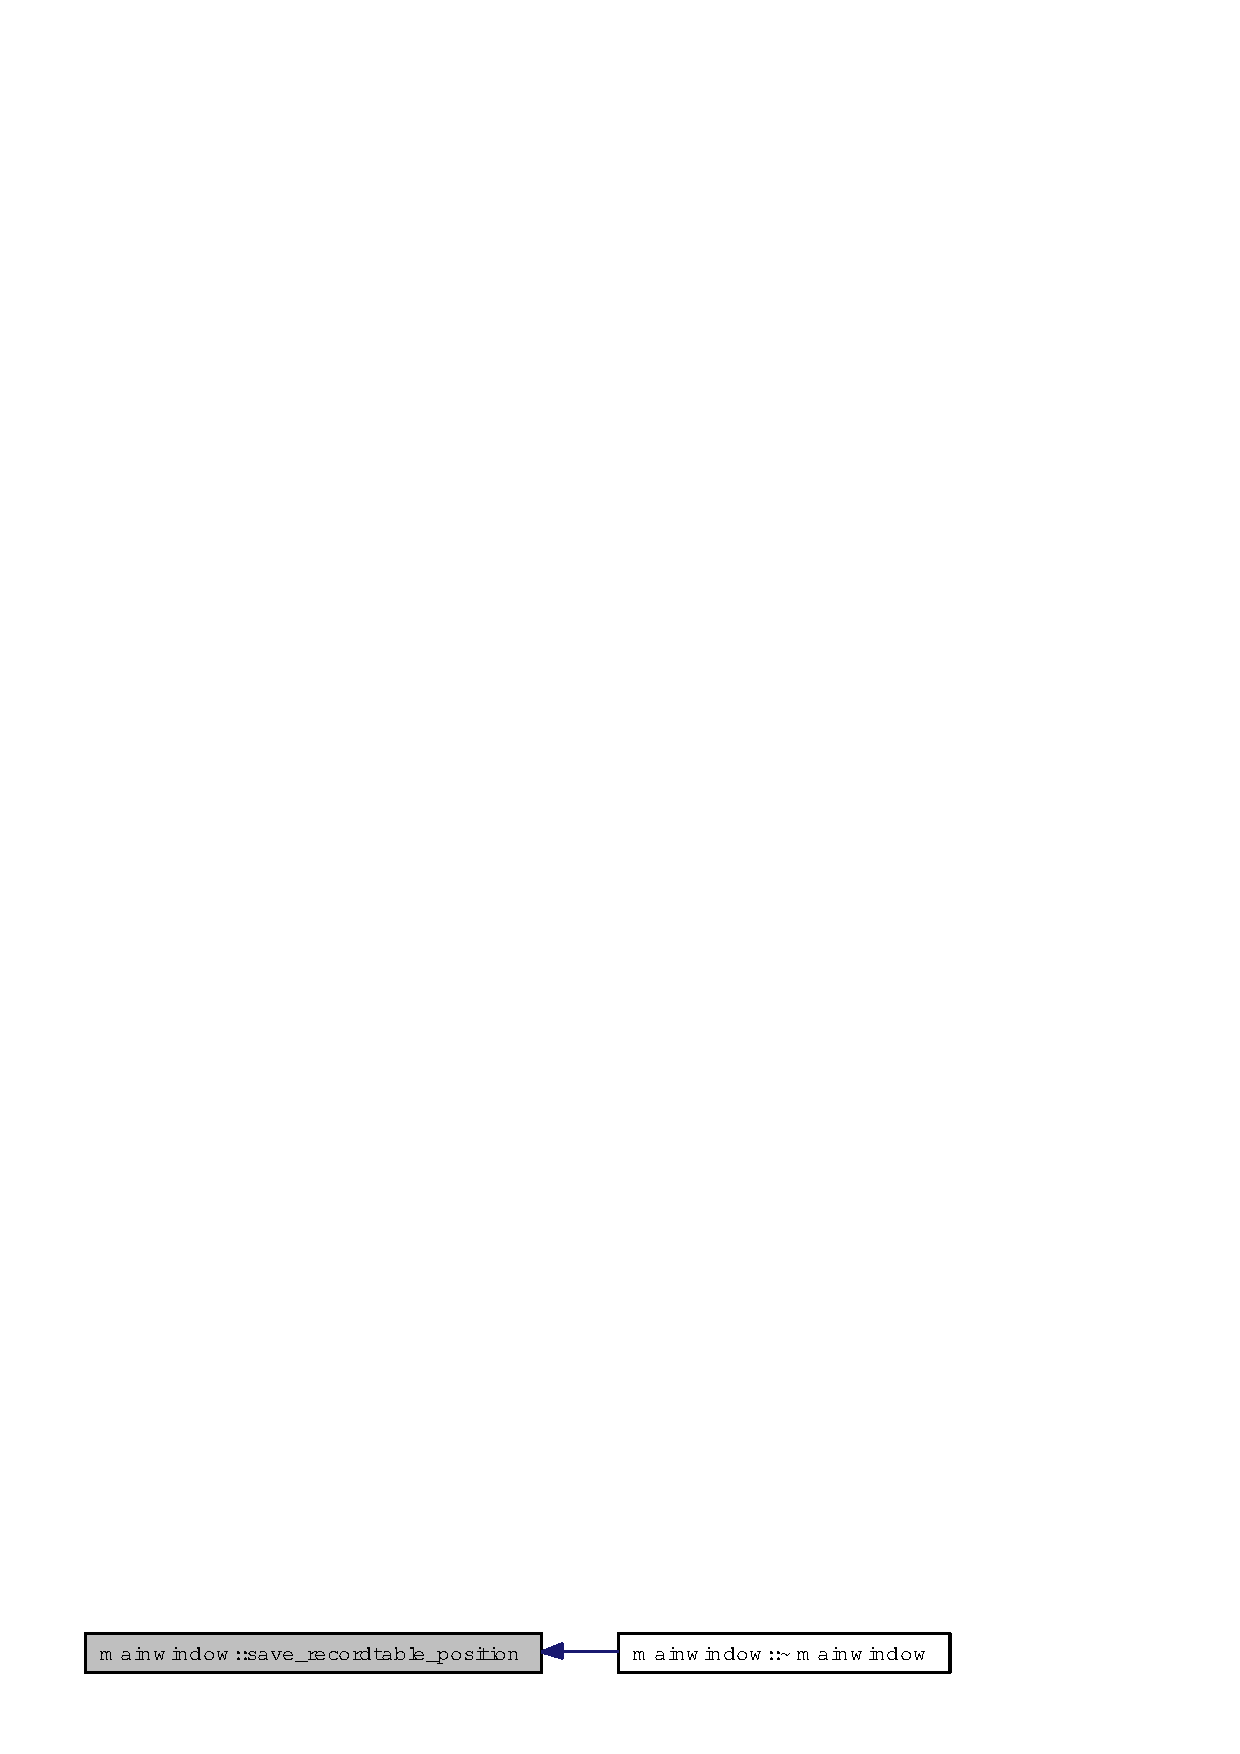
\includegraphics[width=230pt]{classmainwindow_de588e1f1c0cc027d50038e075c90de2_icgraph}
\end{center}
\end{figure}
\index{mainwindow@{mainwindow}!closeEvent@{closeEvent}}
\index{closeEvent@{closeEvent}!mainwindow@{mainwindow}}
\subsubsection{\setlength{\rightskip}{0pt plus 5cm}void mainwindow::close\-Event (QClose\-Event $\ast$ {\em event})\hspace{0.3cm}{\tt  [protected]}}\label{classmainwindow_538c6f8c44d0545ac6124c43ce261e87}




Definition at line 401 of file mainwindow.cpp.

References tray\_\-icon.

\subsection{Member Data Documentation}
\index{mainwindow@{mainwindow}!treeview@{treeview}}
\index{treeview@{treeview}!mainwindow@{mainwindow}}
\subsubsection{\setlength{\rightskip}{0pt plus 5cm}{\bf treescreen}$\ast$ {\bf mainwindow::treeview}}\label{classmainwindow_edd9c2c38ab9071fc3f7a3817fb3b84f}




Definition at line 79 of file mainwindow.h.

Referenced by assembly(), save\_\-tree\_\-position(), set\_\-tree\_\-position(), setup\_\-ui(), and $\sim$mainwindow().\index{mainwindow@{mainwindow}!recordtableview@{recordtableview}}
\index{recordtableview@{recordtableview}!mainwindow@{mainwindow}}
\subsubsection{\setlength{\rightskip}{0pt plus 5cm}{\bf recordtablescreen}$\ast$ {\bf mainwindow::recordtableview}}\label{classmainwindow_e52eec38c847f7b2bac07ef4bd2a589b}




Definition at line 80 of file mainwindow.h.

Referenced by assembly(), save\_\-current\_\-record\_\-text(), save\_\-recordtable\_\-position(), set\_\-recordtable\_\-position(), setup\_\-ui(), and $\sim$mainwindow().\index{mainwindow@{mainwindow}!editorview@{editorview}}
\index{editorview@{editorview}!mainwindow@{mainwindow}}
\subsubsection{\setlength{\rightskip}{0pt plus 5cm}{\bf metaeditor}$\ast$ {\bf mainwindow::editorview}}\label{classmainwindow_96cc8a1a6f9aee956a2fc66edc6977e1}




Definition at line 81 of file mainwindow.h.

Referenced by assembly(), file\-Print(), file\-Print\-Pdf(), file\-Print\-Preview(), save\_\-current\_\-record\_\-text(), setup\_\-ui(), and $\sim$mainwindow().\index{mainwindow@{mainwindow}!findscreendisp@{findscreendisp}}
\index{findscreendisp@{findscreendisp}!mainwindow@{mainwindow}}
\subsubsection{\setlength{\rightskip}{0pt plus 5cm}{\bf findscreen}$\ast$ {\bf mainwindow::findscreendisp}}\label{classmainwindow_d5588e5a249f88dba16dec4906017fc0}




Definition at line 82 of file mainwindow.h.

Referenced by assembly(), save\_\-geometry(), and setup\_\-ui().\index{mainwindow@{mainwindow}!statbar@{statbar}}
\index{statbar@{statbar}!mainwindow@{mainwindow}}
\subsubsection{\setlength{\rightskip}{0pt plus 5cm}QStatus\-Bar$\ast$ {\bf mainwindow::statbar}}\label{classmainwindow_c60f859bf7c9f4eafc2e2da3e88f1fb4}




Definition at line 83 of file mainwindow.h.

Referenced by setup\_\-ui().\index{mainwindow@{mainwindow}!tray_restore_action@{tray\_\-restore\_\-action}}
\index{tray_restore_action@{tray\_\-restore\_\-action}!mainwindow@{mainwindow}}
\subsubsection{\setlength{\rightskip}{0pt plus 5cm}QAction$\ast$ {\bf mainwindow::tray\_\-restore\_\-action}\hspace{0.3cm}{\tt  [private]}}\label{classmainwindow_c3fe87e5828b746da19f9c9f952155c5}




Definition at line 125 of file mainwindow.h.

Referenced by create\_\-tray\_\-icon(), and setup\_\-icon\_\-actions().\index{mainwindow@{mainwindow}!tray_maximize_action@{tray\_\-maximize\_\-action}}
\index{tray_maximize_action@{tray\_\-maximize\_\-action}!mainwindow@{mainwindow}}
\subsubsection{\setlength{\rightskip}{0pt plus 5cm}QAction$\ast$ {\bf mainwindow::tray\_\-maximize\_\-action}\hspace{0.3cm}{\tt  [private]}}\label{classmainwindow_a694d5989b9fecd7bf3ebb325d700b3e}




Definition at line 126 of file mainwindow.h.

Referenced by create\_\-tray\_\-icon(), and setup\_\-icon\_\-actions().\index{mainwindow@{mainwindow}!tray_minimize_action@{tray\_\-minimize\_\-action}}
\index{tray_minimize_action@{tray\_\-minimize\_\-action}!mainwindow@{mainwindow}}
\subsubsection{\setlength{\rightskip}{0pt plus 5cm}QAction$\ast$ {\bf mainwindow::tray\_\-minimize\_\-action}\hspace{0.3cm}{\tt  [private]}}\label{classmainwindow_5acb527a6ec5a0b23515dc9b79c7139b}




Definition at line 127 of file mainwindow.h.

Referenced by create\_\-tray\_\-icon(), and setup\_\-icon\_\-actions().\index{mainwindow@{mainwindow}!tray_quit_action@{tray\_\-quit\_\-action}}
\index{tray_quit_action@{tray\_\-quit\_\-action}!mainwindow@{mainwindow}}
\subsubsection{\setlength{\rightskip}{0pt plus 5cm}QAction$\ast$ {\bf mainwindow::tray\_\-quit\_\-action}\hspace{0.3cm}{\tt  [private]}}\label{classmainwindow_cde21d47407a20a9e298e0541988768d}




Definition at line 128 of file mainwindow.h.

Referenced by create\_\-tray\_\-icon(), and setup\_\-icon\_\-actions().\index{mainwindow@{mainwindow}!tray_icon@{tray\_\-icon}}
\index{tray_icon@{tray\_\-icon}!mainwindow@{mainwindow}}
\subsubsection{\setlength{\rightskip}{0pt plus 5cm}QSystem\-Tray\-Icon$\ast$ {\bf mainwindow::tray\_\-icon}\hspace{0.3cm}{\tt  [private]}}\label{classmainwindow_a50f5901ab52e087f4704784d49d25d7}




Definition at line 130 of file mainwindow.h.

Referenced by close\-Event(), create\_\-tray\_\-icon(), mainwindow(), and set\_\-icon().\index{mainwindow@{mainwindow}!tray_icon_menu@{tray\_\-icon\_\-menu}}
\index{tray_icon_menu@{tray\_\-icon\_\-menu}!mainwindow@{mainwindow}}
\subsubsection{\setlength{\rightskip}{0pt plus 5cm}QMenu$\ast$ {\bf mainwindow::tray\_\-icon\_\-menu}\hspace{0.3cm}{\tt  [private]}}\label{classmainwindow_f09dacf775049881fdd5c9f6ac429825}




Definition at line 131 of file mainwindow.h.

Referenced by create\_\-tray\_\-icon().\index{mainwindow@{mainwindow}!vspl@{vspl}}
\index{vspl@{vspl}!mainwindow@{mainwindow}}
\subsubsection{\setlength{\rightskip}{0pt plus 5cm}QSplitter$\ast$ {\bf mainwindow::vspl}\hspace{0.3cm}{\tt  [private]}}\label{classmainwindow_ed628404d778a22ab7faffa6328c9b7c}




Definition at line 133 of file mainwindow.h.

Referenced by assembly(), restore\_\-geometry(), and save\_\-geometry().\index{mainwindow@{mainwindow}!hspl@{hspl}}
\index{hspl@{hspl}!mainwindow@{mainwindow}}
\subsubsection{\setlength{\rightskip}{0pt plus 5cm}QSplitter$\ast$ {\bf mainwindow::hspl}\hspace{0.3cm}{\tt  [private]}}\label{classmainwindow_8b5d623b46b8e181a5152b503d055b54}




Definition at line 134 of file mainwindow.h.

Referenced by assembly(), restore\_\-geometry(), and save\_\-geometry().\index{mainwindow@{mainwindow}!findsplitter@{findsplitter}}
\index{findsplitter@{findsplitter}!mainwindow@{mainwindow}}
\subsubsection{\setlength{\rightskip}{0pt plus 5cm}QSplitter$\ast$ {\bf mainwindow::findsplitter}\hspace{0.3cm}{\tt  [private]}}\label{classmainwindow_432d81c9fadef4dd528d86c0e9135600}




Definition at line 135 of file mainwindow.h.

Referenced by assembly(), restore\_\-geometry(), and save\_\-geometry().

The documentation for this class was generated from the following files:\begin{CompactItemize}
\item 
{\bf mainwindow.h}\item 
{\bf mainwindow.cpp}\end{CompactItemize}
